\documentclass[12pt,a4paper,twoside,openright]{book}

\usepackage[utf8]{inputenc}
\usepackage[italian]{babel}
\usepackage[T1]{fontenc}

\usepackage{style/isi_style_lt}

\usepackage{amsmath,amsfonts,amssymb,amsthm}
\usepackage{caption}
\usepackage[usenames]{color}
\usepackage{enumerate}
\usepackage{fancyhdr}
\usepackage{fancyvrb}
\usepackage{float}
\usepackage{graphicx}
\usepackage{booktabs}
\usepackage{indentfirst}
\usepackage{listings}
\usepackage{marvosym}
\usepackage{multicol}
\usepackage{sectsty}
\usepackage{subcaption}
\usepackage{tocloft}
\usepackage{microtype}
\usepackage[table]{xcolor}
\usepackage{url}
\usepackage{hyperref}
\usepackage{adjustbox}
\usepackage{tikz}
\usetikzlibrary{positioning, arrows.meta, shapes.geometric, shadows, shapes, arrows}
\usepackage{pgf-umlsd}
\usepackage{booktabs}
\usepackage{style/python}





    \usepackage{adjustbox} % Used to constrain images to a maximum size 
    \usepackage{textcomp} % defines textquotesingle
    % Hack from http://tex.stackexchange.com/a/47451/13684:
    \AtBeginDocument{%
        \def\PYZsq{\textquotesingle}% Upright quotes in Pygmentized code
    }
    \usepackage{upquote} % Upright quotes for verbatim code
    \usepackage{eurosym} % defines \euro
    \usepackage[mathletters]{ucs} % Extended unicode (utf-8) support
    \usepackage{grffile} % extends the file name processing of package graphics 
                         % to support a larger range 
    \usepackage{longtable} % longtable support required by pandoc >1.10
    \usepackage{booktabs}  % table support for pandoc > 1.12.2
    \usepackage[inline]{enumitem} % IRkernel/repr support (it uses the enumerate* environment)
    \usepackage[normalem]{ulem} % ulem is needed to support strikethroughs (\sout)

    
    % Colors for the hyperref package
    \definecolor{urlcolor}{rgb}{0,.145,.698}
    \definecolor{linkcolor}{rgb}{.71,0.21,0.01}
    \definecolor{citecolor}{rgb}{.12,.54,.11}

    % ANSI colors
    \definecolor{ansi-black}{HTML}{3E424D}
    \definecolor{ansi-black-intense}{HTML}{282C36}
    \definecolor{ansi-red}{HTML}{E75C58}
    \definecolor{ansi-red-intense}{HTML}{B22B31}
    \definecolor{ansi-green}{HTML}{00A250}
    \definecolor{ansi-green-intense}{HTML}{007427}
    \definecolor{ansi-yellow}{HTML}{DDB62B}
    \definecolor{ansi-yellow-intense}{HTML}{B27D12}
    \definecolor{ansi-blue}{HTML}{208FFB}
    \definecolor{ansi-blue-intense}{HTML}{0065CA}
    \definecolor{ansi-magenta}{HTML}{D160C4}
    \definecolor{ansi-magenta-intense}{HTML}{A03196}
    \definecolor{ansi-cyan}{HTML}{60C6C8}
    \definecolor{ansi-cyan-intense}{HTML}{258F8F}
    \definecolor{ansi-white}{HTML}{C5C1B4}
    \definecolor{ansi-white-intense}{HTML}{A1A6B2}

    % commands and environments needed by pandoc snippets
    % extracted from the output of `pandoc -s`
    \providecommand{\tightlist}{%
      \setlength{\itemsep}{0pt}\setlength{\parskip}{0pt}}
    \DefineVerbatimEnvironment{Highlighting}{Verbatim}{commandchars=\\\{\}}
    % Add ',fontsize=\small' for more characters per line
    \newenvironment{Shaded}{}{}
    \newcommand{\KeywordTok}[1]{\textcolor[rgb]{0.00,0.44,0.13}{\textbf{{#1}}}}
    \newcommand{\DataTypeTok}[1]{\textcolor[rgb]{0.56,0.13,0.00}{{#1}}}
    \newcommand{\DecValTok}[1]{\textcolor[rgb]{0.25,0.63,0.44}{{#1}}}
    \newcommand{\BaseNTok}[1]{\textcolor[rgb]{0.25,0.63,0.44}{{#1}}}
    \newcommand{\FloatTok}[1]{\textcolor[rgb]{0.25,0.63,0.44}{{#1}}}
    \newcommand{\CharTok}[1]{\textcolor[rgb]{0.25,0.44,0.63}{{#1}}}
    \newcommand{\StringTok}[1]{\textcolor[rgb]{0.25,0.44,0.63}{{#1}}}
    \newcommand{\CommentTok}[1]{\textcolor[rgb]{0.38,0.63,0.69}{\textit{{#1}}}}
    \newcommand{\OtherTok}[1]{\textcolor[rgb]{0.00,0.44,0.13}{{#1}}}
    \newcommand{\AlertTok}[1]{\textcolor[rgb]{1.00,0.00,0.00}{\textbf{{#1}}}}
    \newcommand{\FunctionTok}[1]{\textcolor[rgb]{0.02,0.16,0.49}{{#1}}}
    \newcommand{\RegionMarkerTok}[1]{{#1}}
    \newcommand{\ErrorTok}[1]{\textcolor[rgb]{1.00,0.00,0.00}{\textbf{{#1}}}}
    \newcommand{\NormalTok}[1]{{#1}}
    
    % Additional commands for more recent versions of Pandoc
    \newcommand{\ConstantTok}[1]{\textcolor[rgb]{0.53,0.00,0.00}{{#1}}}
    \newcommand{\SpecialCharTok}[1]{\textcolor[rgb]{0.25,0.44,0.63}{{#1}}}
    \newcommand{\VerbatimStringTok}[1]{\textcolor[rgb]{0.25,0.44,0.63}{{#1}}}
    \newcommand{\SpecialStringTok}[1]{\textcolor[rgb]{0.73,0.40,0.53}{{#1}}}
    \newcommand{\ImportTok}[1]{{#1}}
    \newcommand{\DocumentationTok}[1]{\textcolor[rgb]{0.73,0.13,0.13}{\textit{{#1}}}}
    \newcommand{\AnnotationTok}[1]{\textcolor[rgb]{0.38,0.63,0.69}{\textbf{\textit{{#1}}}}}
    \newcommand{\CommentVarTok}[1]{\textcolor[rgb]{0.38,0.63,0.69}{\textbf{\textit{{#1}}}}}
    \newcommand{\VariableTok}[1]{\textcolor[rgb]{0.10,0.09,0.49}{{#1}}}
    \newcommand{\ControlFlowTok}[1]{\textcolor[rgb]{0.00,0.44,0.13}{\textbf{{#1}}}}
    \newcommand{\OperatorTok}[1]{\textcolor[rgb]{0.40,0.40,0.40}{{#1}}}
    \newcommand{\BuiltInTok}[1]{{#1}}
    \newcommand{\ExtensionTok}[1]{{#1}}
    \newcommand{\PreprocessorTok}[1]{\textcolor[rgb]{0.74,0.48,0.00}{{#1}}}
    \newcommand{\AttributeTok}[1]{\textcolor[rgb]{0.49,0.56,0.16}{{#1}}}
    \newcommand{\InformationTok}[1]{\textcolor[rgb]{0.38,0.63,0.69}{\textbf{\textit{{#1}}}}}
    \newcommand{\WarningTok}[1]{\textcolor[rgb]{0.38,0.63,0.69}{\textbf{\textit{{#1}}}}}
    
    
    % Define a nice break command that doesn't care if a line doesn't already
    % exist.
    \def\br{\hspace*{\fill} \\* }
    % Math Jax compatability definitions
    \def\gt{>}
    \def\lt{<}
    % Document parameters
    \title{Untitled1}
    
    
    

    % Pygments definitions
    
\makeatletter
\def\PY@reset{\let\PY@it=\relax \let\PY@bf=\relax%
    \let\PY@ul=\relax \let\PY@tc=\relax%
    \let\PY@bc=\relax \let\PY@ff=\relax}
\def\PY@tok#1{\csname PY@tok@#1\endcsname}
\def\PY@toks#1+{\ifx\relax#1\empty\else%
    \PY@tok{#1}\expandafter\PY@toks\fi}
\def\PY@do#1{\PY@bc{\PY@tc{\PY@ul{%
    \PY@it{\PY@bf{\PY@ff{#1}}}}}}}
\def\PY#1#2{\PY@reset\PY@toks#1+\relax+\PY@do{#2}}

\expandafter\def\csname PY@tok@w\endcsname{\def\PY@tc##1{\textcolor[rgb]{0.73,0.73,0.73}{##1}}}
\expandafter\def\csname PY@tok@c\endcsname{\let\PY@it=\textit\def\PY@tc##1{\textcolor[rgb]{0.25,0.50,0.50}{##1}}}
\expandafter\def\csname PY@tok@cp\endcsname{\def\PY@tc##1{\textcolor[rgb]{0.74,0.48,0.00}{##1}}}
\expandafter\def\csname PY@tok@k\endcsname{\let\PY@bf=\textbf\def\PY@tc##1{\textcolor[rgb]{0.00,0.50,0.00}{##1}}}
\expandafter\def\csname PY@tok@kp\endcsname{\def\PY@tc##1{\textcolor[rgb]{0.00,0.50,0.00}{##1}}}
\expandafter\def\csname PY@tok@kt\endcsname{\def\PY@tc##1{\textcolor[rgb]{0.69,0.00,0.25}{##1}}}
\expandafter\def\csname PY@tok@o\endcsname{\def\PY@tc##1{\textcolor[rgb]{0.40,0.40,0.40}{##1}}}
\expandafter\def\csname PY@tok@ow\endcsname{\let\PY@bf=\textbf\def\PY@tc##1{\textcolor[rgb]{0.67,0.13,1.00}{##1}}}
\expandafter\def\csname PY@tok@nb\endcsname{\def\PY@tc##1{\textcolor[rgb]{0.00,0.50,0.00}{##1}}}
\expandafter\def\csname PY@tok@nf\endcsname{\def\PY@tc##1{\textcolor[rgb]{0.00,0.00,1.00}{##1}}}
\expandafter\def\csname PY@tok@nc\endcsname{\let\PY@bf=\textbf\def\PY@tc##1{\textcolor[rgb]{0.00,0.00,1.00}{##1}}}
\expandafter\def\csname PY@tok@nn\endcsname{\let\PY@bf=\textbf\def\PY@tc##1{\textcolor[rgb]{0.00,0.00,1.00}{##1}}}
\expandafter\def\csname PY@tok@ne\endcsname{\let\PY@bf=\textbf\def\PY@tc##1{\textcolor[rgb]{0.82,0.25,0.23}{##1}}}
\expandafter\def\csname PY@tok@nv\endcsname{\def\PY@tc##1{\textcolor[rgb]{0.10,0.09,0.49}{##1}}}
\expandafter\def\csname PY@tok@no\endcsname{\def\PY@tc##1{\textcolor[rgb]{0.53,0.00,0.00}{##1}}}
\expandafter\def\csname PY@tok@nl\endcsname{\def\PY@tc##1{\textcolor[rgb]{0.63,0.63,0.00}{##1}}}
\expandafter\def\csname PY@tok@ni\endcsname{\let\PY@bf=\textbf\def\PY@tc##1{\textcolor[rgb]{0.60,0.60,0.60}{##1}}}
\expandafter\def\csname PY@tok@na\endcsname{\def\PY@tc##1{\textcolor[rgb]{0.49,0.56,0.16}{##1}}}
\expandafter\def\csname PY@tok@nt\endcsname{\let\PY@bf=\textbf\def\PY@tc##1{\textcolor[rgb]{0.00,0.50,0.00}{##1}}}
\expandafter\def\csname PY@tok@nd\endcsname{\def\PY@tc##1{\textcolor[rgb]{0.67,0.13,1.00}{##1}}}
\expandafter\def\csname PY@tok@s\endcsname{\def\PY@tc##1{\textcolor[rgb]{0.73,0.13,0.13}{##1}}}
\expandafter\def\csname PY@tok@sd\endcsname{\let\PY@it=\textit\def\PY@tc##1{\textcolor[rgb]{0.73,0.13,0.13}{##1}}}
\expandafter\def\csname PY@tok@si\endcsname{\let\PY@bf=\textbf\def\PY@tc##1{\textcolor[rgb]{0.73,0.40,0.53}{##1}}}
\expandafter\def\csname PY@tok@se\endcsname{\let\PY@bf=\textbf\def\PY@tc##1{\textcolor[rgb]{0.73,0.40,0.13}{##1}}}
\expandafter\def\csname PY@tok@sr\endcsname{\def\PY@tc##1{\textcolor[rgb]{0.73,0.40,0.53}{##1}}}
\expandafter\def\csname PY@tok@ss\endcsname{\def\PY@tc##1{\textcolor[rgb]{0.10,0.09,0.49}{##1}}}
\expandafter\def\csname PY@tok@sx\endcsname{\def\PY@tc##1{\textcolor[rgb]{0.00,0.50,0.00}{##1}}}
\expandafter\def\csname PY@tok@m\endcsname{\def\PY@tc##1{\textcolor[rgb]{0.40,0.40,0.40}{##1}}}
\expandafter\def\csname PY@tok@gh\endcsname{\let\PY@bf=\textbf\def\PY@tc##1{\textcolor[rgb]{0.00,0.00,0.50}{##1}}}
\expandafter\def\csname PY@tok@gu\endcsname{\let\PY@bf=\textbf\def\PY@tc##1{\textcolor[rgb]{0.50,0.00,0.50}{##1}}}
\expandafter\def\csname PY@tok@gd\endcsname{\def\PY@tc##1{\textcolor[rgb]{0.63,0.00,0.00}{##1}}}
\expandafter\def\csname PY@tok@gi\endcsname{\def\PY@tc##1{\textcolor[rgb]{0.00,0.63,0.00}{##1}}}
\expandafter\def\csname PY@tok@gr\endcsname{\def\PY@tc##1{\textcolor[rgb]{1.00,0.00,0.00}{##1}}}
\expandafter\def\csname PY@tok@ge\endcsname{\let\PY@it=\textit}
\expandafter\def\csname PY@tok@gs\endcsname{\let\PY@bf=\textbf}
\expandafter\def\csname PY@tok@gp\endcsname{\let\PY@bf=\textbf\def\PY@tc##1{\textcolor[rgb]{0.00,0.00,0.50}{##1}}}
\expandafter\def\csname PY@tok@go\endcsname{\def\PY@tc##1{\textcolor[rgb]{0.53,0.53,0.53}{##1}}}
\expandafter\def\csname PY@tok@gt\endcsname{\def\PY@tc##1{\textcolor[rgb]{0.00,0.27,0.87}{##1}}}
\expandafter\def\csname PY@tok@err\endcsname{\def\PY@bc##1{\setlength{\fboxsep}{0pt}\fcolorbox[rgb]{1.00,0.00,0.00}{1,1,1}{\strut ##1}}}
\expandafter\def\csname PY@tok@kc\endcsname{\let\PY@bf=\textbf\def\PY@tc##1{\textcolor[rgb]{0.00,0.50,0.00}{##1}}}
\expandafter\def\csname PY@tok@kd\endcsname{\let\PY@bf=\textbf\def\PY@tc##1{\textcolor[rgb]{0.00,0.50,0.00}{##1}}}
\expandafter\def\csname PY@tok@kn\endcsname{\let\PY@bf=\textbf\def\PY@tc##1{\textcolor[rgb]{0.00,0.50,0.00}{##1}}}
\expandafter\def\csname PY@tok@kr\endcsname{\let\PY@bf=\textbf\def\PY@tc##1{\textcolor[rgb]{0.00,0.50,0.00}{##1}}}
\expandafter\def\csname PY@tok@bp\endcsname{\def\PY@tc##1{\textcolor[rgb]{0.00,0.50,0.00}{##1}}}
\expandafter\def\csname PY@tok@fm\endcsname{\def\PY@tc##1{\textcolor[rgb]{0.00,0.00,1.00}{##1}}}
\expandafter\def\csname PY@tok@vc\endcsname{\def\PY@tc##1{\textcolor[rgb]{0.10,0.09,0.49}{##1}}}
\expandafter\def\csname PY@tok@vg\endcsname{\def\PY@tc##1{\textcolor[rgb]{0.10,0.09,0.49}{##1}}}
\expandafter\def\csname PY@tok@vi\endcsname{\def\PY@tc##1{\textcolor[rgb]{0.10,0.09,0.49}{##1}}}
\expandafter\def\csname PY@tok@vm\endcsname{\def\PY@tc##1{\textcolor[rgb]{0.10,0.09,0.49}{##1}}}
\expandafter\def\csname PY@tok@sa\endcsname{\def\PY@tc##1{\textcolor[rgb]{0.73,0.13,0.13}{##1}}}
\expandafter\def\csname PY@tok@sb\endcsname{\def\PY@tc##1{\textcolor[rgb]{0.73,0.13,0.13}{##1}}}
\expandafter\def\csname PY@tok@sc\endcsname{\def\PY@tc##1{\textcolor[rgb]{0.73,0.13,0.13}{##1}}}
\expandafter\def\csname PY@tok@dl\endcsname{\def\PY@tc##1{\textcolor[rgb]{0.73,0.13,0.13}{##1}}}
\expandafter\def\csname PY@tok@s2\endcsname{\def\PY@tc##1{\textcolor[rgb]{0.73,0.13,0.13}{##1}}}
\expandafter\def\csname PY@tok@sh\endcsname{\def\PY@tc##1{\textcolor[rgb]{0.73,0.13,0.13}{##1}}}
\expandafter\def\csname PY@tok@s1\endcsname{\def\PY@tc##1{\textcolor[rgb]{0.73,0.13,0.13}{##1}}}
\expandafter\def\csname PY@tok@mb\endcsname{\def\PY@tc##1{\textcolor[rgb]{0.40,0.40,0.40}{##1}}}
\expandafter\def\csname PY@tok@mf\endcsname{\def\PY@tc##1{\textcolor[rgb]{0.40,0.40,0.40}{##1}}}
\expandafter\def\csname PY@tok@mh\endcsname{\def\PY@tc##1{\textcolor[rgb]{0.40,0.40,0.40}{##1}}}
\expandafter\def\csname PY@tok@mi\endcsname{\def\PY@tc##1{\textcolor[rgb]{0.40,0.40,0.40}{##1}}}
\expandafter\def\csname PY@tok@il\endcsname{\def\PY@tc##1{\textcolor[rgb]{0.40,0.40,0.40}{##1}}}
\expandafter\def\csname PY@tok@mo\endcsname{\def\PY@tc##1{\textcolor[rgb]{0.40,0.40,0.40}{##1}}}
\expandafter\def\csname PY@tok@ch\endcsname{\let\PY@it=\textit\def\PY@tc##1{\textcolor[rgb]{0.25,0.50,0.50}{##1}}}
\expandafter\def\csname PY@tok@cm\endcsname{\let\PY@it=\textit\def\PY@tc##1{\textcolor[rgb]{0.25,0.50,0.50}{##1}}}
\expandafter\def\csname PY@tok@cpf\endcsname{\let\PY@it=\textit\def\PY@tc##1{\textcolor[rgb]{0.25,0.50,0.50}{##1}}}
\expandafter\def\csname PY@tok@c1\endcsname{\let\PY@it=\textit\def\PY@tc##1{\textcolor[rgb]{0.25,0.50,0.50}{##1}}}
\expandafter\def\csname PY@tok@cs\endcsname{\let\PY@it=\textit\def\PY@tc##1{\textcolor[rgb]{0.25,0.50,0.50}{##1}}}

\def\PYZbs{\char`\\}
\def\PYZus{\char`\_}
\def\PYZob{\char`\{}
\def\PYZcb{\char`\}}
\def\PYZca{\char`\^}
\def\PYZam{\char`\&}
\def\PYZlt{\char`\<}
\def\PYZgt{\char`\>}
\def\PYZsh{\char`\#}
\def\PYZpc{\char`\%}
\def\PYZdl{\char`\$}
\def\PYZhy{\char`\-}
\def\PYZsq{\char`\'}
\def\PYZdq{\char`\"}
\def\PYZti{\char`\~}
% for compatibility with earlier versions
\def\PYZat{@}
\def\PYZlb{[}
\def\PYZrb{]}
\makeatother


    % Exact colors from NB
    \definecolor{incolor}{rgb}{0.0, 0.0, 0.5}
    \definecolor{outcolor}{rgb}{0.545, 0.0, 0.0}




\hypersetup{%
	pdfpagemode={UseOutlines},
	bookmarksopen,
	pdfstartview={FitH},
	colorlinks,
	linkcolor={black},
	citecolor={black},
	urlcolor={black}
}

\AtBeginDocument{%
	\renewcommand{\contentsname}{Indice}
	\renewcommand\tablename{Tabella}
	\renewcommand\figurename{Figura}
	\renewcommand{\lstlistingname}{Listato}
	\renewcommand{\refname}{Riferimenti}
}

\definecolor{dkgreen}{rgb}{0,0.6,0}
\definecolor{gray}{rgb}{0.5,0.5,0.5}
\definecolor{mauve}{rgb}{0.58,0,0.82}
\definecolor{bracecolor}{rgb}{1, 0.788, 0.133}
\definecolor{keywordcolor}{rgb}{0.773, 0.376, 0.408}
\definecolor{stringcolor}{rgb}{0.780, 0.537, 0.839}
\definecolor{punct}{rgb}{0.0, 0.0, 0.0}
\definecolor{darkblue}{rgb}{0.0,0.0,0.6}
\definecolor{lightblue}{rgb}{0.0,0.0,0.9}
\definecolor{cyan}{rgb}{0.0,0.6,0.6}
\definecolor{darkred}{rgb}{0.6,0.0,0.0}

\definecolor{framecolor}{gray}{0.4} % Define the color for the frame

\DeclareFloatingEnvironment[
    fileext=loc,
    listname={List of Codes},
    name=Listato,
]{customcode}

\DeclareTCBListing{mintedbox}{O{}m!O{}}{
  listing engine=minted,
  listing only,
  minted language=#2,
  minted style=default,
  minted options={
    gobble=0,
    breaklines=true,
    breakafter=,,
    fontsize=\scriptsize,
    linenos,  
    #1},
  boxsep=3pt,
  left=3pt,
  right=3pt,
  top=3pt,
  bottom=3pt,
  arc=0pt,
  leftrule=0pt,
  rightrule=0pt,
  bottomrule=0pt,
  toprule=0pt,
  colback=white,
  colframe=framecolor,
  coltext=black,
  boxrule=0.5pt,
  overlay={},
  #3
}



\makeatletter
\def\cleardoublepage{
	\clearpage\if@twoside \ifodd\c@page\else
	\hbox{}
	\thispagestyle{empty}
	\newpage
	\if@twocolumn\hbox{}\newpage\fi\fi\fi
}

\makeatother

\setlength{\textwidth}{14cm}
\setlength{\textheight}{21cm}
\setlength{\footskip}{3cm}

\setlength{\hoffset}{0pt}
\setlength{\voffset}{0pt}

\setlength{\oddsidemargin}{1cm}
\setlength{\evensidemargin}{1cm}

\universita{Alma Mater Studiorum -- Università di Bologna}

\campus{Campus di Cesena}

\scuola{Scuola di Scienze}

\corsodilaurea{Corso di Laurea in Ingegneria e Scienze Informatiche}

\titolo{SciLay: Un Nuovo Dataset per Long Document Abstractive Summarization Tecnica e Lay di Articoli Biomedici}

\materia{Programmazione Di Applicazioni Data Intensive}

\laureando{Mattia Panni}

\relatore[Prof.]{Gianluca Moro}
\correlatoreA[Dott.]{Paolo Italiani}
\correlatoreB[Dott.]{Luca Ragazzi}

\sessione{Terza} 

\annoaccademico{2022 -- 2023}

\parolechiave 
{Abstractive Summarization}
{Natural Language Processing}
{Deep Neural Networks}
{Seq2Seq Models}
{Transformers}



\dedica{\emph{Il problema non è l'ascesa delle macchine ``intelligenti'', \\
                ma l'instupidimento dell'umanità.}\cite{books/gigerenzer/intelligenza}}

\makeindex

\begin{document}

\frontmatter 

\maketitle

\chapter*{Abstract}
\markboth{Abstract}{Abstract}

Questa tesi esplora il prospero settore dell'intelligenza artificiale (AI) e dell'elaborazione del linguaggio naturale (NLP), con l'obiettivo di automatizzare la creazione di riassunti comprensibili per gli articoli scientifici. Sfruttando metodologie AI all'avanguardia, questo studio si propone di ridurre il divario tra i dettagli intricati racchiusi nelle pubblicazioni scientifiche e la loro comprensione da parte del grande pubblico.

La complessità e la profondità tecnica degli articoli accademici spesso costituiscono una barriera alla comprensione generalizzata. Mentre gli abstract tecnici si rivolgono bene agli esperti del settore, possono risultare criptici per i ``non addetti ai lavori''. Affrontando questo divario comunicativo, la tesi propone un sistema automatizzato in grado di elaborare 'riassunti per il grande pubblico' o 'riassunti in linguaggio semplice', migliorando così l'accessibilità delle intuizioni scientifiche.

\newpage

\tableofcontents

\newpage

\listoffigures

\mainmatter

\pagestyle{fancy} 
\fancyhead[LO]{\nouppercase{\rightmark}}
\fancyhead[RE]{\nouppercase{\leftmark}}
\fancyhead[LE,RO]{\thepage}
\fancyfoot{}


%% CAPITOLO 1
\chapter{Introduzione}\label{cap:intro}

Di seguito, si delineano le basi concettuali e le motivazioni che hanno ispirato questa tesi, fornendo al lettore una panoramica del percorso di ricerca e delle innovazioni tecnologiche nell'ambito dell'intelligenza artificiale e del natural language processing, che hanno reso possibile l'ambizioso obiettivo di automatizzare la sintesi di riassunti accessibili di articoli scientifici.

\section{Intelligenza Artificiale}
L'\emph{intelligenza artificiale} (AI) è un campo interdisciplinare che si concentra sulla creazione di sistemi o macchine in grado di eseguire attività che richiedono, fra le altre cose

\begin{itemize}
    \item \textbf{Apprendimento automatico}. Le AI utilizzano tecniche di apprendimento automatico per acquisire conoscenze dai dati. Questo significa che anziché essere programmate esplicitamente per eseguire compiti specifici, come accade per gli algoritmi tradizionali, le AI apprendono dai dati e migliorano le loro prestazioni con l'esperienza. 
    \item \textbf{Generalizzazione}. Le AI sono in grado di adattarsi a nuove situazioni e compiti. Possono generalizzare le loro conoscenze per risolvere problemi simili a quelli affrontati durante l'addestramento. 
    \item \textbf{Processamento dei dati non strutturati}: Le AI sono spesso utilizzate per analizzare e comprendere dati non strutturati, come testo, immagini e suoni. Possono estrarre informazioni significative da fonti di dati complesse e rumorose.
\end{itemize}

Queste proprietà, auspicabili per tali sistemi, sono comunemente riconosciute come indicatori di intelligenza, da cui deriva il termine ``Intelligenza Artificiale''.

Questo campo è stato oggetto di ricerca e sviluppo fin dagli anni '50 ed è cresciuto enormemente in importanza e complessità. L'AI ha rivoluzionato molti aspetti della nostra vita, dai motori di ricerca online alla guida autonoma, dalla diagnosi medica all'automazione industriale. 

\subsection{Storia della nascita delle AI}
L'idea di creare macchine che possano simulare l'intelligenza umana ha radici antiche, ma il campo dell'AI moderna è iniziato nel 1956 con una conferenza tenuta a Dartmouth College, dove i ricercatori hanno discusso di ``programmare un computer per simulare l'intelligenza umana''. Questo evento è spesso considerato l'inizio ufficiale dell'AI come campo di studio.

Negli anni '50 e '60, gli studiosi dell'AI erano ottimisti riguardo alle potenzialità della disciplina. Credevano che sarebbe stato relativamente semplice programmare un computer per eseguire compiti che richiedevano intelligenza, come giocare a scacchi o tradurre lingue. Tuttavia, presto divenne chiaro che molte delle attività che gli esseri umani eseguono con facilità sono estremamente complesse da programmare.

Questo ha portato a un periodo noto come ``inverno dell'AI'' negli anni '70 e '80, durante il quale il finanziamento e l'interesse per l'AI diminuirono notevolmente. Ma negli anni '90, con l'aumento della potenza di calcolo, lo sviluppo di nuove tecniche e la disponibilità sempre maggiore di dati, l'AI ha conosciuto una rinascita. Oggi, l'AI è uno dei campi di ricerca e sviluppo più attivi al mondo.


\subsection{Limiti e Potenzialità delle AI}
D'altrocanto, come accade per ogni cosa, questo tipo di sistemi ottengono grandi risultati per un certo tipo di problemi, ma non per altri. Quando l'ambiente è stabile, ovvero presenta regole e/o pattern fissi (come nel caso degli scacchi), le AI eguagliano se non addirittura battono le performance degli esseri umani. Tuttavia, in situazioni colme di incertezza, potenza di calcolo elevata e disponibilità di grandi moli di dati contribuiscono in maniera limitata. In altre parole, al verificarsi di ``Cigni neri''\cite{books/taleb/cigno}, ovvero situazioni altamente improbabili ma altrettanto impattanti delle quali, per loro natura, non disponiamo dati, le AI sono ``fragili'', ossia vengono danneggiate da tali eventi.
Il termine ``Cigno nero'' è stato coniato per mettere in evidenza la nostra tendenza a sottovalutare eventi rari ma estremamente influenti e il nostro desiderio retrospettivo di spiegare tali eventi come se fossero stati prevedibili in anticipo. Abbiamo piuttosto ``[...] bisogno di uno sguardo e di un coraggio che ci permettano di rimanere intelligenti in un mondo intelligente''\cite{books/gigerenzer/intelligenza}, da qui la dedica di questo lavoro. 
``Non è tempo di metterci comodi e rilassarci[...]''\cite{books/gigerenzer/intelligenza}, occorre piuttosto comprendere e gestire il rischio associato a tali eventi, piuttosto che presumere che le AI possano prevederli o gestirli autonomamente.

Negli ultimi tempi, il \emph{Machine Learning} (ML) è emerso come una macro-area tecnica di primaria importanza nell'ambito dell'AI. Le sue applicazioni di successo spaziano in diversi settori, tra cui il riconoscimento vocale e la visione artificiale.

Tuttavia, l'efficacia del machine learning può risultare limitata quando si affrontano dati complessi come immagini o testi in linguaggio naturale. La preparazione dei dati e la selezione delle variabili rilevanti richiedono spesso l'intervento di esperti e un notevole sforzo. In queste circostanze, il \emph{Deep Learning} (DP) si è rivelato una risorsa preziosa. Questo approccio è in grado di estrarre autonomamente le variabili più importanti direttamente dai dati grezzi, aprendo nuove prospettive di ricerca.

Il deep learning è un campo relativamente giovane, con potenzialità ancora inesplorate, in grado di eseguire analisi dei dati a un livello più profondo.
L'applicazione del deep learning ha portato a miglioramenti significativi in numerosi settori. Ha reso possibile lo sviluppo di auto a guida autonoma, assistenti virtuali capaci di comprensione del linguaggio naturale e macchinari medici in grado di identificare masse tumorali con una precisione superiore a quella umana.


Entrambe le macro-aree sono figlie dell'enorme impulso derivato dall'analisi dei dati e dalla capacità di estrarre conoscenza da voluminose masse di informazioni. In questo contesto, la disponibilità di dati è diventata cruciale, e l'abbondanza di dati ha reso possibile l'estrazione di conoscenze estremamente precise.

Questo cambiamento è stato alimentato dalla crescente generazione di dati, che avanza con una velocità precedentemente inimmaginabile. Questo scenario ha portato alla necessità di sviluppare i nuovi metodi citati in precedenza, per gestire e analizzare dati le cui dimensioni superano ampiamente le capacità umane.


\section{Contesto Applicativo e Obbiettivi}

Il mondo della ricerca scientifica è caratterizzato da un vasto corpus di pubblicazioni, spesso dense e tecniche. Questi articoli scientifici seguono un formato standard: l'\emph{articolo completo} con una dettagliata discussione dei metodi, risultati e conclusioni, e un \emph{abstract} tecnico che mira a fornire una sintesi concisa dell'intero contenuto dell'articolo, permettendo ai lettori di comprendere rapidamente l'obiettivo, la metodologia e i risultati principali del lavoro.

Tuttavia, c'è un crescente riconoscimento dell'importanza di rendere la scienza accessibile non solo agli esperti del settore, ma anche al grande pubblico. Mentre l'abstract tecnico è essenziale per gli specialisti, può risultare ostico per chi non è del settore. Ecco dove entra in gioco il concetto di ``\emph{lay summary}'' o ``\emph{plain language summary}''. Questi riassunti, come suggerito dal Centro \href{https://ktdrr.org/resources/plst/}{KTDRR} (usato, fra l'altro, come punto di partenza per la ricerca di articoli per il dataset), sono versioni semplificate di contenuti scientifici, tradotte in un linguaggio più accessibile, senza gergo tecnico, rendendo l'informazione chiara e comprensibile per tutti.

Nonostante l'importanza e la crescente richiesta di tali riassunti, nella maggior parte delle pubblicazioni scientifiche attuali manca un lay summary. L'elaborazione manuale di tali riassunti richiede tempo e competenze specifiche, e questo rappresenta una sfida significativa.

L'obiettivo principale di questa tesi è affrontare questa lacuna. Attraverso l'utilizzo di tecniche avanzate di intelligenza artificiale e di elaborazione del linguaggio naturale, si mira a sviluppare un sistema in grado di automatizzare il processo di sintesi di questi riassunti semplificati, partendo dal testo completo dell'articolo. Se riuscito, questo strumento potrebbe rivoluzionare il modo in cui la ricerca scientifica viene comunicata e compresa, rendendo la scienza più accessibile a un pubblico più ampio. Oltre a questo task, vorremmo generare autonomamente anche gli abstract.


Il NLP è una delle sfide più complesse in questo ambito, poiché richiede l'analisi lessicale e semantica del testo scritto. Negli ultimi anni, la ricerca in questo settore ha visto una crescente attenzione, soprattutto a causa della diffusione di dati testuali non strutturati. Tuttavia, questo tipo di dati presenta ambiguità e problematiche, che saranno analizzate in dettaglio.


La tesi si propone di valutare e confrontare vari metodi NLP e DL, evidenziando i loro vantaggi e svantaggi nell'ambito della sfida di estrarre conoscenze comprensibili dal pubblico da articoli scientifici biomedici.
Per fare questo viene presentato un nuovo dataset \emph{SciLay} creato ad'hoc per questo task.


Il lavoro di tesi è stato suddiviso nei seguenti capitoli:

\begin{itemize}
    \item \textbf{Capitolo \ref{cap:tecnologie}} - Panoramica sulle varie tecnologie esistenti in letteratura utilizzabili per il problema posto.
    \item \textbf{Capitolo \ref{cap:analisi_dati}} - Analisi preliminare sulla struttura e modalità di raccolta dei dati.
    \item \textbf{Capitolo \ref{cap:modellazione-prog}} - Introduzione alla modellazione del progetto con i primi approcci alle difficoltà riscontrate e alle relative soluzioni.
    \item \textbf{Capitolo \ref{cap:sviluppo}} - Sviluppo concreto del progetto nelle sue varie fasi e relativo codice.
    \item \textbf{Capitolo \ref{cap:codice}} - Il lavoro realizzato e il codice impiegato.
\end{itemize}






































\chapter{Le tecnologie disponibili}
\label{cap:tecnologie}

Nella successiva sezione, viene presentata una descrizione dettagliata degli strumenti utilizzati per realizzare gli obiettivi di questo progetto. Dopo un breve inquadramento del \emph{Machine Learning}, ci concentreremo sul \emph{Natural Language Processing}, dando particolare enfasi alle metodologie contemporanee più avanzate per la comprensione, generazione e sintesi del testo.

\section{Machine Learning}
Il Machine Learning, spesso abbreviato come ML, è un sottoinsieme dell'intelligenza artificiale che riguarda l'uso di algoritmi e modelli statistici per consentire ai computer di eseguire un compito senza l'uso di istruzioni esplicite. Invece, si basa su modelli che apprendono e si adattano alle informazioni e ai dati di input per prendere decisioni o effettuare previsioni senza essere esplicitamente programmati per farlo.
Uno dei riferimenti più autorevoli in materia è Tom Mitchell, che ha fornito una definizione ben accettata di apprendimento automatico\cite{DBLP:books/daglib/0087929}:

\begin{quote}
    \emph{
    Si dice che un programma apprende dall'esperienza $E$ con riferimento ad alcune classi di compiti $T$ e con misurazione della performance $P$, se le sue performance nel compito $T$, come misurato da $P$, migliorano con l'esperienza $E$.}
\end{quote}

Questa definizione sottolinea l'idea centrale che, nel Machine Learning, un algoritmo migliora la sua performance nel tempo attraverso l'esperienza, che è tipicamente fornita sotto forma di dati di addestramento.
Questo processo emula il \emph{ragionamento induttivo} umano, essenziale per identificare tendenze o schemi, dando origine al concetto di \emph{pattern recognition}. A differenza degli algoritmi classici, questi sistemi operano in modo probabilistico, implicando che le relazioni identificate potrebbero non essere universalmente valide, ma piuttosto influenzate dai dati iniziali. La modalità di induzione più diffusa è la \emph{generalizzazione}, che permette di dedurre informazioni riguardanti un intero insieme basandosi sull'analisi di una sua parte.
Nello specifico i modelli di Machine Learning si basano proprio sul concetto di generalizzazione per portare a compito task, anche estremamente complicati da codificare esplicitamente. 

\subsection{La scelta dei dati}
Quanto appena detto fa comprendere come il ruolo dei dati sia cruciale in questo tipo di sistemi. Maggiore è la quantità di dati e più tendenzialmente il modello sarà in grado di generalizzare correttamente e dunque fare previsioni corrette sottoponendo nuove istanze rispetto a quelle su cui si è addestrato. 
Questo concetto evidenzia anche la rinascita del Machine Learning degli ultimi due decenni. Col tempo, si è riconosciuta l'importanza vitale dei dati nella costruzione di modelli efficaci per supportare decisioni o effettuare previsioni in ambiti applicativi complessi. Di conseguenza, c'è stata una tendenza crescente alla raccolta e conservazione di grandi quantità di dati. Parallelamente, grazie all'avanzamento dell'hardware, che ha seguito la legge di Moore (anche se recentemente si sono manifestati segnali di un possibile rallentamento a causa delle limitazioni fisiche dei transistor), la capacità di elaborazione dei dati è cresciuta esponenzialmente. Questo ha reso possibile l'addestramento di modelli di Machine Learning sempre più sofisticati.
Un aspetto da non sottovalutare è che quantità non coincide sempre con qualità. In altre parole, seguendo il principio ``\emph{Garbage In, Garbage Out}'' (GIGO), dati inesatti, incompleti o distorti possono portare a risultati errati o fuorvianti, nonché a decisioni ingiuste o discriminatorie.
Risulta pertanto cruciale prestare attenzione alla rappresentatività e all'equità durante la raccolta e la preparazione dei dati.
Un noto esempio inerente è il caso \emph{COMPAS}, riguardante un algoritmo utilizzato negli Stati Uniti per valutare il rischio di recidiva dei criminali. Esso ha sollevato molte preoccupazioni in merito alle questioni di equità e bias, soprattutto dopo che un'inchiesta da parte di ProPubblica che prese il nome di ``\emph{Machine Bias}''\cite{compas} ha suggerito che l'algoritmo potrebbe essere sbilanciato contro i detenuti afroamericani.
In sintesi, i dati sono la colonna vertebrale del Machine Learning. La selezione, la preparazione e l'uso corretto dei dati determinano in gran parte il successo di qualsiasi progetto di ML. Una gestione attenta e riflessiva dei dati può fare la differenza tra un modello efficace e uno inefficace.


\subsection{Perché Machine Learning?}
Il machine learning rappresenta oggi uno dei pilastri fondamentali nell'ambito dell'intelligenza artificiale. Giganti tecnologici come Google, Microsoft e Netflix investono considerevoli risorse finanziarie nella ricerca di soluzioni innovative che possano elevare la qualità dell'esperienza degli utenti, traducendosi in un aumento dei loro profitti. La ricerca nel campo è in costante evoluzione, con la comunità scientifica che offre contributi preziosi in diversi settori:
\begin{itemize}
    \item \textbf{Riconoscimento delle immagini}. 
    Il ML, in particolare le reti neurali convoluzionali (CNN), ha rivoluzionato il riconoscimento e la classificazione delle immagini. Servizi come Google Photos e piattaforme di social media utilizzano il ML per riconoscere oggetti, volti e scene nelle immagini.
    \item \textbf{Elaborazione del linguaggio naturale (NLP)}. Il ML ha portato a progressi significativi nel riconoscimento vocale, nella traduzione automatica, nella generazione di testo e nell'analisi del sentimento. Siri di Apple, Google Translate e GPT-3 (e 4) di OpenAI sono esempi di applicazioni NLP basate su ML.
    \item \textbf{Raccomandazioni personalizzate}. Piattaforme come Netflix, Spotify e Amazon utilizzano algoritmi di ML per fornire raccomandazioni personalizzate agli utenti in base alle loro preferenze e comportamenti passati.
    \item \textbf{Veicoli autonomi}. Il ML è essenziale per le funzioni di guida autonoma, come il riconoscimento di ostacoli, la previsione del comportamento di altri utenti della strada e la decisione sul percorso da seguire.
\end{itemize}

Il vero valore aggiunto del machine learning, come già detto, risiede nella sua capacità di apprendimento e generalizzazione. L'incremento delle performance è spesso correlato alla quantità di dati disponibili, rendendo questi sistemi particolarmente adatti a gestire situazioni reali di elevata complessità, spesso al di là della capacità dei tradizionali algoritmi deterministici. La natura autoapprendente di queste tecniche permette di semplificare lo sviluppo di applicazioni, poiché l'algoritmo stesso si adatta autonomamente al contesto in cui opera.




\subsection{Sviluppo di un modello}

Come anticipato, ogni algoritmo di Machine Learning ha l'obiettivo di ``imparare'' dalle relazioni presenti nei dati forniti, in modo da poter ``generalizzare'', ovvero effettuare previsioni accurate su nuovi dati mai visti prima.
Occorre dunque definire matematicamente cosa significa trovare delle relazioni fra i dati. Formalmente siano $\mathbf{x} \in \mathbb{R}^n$ (con $n \geq 1$) un vettore di dati di input e un output $y \in \mathbb{R}$. Se vale
\begin{equation}\label{eq:rel_modello}
    y = h(\mathbf{x}) = \theta_1 x_1 + \theta_2 x_2 + \cdots + \theta_n x_n + \beta
\end{equation}
possiamo affermare che esiste una qualche relazione tra $\mathbf{x}$ e $y$.
La funzione $h$ che lega le premesse ($\mathbf{x}$) alla conclusione ($y$) rappresenta un \emph{modello}, e i coefficenti $\theta_i$ i suoi parametri. 
In sostanza, un modello è una rappresentazione matematica di un fenomeno, che cerca di descrivere le relazioni tra le variabili basandosi su osservazioni passate.

L'obiettivo principale nel Machine Learning è trovare un modello $h$ che rappresenti al meglio le relazioni nel dominio di interesse. Formalmente, dunque, se l'equazione \ref{eq:rel_modello} lega input e output di una specifica istanza, qualora disponessimo di $m \geq 1$ istanze d'esempio, vorremmo determinare una funzione che riduca al minimo la discrepanza tra ogni output reale e l'output previsto dal modello. Questa quantità è definita \emph{errore del modello}.
Dato l'esempio $i-$esimo, siano $y_i$ l'output reale e $y_i'$ l'output previsto, allora trovare il modello migliore significa ottenere i parametri $\theta_i$ tali che si minimizzi l'errore di previsione.
Poiché l'errore è funzione dei parametri, lo denoteremo come $E(\mathbf{\theta})$ dove $\mathbf{\theta}$ è il vettore dei parametri. Allora avremo

\begin{align*}
    E(\mathbf{\theta}) &=\text{min } \sum_{i=1}^m \frac{1}{2}(y_i - y_i')^2 \\
    &=\text{min } \sum_{i=1}^m \frac{1}{2}\left(y_i - h\left(\mathbf{x}_i\right)\right)^2
\end{align*}

L'errore è rappresentato utilizzando la media dei quadrati degli errori (anche detto \emph{errore quadratico medio} RMSE) per questioni di trattabilità matematica. La funzione in questione è differenziabile e pertanto è possibile l'uso di tecniche di ottimizzazione come la \emph{discesa del gradiente} che tratteremo nella sezione successiva.

\paragraph{Esempio}
Quando abbiamo $n=1$, ci troviamo in un contesto bidimensionale, con una dimensione dedicata alla variabile indipendente e l'altra alla variabile dipendente. Con $m \geq 1$ osservazioni disponibili, possiamo visualizzare il nostro modello $h$ su un grafico cartesiano. Se le previsioni del modello si allineano lungo una retta, ci riferiamo a questo come \emph{regressione lineare}. Il grafico potrebbe apparire come mostrato in figura \ref{fig:lin-reg}, dove la retta $y = \theta x$ è stata calcolata in modo che il valore di $\theta$ minimizzi la somma dell'errore quadratico medio rispetto a tutti i punti $(x_i, y_i)$ d'esempio. 



\begin{figure}
    \centering
    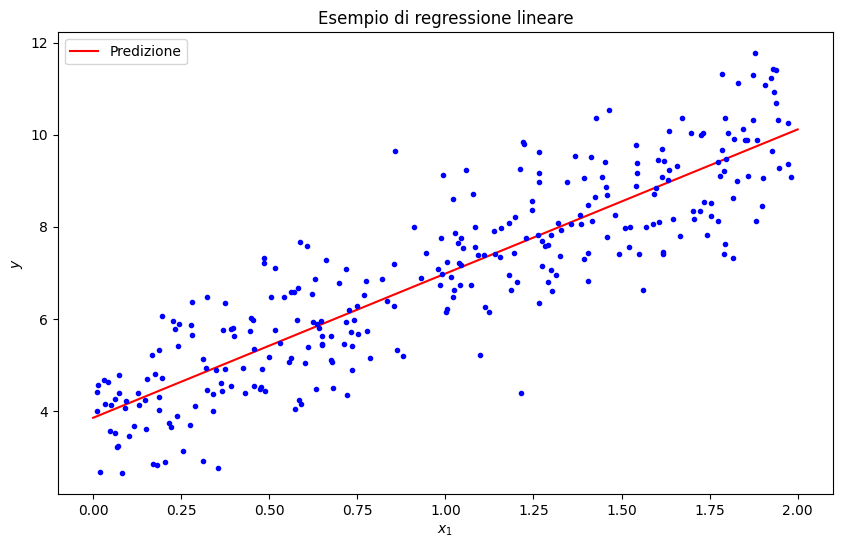
\includegraphics[width=0.8\textwidth]{images/regr_lin.png}
    \caption{Esempio di regressione lineare.}
    \label{fig:lin-reg}
\end{figure}



\subsection{Ricerca dei parametri: discesa del gradiente}
\label{gradiente}

Fino a questo momento abbiamo parlato di auto apprendimento della macchina in maniera del tutto generale, lasciando spazio alle ipotesi più fantasiose, fra cui l'idea che la macchina abbia un'effettiva intelligenza, simile a quella umana. In realtà, il modo in cui i sistemi auto apprendono è semplicemente quello di ricercare i parametri migliori (secondo quanto detto prima) per un determinato dominio applicativo. Ma come si trovano questi parametri? 
L'approccio più generale è chiamato \emph{discesa del gradiente} che non è altro che un algoritmo di ottimizzazione utilizzato per minimizzare una funzione obiettivo attraverso aggiornamenti iterativi. Nel nostro caso la funzione obbiettivo da minimizzare sarà ovviamente $E(\mathbf{\theta})$, cioè l'errore quadratico medio sulla predizione.
Essendo $E(\mathbf{\theta})$ una funzione, l'interpretazione geometrica di questo processo è di percorrere la curva lungo il punto in cui ha pendenza maggiore fino a trovare un minimo locale (o globale che sia).
Il vettore direzione che ci indica verso dove avanzare alle iterazioni successive è chiamato, appunto, \emph{gradiente}.
Dal punto di vista matematico, poiché l'errore è funzione di $\theta$, ovvero il vettore dei parametri dati alle variabili indipendenti, ci troveremo in uno spazio di $n+1$ dimensioni, dove $n$ corrisponde al numero di parametri. Supponendo di avere $n=2$ parametri graficamente avremo
le situazioni mostrate in figura \ref{fig:grad-descent}.
\begin{figure}
    \centering
    \begin{subfigure}[b]{0.48\textwidth}
        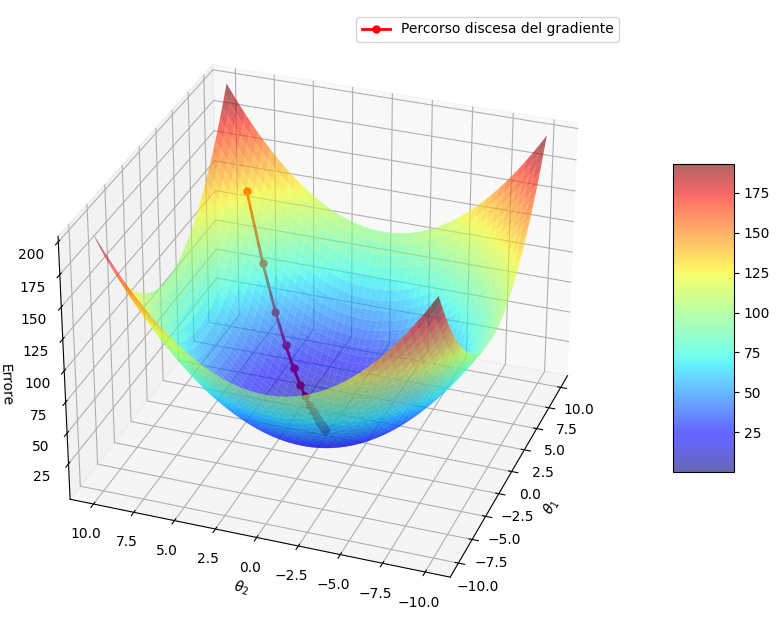
\includegraphics[width=\textwidth]{images/gradiente.png}
    \end{subfigure}
\quad
    \begin{subfigure}[b]{0.48\textwidth}
        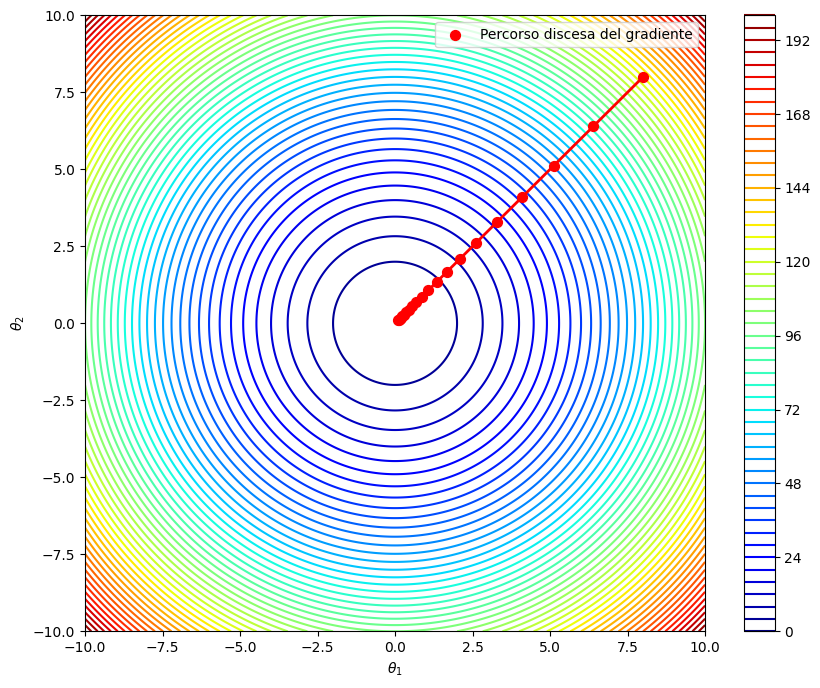
\includegraphics[width=\textwidth]{images/gradiente2.png}
    \end{subfigure}
    \caption{Rappresentazione grafica discesa del gradiente per un modello a due parametri.}
    \label{fig:grad-descent}
\end{figure}


Formalmente, il gradiente corrisponde al vettore delle derivate parziali della funzione errore rispetto a ogni parametro. Se si ha un solo parametro, il gradiente si identifica con la derivata della funzione errore. Dal punto di vista matematico le derivate forniscono la pendenza istantanea di una curva in un qualsiasi punto essa sia calcolata (ammesso che sia sempre derivabile, cosa vera per $E(\theta)$ essendo MSE). Perciò, muovendosi nella direzione opposta al gradiente, si procede nella maniera più efficiente possibile, poiché in tale direzione la funzione decresce al tasso più veloce.

Considerando $E(\theta)$ come la funzione da minimizzare, il suo gradiente si calcola come
\begin{align*}
    \nabla E(\theta) = \begin{bmatrix}
        \frac{\partial E}{\partial \theta_1} \\
        \frac{\partial E}{\partial \theta_2} \\
        \vdots \\
        \frac{\partial E}{\partial \theta_n}
    \end{bmatrix}
\end{align*}

A questo punto, per minimizzare $E$, aggiorniamo iterativamente il vettore dei parametri $\theta$ nella direzione opposta al gradiente. Definiamo come $\theta$ il vettore dei parametri all'iterazione precedente e $\theta'$ quello all'iterazione corrente. L'aggiornamento è dato da 
\begin{equation}\label{eq:discesa_gradiente}
    \theta' = \theta - \alpha \nabla E(\theta)
\end{equation}
dove $\alpha$ è un cosiddetto \emph{iperparametro}, ovvero un parametro con cui regolare le modalità in cui il modello apprende. Questo determina l'ampiezza da percorrere ad ogni iterazione. Un $\alpha$ troppo grande potrebbe far ``saltare'' il minimo, mentre uno troppo piccolo potrebbe rendere la convergenza troppo lenta.

Il processo si ripete fino al soddisfacimento di un \emph{criterio d'arresto}. Tale criterio può basarsi su diversi fattori:

\begin{itemize}
\item Arresto quando l'errore scende sotto una soglia predeterminata.
\item Arresto dopo un numero predefinito di iterazioni.
\end{itemize}


\subsection{Validazione del modello}
Per capire se il modello è effettivamente valido (da qui il nome \emph{validazione}) a descrivere un certo dominio applicativo si possono utilizzare due differenti approcci.
\begin{enumerate}
    \item Il metodo \emph{hold-out} rappresenta una delle strategie più elementari e diffuse per determinare l'efficacia di un modello di apprendimento automatico. Consiste essenzialmente nella suddivisione dell'insieme di dati in due segmenti distinti: uno dedicato all'addestramento del modello e l'altro alla sua validazione. Queste due porzioni sono frequentemente denominate \emph{train} e \emph{test} set.
    È usuale destinare tra il 70-80\% dell'insieme dei dati all'addestramento e il rimanente 20-30\% alla validazione, anche se tali percentuali possono essere adattate in base al contesto e alla mole di dati a disposizione.
    Il set di addestramento è impiegato per istruire il modello. Al termine di tale fase, il modello è sottoposto a verifica utilizzando il set di test. Poiché questi dati non sono stati utilizzati durante la fase di addestramento, consentono di valutare le capacità del modello nell'affrontare dati inediti.
    È inoltre praticabile una segmentazione ulteriore dell'insieme dei dati, introducendo un \emph{set di validazione}. Quest'ultimo è utilizzato per rifinire gli iperparametri del modello, mirando al miglioramento delle sue prestazioni. Conclusa questa ottimizzazione, il modello è nuovamente addestrato e, successivamente, la sua efficacia è testata con il set di test.
    È tuttavia essenziale considerare che l'affidabilità della valutazione potrebbe oscillare in base alla modalità di divisione dei dati. Se il set di test non risulta rappresentativo dell'intero insieme di dati, si potrebbero registrare incoerenze nella valutazione.
    \item La soluzione ai limiti dell'hold out arriva dalla \emph{$k-$fold cross validation} la quale mira a ottenere una valutazione più robusta e meno sensibile alle fluttuazioni che potrebbero derivare da una singola suddivisione casuale dei dati in set di addestramento e test, come avviene nel metodo hold-out. L'intero set di dati viene suddiviso in $k$ sottoinsiemi (o ``fold'') di dimensioni approssimativamente uguali. La procedura di addestramento e test viene ripetuta $k$ volte. Ogni volta, uno dei $k$ fold viene utilizzato come set di test, mentre gli altri $k-1$ fold vengono combinati per formare il set di addestramento. Pertanto, ogni dato nel set viene utilizzato esattamente una volta come dato di test. In questo modo l'errore finale è dato dalla somma degli errori di previsione sui singoli test. Questo fa si che l'errore trovato sia più generale e meno influenzato dai dati scegli per addestrarlo.
\end{enumerate}

Qualora a seguito della validazione del modello ci si rende conto che il modello non è in grado di generalizzare adeguatamente bene su nuovi dati non visti durante la fase di addestramento, possono presentarsi due problematiche (mostrate in Figura \ref{fig:over_under_fitting}).
\begin{enumerate}
    \item \emph{Underfitting}. Si verifica quando un modello è troppo semplice per catturare la struttura sottostante dei dati. Di conseguenza, il modello potrebbe avere una cattiva performance sia sul set di addestramento che sul set di test. Le ragioni per cui questo accade possono essere svariate, ma le più frequenti sono la scelta di un modello troppo semplice per descrivere le relazioni fra dati, la presenza di troppi pochi parametri o ancora l'addestramento effettuato per troppe poche iterazioni.
    \item \emph{Overfitting}. Si verifica quando un modello è troppo complesso e inizia a ``imparare'' anche il rumore presente nei dati di addestramento, anziché la struttura sottostante dei dati stessi. In pratica, un modello che soffre di overfitting avrà ottime prestazioni sul set di addestramento, ma avrà prestazioni scarse sul set di test o su nuovi dati non visti.
\end{enumerate}

Questo ci permette di capire che nel ML, di essenziale importanza è bilanciare la complessità del modello con la quantità e la qualità dei dati a disposizione, e monitorare attentamente le prestazioni del modello sia sul set di addestramento che sul set di test.


\begin{figure}
\centering
    \begin{subfigure}[b]{0.3\textwidth}
    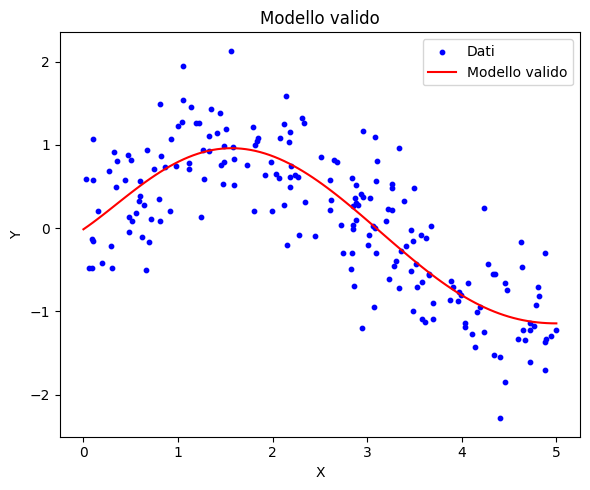
\includegraphics[width=\textwidth]{images/valido.png}
    \caption{Modello rappresentativo dei dati.}
    \end{subfigure}
\quad
    \begin{subfigure}[b]{0.3\textwidth}
    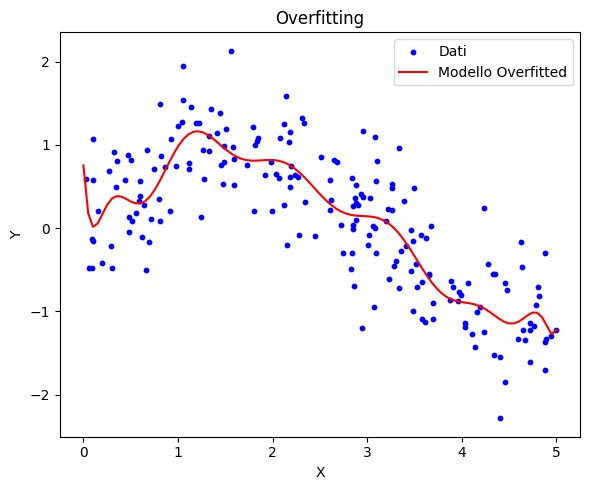
\includegraphics[width=\textwidth]{images/overfitting.png}
    \caption{Modello affetto da overfitting.}
    \end{subfigure}
\quad
    \begin{subfigure}[b]{0.3\textwidth}
    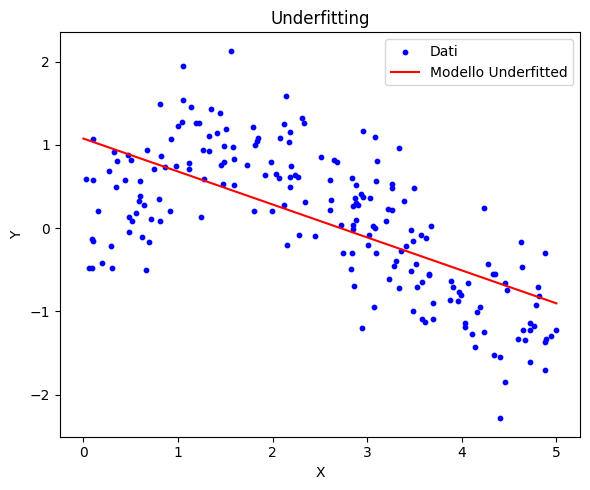
\includegraphics[width=\textwidth]{images/underfitting.png}
    \caption{Modello affetto da underfitting.}
    \end{subfigure}
\caption{}
\label{fig:over_under_fitting}
\end{figure}


\section{Reti Neurali}
Le \emph{reti neurali} rappresentano un pilastro centrale nel campo del machine learning. Sono modelli computazionali che traggono ispirazione dalla struttura e dalle funzionalità del cervello umano, progettati per replicare il modo in cui gli esseri umani apprendono e processano le informazioni. Il parallelo con il cervello umano, seppure non stretto, serve come modello concettuale per comprendere i principi di base del loro funzionamento.

\subsection{Struttura e Componenti di una Rete Neurale}
Le reti neurali sono formate da unità di calcolo denominate, appunto, \emph{neuroni} o \emph{nodi}, raggruppate in strati, o \emph{layers}. Questi si dividono in tre categorie principali:
\begin{itemize}
    \item \emph{Input layer}: rappresenta il punto di ingresso della rete, dove sono ricevuti gli input esterni.
    \item \emph{Hidden layers} (strati nascosti): possono essere plurimi e, più sono numerosi, più la rete è in grado di gestire complessità, migliorando le proprie performance. Qui, i dati in ingresso sono elaborati ulteriormente.
    \item \emph{Output layer}: è l'ultimo strato, attraverso il quale la rete fornisce i risultati dell'elaborazione dei dati in input.
\end{itemize}

\subsubsection{Funzionamento di un Neurone}
La Figura \ref{fig:neurone} illustra schematicamente il funzionamento di una singola unità neuronale. Ogni neurone riceve in input gli output di $n$ neuroni connessi a esso. Ogni connessione $i$ ha associato un \emph{peso} $w_i$, ottimizzato durante la fase di addestramento del modello. Il neurone moltiplica ogni input $x_i$ per il peso corrispondente, somma i prodotti ottenuti e aggiunge un \emph{bias} $b$ determinato anch'esso in fase di addestramento. Questa quantità è detta \emph{somma ponderata degli input}.
Questo bias è necessario per consentire al neurone di avere un grado di libertà aggiuntivo nel processo di apprendimento. Maggiore libertà comporta una maggiore adattabilità ai dati di addestramento.
Questa operazione produce la \emph{somma ponderata degli input}. Il bias fornisce al neurone un grado di libertà supplementare, permettendogli di adattarsi meglio ai dati durante la fase di apprendimento. La somma ponderata è poi processata da una \emph{funzione di attivazione} che decide se il neurone deve essere attivato o meno, introducendo una componente di \emph{non-linearità} essenziale per l'apprendimento di rappresentazioni complesse e relazioni non-lineari tra input e output. La formula appena descritta è la seguente:
\begin{equation*}
    \hat{y} = g(\mathbf{w \cdot x} + b) = g\left( \sum_{i=1}^n w_i \cdot x_i + b \right) 
\end{equation*}

\begin{figure}
    \centering
    \begin{tikzpicture}
        % Neuron
        \node[draw, circle, minimum size=1.5cm] (sum) at (0,0) {$\Sigma$};
        
        % Inputs
        \def\numInputs{4}
        \foreach \i in {1,2,...,\numInputs} {
            \ifnum\i=3
                \node at (-3, \numInputs - \i*1.5) {$\vdots$};
            \else
                \ifnum\i=4
                    \node[draw, circle, minimum size=0.5cm] (input\i) at (-3, \numInputs - \i*1.5) {$x_n$};
                    \draw[->] (input\i) -- (sum) node[midway, above] {$w_n$};
                \else
                    \node[draw, circle, minimum size=0.5cm] (input\i) at (-3, \numInputs - \i*1.5) {$x_\i$};
                    \draw[->] (input\i) -- (sum) node[midway, above] {$w_\i$};
                \fi
            \fi
        }
    
        % Bias
        \node[minimum size=0.5cm] (bias) at (0, 2.5) {$b$};
        \draw[->] (bias) -- (sum);
    
        % Activation
        \node[draw, circle, minimum size=1.5cm] (act) at (3, 0) {$g(\cdot)$};
        \draw[->] (sum) -- (act);
    
        % Output
        \node[minimum size=0.5cm] (output) at (6, 0) {$\hat{y}$};
        \draw[->] (act) -- (output);    
    
    \end{tikzpicture}
    \caption{Schema di funzionamento unità neuronale.}
    \label{fig:neurone}
\end{figure}

\subsubsection{Funzioni di Attivazione}
Le funzioni di attivazione si classificano principalmente in due categorie, in base al loro codominio: 
\begin{itemize}
    \item \emph{Funzioni di attivazione normalizzate}: queste funzioni, ad esempio, mappano i reali in intervalli del tipo $[0,1]$ o $[-1, 1]$, risultando particolarmente utili nei layer di output quando la rete deve produrre probabilità, come nei task di classificazione. Alcuni esempi includono:
    \begin{itemize}
        \item \emph{Sigmoide}. Può essere utile nella classificazione binaria poiché è definita in $\mathbb{R} \rightarrow [0,1]$. Si ottiene con
        \begin{equation*}
            \sigma(x) = \frac{1}{1+e^{-x}}
        \end{equation*}
        \item \emph{Tangente iperbolica}. Definita in $\mathbb{R} \rightarrow [-1,1]$ e vale
        \begin{equation*}
            \tanh(x) = \frac{2}{1+e^{-2x}} - 1
        \end{equation*}
    \end{itemize}
    \item \emph{Funzioni di attivazione continue}: queste mappano  $\mathbb{R} \rightarrow \mathbb{R}$. e l'output determina non solo se il neurone è attivato, ma anche la quantità di segnale trasmesso. Un esempio noto è la \emph{ReLU} (Rectified Linear Unit) ed è definita in $\mathbb{R} \rightarrow \mathbb{R}^+$. Se si attiva trasmette un segnale proporzionale alla somma pesata degli input, infatti è definita come
    \begin{equation*}
        \text{ReLU}(x) = \text{max}(0, x)
    \end{equation*}
    Se l'input ($x$) è negativo, il neurone restituisce 0, interpretato come uno ``spegnimento'' del neurone; se positivo, il neurone restituisce l'input ricevuto.
\end{itemize}

\subsection{Processo di Addestramento}
Durante l'addestramento di una rete neurale, come precedentemente menzionato, si scelgono i pesi delle connessioni tra neuroni e i bias di questi, in modo da rappresentare al meglio i dati di esempio. Analogamente agli algoritmi di Machine Learning (ML) tradizionali, l'accuratezza del modello viene valutata mediante una funzione d'errore, nota come \emph{loss function}, che quantifica la divergenza del modello dalla soluzione desiderata. Il valore ottenuto, frequentemente denominato perdita'' o errore'', è indicativo dell'accuratezza del modello: valori bassi sono indice di predizioni precise, mentre valori alti denotano predizioni inesatte. L'obiettivo durante la fase di addestramento è minimizzare il valore della funzione di perdita.
Per ridurre la loss, si adotta l'approccio della discesa del gradiente (vedi paragrafo \ref{gradiente}). In particolare, ad ogni iterazione, comunemente definita come \emph{``epoca di addestramento''} nel contesto delle reti neurali, si procede attraverso i seguenti passaggi:
\begin{itemize}
\item Si effettuano predizioni sui dati di esempio basandosi sui parametri attuali del modello.
\item Si calcola la loss confrontando le predizioni con i valori reali.
\item Si determina il gradiente della funzione di perdita rispetto ai parametri attuali del modello.
\item Si aggiornano i parametri del modello muovendosi nella direzione che minimizza la funzione di perdita, come descritto dall'equazione \ref{eq:discesa_gradiente}.
\end{itemize}

\subsection{Reti Neurali Feed-forward (FNN)}
Le reti neurali di tipo \emph{feedforward}, quali ad esempio i Multilayer Perceptron, rappresentano le forme più elementari e fondamentali di reti neurali. Questi modelli sono caratterizzati da un flusso d’informazione che procede in un’unica direzione, andando dal layer di input, passando per gli eventuali layer nascosti, fino a raggiungere il layer di output. In queste strutture, il processo attraverso il quale l’informazione è inviata da un neurone all’altro è conosciuto come \emph{forwarding}.
Nel dettaglio, in un'architettura feedforward, ogni neurone è interconnesso con tutti i neuroni presenti nel layer immediatamente successivo, formando una rete densamente connessa in cui l'informazione si muove in modo ordinato e strutturato da uno strato all'altro, senza cicli o ritorni. Questa struttura rigidamente organizzata si contrappone a modelli più complessi, come le reti \emph{neurali ricorrenti} (trattate nel paragrafo successivo), che permettono connessioni in entrata anche da neuroni situati nello stesso layer o in layer successivi.
Analizzando più profondamente il funzionamento di ogni singolo neurone, come illustrato nella Figura \ref{fig:neurone}, è possibile notare che tutti gli input ricevuti da un neurone provengono esclusivamente da neuroni situati nel layer precedente, e ogni output prodotto è destinato unicamente ai neuroni del layer successivo. Ciò implica che ogni neurone opera come una sorta di stazione di transito, ricevendo segnali in ingresso, elaborandoli e inoltrandoli ai neuroni successivi, contribuendo così alla progressiva trasformazione dell'input iniziale fino all'ottenimento dell'output finale.
Nelle reti neurali feedforward, i layer nascosti hanno il compito di elaborare e trasformare progressivamente le informazioni in ingresso, estraendo e combinando caratteristiche e rappresentazioni ad alto livello, indispensabili per l'esecuzione di compiti complessi. La presenza di più layer nascosti, ciascuno con un numero variabile di neuroni, consente alla rete di modellare relazioni e pattern sempre più complessi e astratti, aumentando la sua capacità di apprendimento e generalizzazione.
La Figura \ref{fig:fnn} mostra un esempio di rete neurale feedforward, composta da un layer di input, tre layer nascosti e un layer di output. In questa rappresentazione grafica, è possibile osservare la strutturazione gerarchica e sequenziale della rete e l'organizzazione delle connessioni tra i diversi neuroni, che evidenzia la natura unidirezionale e strutturata del flusso informativo all'interno del modello.


\begin{figure}
    \centering
    \begin{tikzpicture}[>=stealth, neuron/.style={circle, draw, minimum size=0.5cm}, font=\footnotesize]

        % Neuroni
        \foreach \i in {1,...,7} \node[neuron] (I-\i) at (0,\i) {};
        \foreach \i in {1,...,5} \node[neuron] (H1-\i) at (2.5,\i + 1) {};
        \foreach \i in {1,...,3} \node[neuron] (H2-\i) at (5,\i + 2) {}; 
        \foreach \i in {1,...,5} \node[neuron] (H3-\i) at (7.5,\i + 1) {};
        \foreach \i in {1,...,3} \node[neuron] (O-\i) at (10,\i + 2) {}; 
        
        % Connetti neuroni
        \foreach \i in {1,...,7} \foreach \j in {1,...,5} \draw[->] (I-\i) -- (H1-\j);
        \foreach \i in {1,...,5} \foreach \j in {1,...,3} \draw[->] (H1-\i) -- (H2-\j);
        \foreach \i in {1,...,3} \foreach \j in {1,...,5} \draw[->] (H2-\i) -- (H3-\j);
        \foreach \i in {1,...,5} \foreach \j in {1,...,3} \draw[->] (H3-\i) -- (O-\j);
        
        % Nodi titoli dei layer
        \node[below=of I-4, yshift=-2cm] (IL) {Input Layer}; 
        \node[below=of H1-3, yshift=-2cm] (H1L) {Hidden Layer 1};
        \node[below=of H2-2, yshift=-2cm] (H2L) {Hidden Layer 2};
        \node[below=of H3-3, yshift=-2cm] (H3L) {Hidden Layer 3};
        \node[below=of O-2, yshift=-2cm] (OL) {Output Layer};
    
    \end{tikzpicture}
    \caption{Feedforward Neural Network.}
    \label{fig:fnn}
\end{figure}



\subsection{Reti Neurali Ricorrenti (RNN)}
\label{rnn}
Le \emph{reti neurali ricorrenti} (RNN) sono una classe speciale di reti neurali che sono particolarmente efficaci nel trattare sequenze di dati, come serie temporali o sequenze di testo. A differenza delle reti neurali feedforward (FNN), le RNN sono in grado di mantenere uno stato interno che cattura le informazioni relative alle parti precedenti della sequenza.
In particolare le FNN presentano limitazioni significative quando si tratta di elaborare dati sequenziali o temporali (si pensi ad esempio a tutti quei task che coinvolgono testo dove per comprendere una frase è necessario avere contezza del significato delle parole precedenti in relazione a quella attuale). In particolare
\begin{itemize}
    \item \emph{Mancanza di memoria temporale}. Le FNN non hanno memoria interna o stato che può catturare l'ordine o la sequenza delle informazioni, rendendole inefficienti per problemi che richiedono la considerazione del contesto temporale o sequenziale. Le informazioni fluiscono senza lasciare traccia all'interno della rete. Ogni input è considerato a se stante. 
    \item \emph{Dimensione fissa dell'input}. Le FNN richiedono che l'input sia di dimensione fissa, il che è limitante per l'elaborazione di sequenze di lunghezza variabile. Infatti, come mostra Figura \ref{fig:fnn}, quando si definisce l'architettura di una rete feedforward, si specifica il numero di neuroni in ogni layer, e quindi il numero di pesi in ogni layer è fisso una volta definita l'architettura. 
    \item \emph{Indipendenza delle feature}. Le FNN assumono che tutte le feature di input siano indipendenti l'una dall'altra, il che non è ideale per i dati sequenziali in cui l'ordine e il contesto delle informazioni sono cruciali.
\end{itemize}
Al contrario, le RNN, nascono con l'obbiettivo di superare questi limiti. Esse sono infatti capaci di \emph{mantenere uno stato} e gestire sequenze di \emph{dimensione variabile} di input/output.

Tutta la potenzialità di queste reti si basa su un principio molto semplice: piuttosto che usare i neuroni come aree di transito dell'informazione, può essere utile che ognuno di essi abbia la possibilità di mantenere in memoria uno \emph{stato nascosto} (hidden state) che si aggiorni ad ogni nuova informazione in arrivo e che venga propagato assieme ad essa ai neuroni successivi. 
Questo permette alla rete di mantenere informazioni relative ai passaggi precedenti della sequenza mentre elabora ogni nuovo elemento. Potremmo in altre parole vedere questo stato come una ``memoria'' della rete.
Questi stati nascosti vengono generati da delle \emph{connessioni ricorrenti}, ovvero archi che formano cicli all'interno della rete: piuttosto che confluire in un'unica direzione, l'informazione può tornare anche indietro nella rete, per questo motivo si parla di \emph{backpropagation}.
In definitiva l'output di una rete neurale ricorrente è funzione sia del suo hidden state che dell'input fornito.

Formalmente coccorre immaginare che le informazioni vengano processate ad intervalli discreti di tempo $t_0 \rightarrow t_1 \rightarrow t_2 \rightarrow \cdots$.
Ad ogni iterazione $t_i$ il vettore di stato nascosto viene aggiornato (dopo che l'informazione è processata all'interno di un ciclo, o connessione ricorrente) mantenendo ``in memoria'' tutta la sequenza di input fino a quel momento. Durante la fase di \emph{forwardpropagation} il neurone invia, oltre all'input arrivato al tempo $t_i$ il suo stato nascosto aggiornato al passo $t_{i-1}$. 

\subsubsection{Reti di Elman}
Le \emph{reti neurali di Elman} sono il caso più semplice di RNN e dunque si prestano bene per comprendere il concetto di hidden state e connessioni ricorrenti.
Una rete di Elman è molto simile ad una rete neurale feedforward a singolo strato nascosto, ma nello strato nascosto viene aggiunto un insieme di neuroni detti \emph{unità di contesto}.
In questo tipo di rete il comportamento appena descritto si ottiene in questo modo: per ogni neurone presente nello strato nascosto
si aggiunge un’unità neuronale detta \emph{di contesto} che riceve come input l’output del neurone nascosto corrispondente, e restituisce il proprio output allo stesso neurone.
nascosto.

In altre parole la funzione \ref{eq:rel_modello}, viene aggiornata nel seguente modo all'interno delle reti di Elman

\begin{equation*} %correggi la formula per essere aderente alla rappr. grafica
    \hat{y}_t = g(\mathbf{w} \cdot \mathbf{x}_t + \mathbf{u} \cdot \mathbf{h}_{t-1} + b)
\end{equation*}

La Figura \ref{fig:elmanrnn} mostra come sono strutturate questo tipo di reti.


\begin{figure}
    \centering
    \begin{tikzpicture}[>=stealth, neuron/.style={circle, draw, minimum size=0.5cm}, font=\footnotesize]

        % Neuroni
        \node[neuron] (I-1) at (0,6) {$x_1$};
        \node[neuron] (I-2) at (0,4) {$x_2$};
        \node[neuron] (I-3) at (0,1) {$x_k$}; 
        
        \node[neuron] (H-1) at (4,6) {$h_1$};
        \node[neuron] (H-2) at (4,4) {$h_2$};
        \node[neuron] (H-3) at (4,1) {$h_l$};
        
        \node[neuron] (O-1) at (8,6) {$o_1$};
        \node[neuron] (O-2) at (8,4) {$o_2$};
        \node[neuron] (O-3) at (8,1) {$o_n$}; 

        \node[neuron] (U-1) at (4,-1) {$u_1$};
        \node[neuron] (U-2) at (4,-3) {$u_2$};
        \node[neuron] (U-3) at (4,-6) {$u_l$};

        \node (y-1) at (10,6) {$y_1$};
        \node (y-2) at (10,4) {$y_2$};
        \node (y-3) at (10,1) {$y_n$};
        
        % Vdots
        \node at (0,2.5) {$\vdots$}; 
        \node at (4,2.5) {$\vdots$}; 
        \node at (8,2.5) {$\vdots$}; 
        \node at (4,-4.5) {$\vdots$};
        \node at (10, 2.5) {$\vdots$};
        
        % Connetti neuroni
        \foreach \i in {1,2,3} \foreach \j in {1,2,3} \draw[->] (I-\i) -- (H-\j);
        \foreach \i in {1,2,3} \foreach \j in {1,2,3} \draw[->] (H-\i) -- (O-\j);
        \draw[->] (U-1) to [out=180,in=180,looseness=0.75] (H-1);
        \draw[->] (H-1) to [out=0,in=0,looseness=0.75] (U-1);
        \draw[->] (U-2) to [out=180,in=180,looseness=0.75] (H-2);
        \draw[->] (H-2) to [out=0,in=0,looseness=0.75] (U-2);
        \draw[->] (U-3) to [out=180,in=180,looseness=0.75] (H-3);
        \draw[->] (H-3) to [out=0,in=0,looseness=0.75] (U-3);
        
        \draw (-1,6) -- (I-1) node[midway, above] {$in_1$};
        \draw (-1,4) -- (I-2) node[midway, above] {$in_2$};
        \draw (-1,1) -- (I-3) node[midway, above] {$in_k$};

        \draw[->] (O-1) -- (y-1);
        \draw[->] (O-2) -- (y-2);
        \draw[->] (O-3) -- (y-3);
    \end{tikzpicture}
    \caption{Rete neurale ricorrente di Elman.}
    \label{fig:elmanrnn}
\end{figure}




\section{Natural Language Processing}
L'elaborazione del linguaggio naturale (NLP, \emph{Natural Language Processing}) è un campo interdisciplinare che combina linguistica, informatica e intelligenza artificiale, con l'obiettivo di permettere alle macchine di interpretare, comprendere e generare il linguaggio umano. Il linguaggio naturale è estremamente complesso e ricco di sfumature, implicazioni e ambiguità, il che rende il NLP una sfida difficile e al contempo estremamente affascinante.


\subsection{Complessità del linguaggio naturale}
Come già anticipato, il linguaggio naturale è intrinsecamente ambiguo e polisemico, ovvero una stessa parola può avere significati diversi a seconda del contesto in cui è inserita. Inoltre, il linguaggio è ricco di espressioni idiomatiche, metafore, sarcasmo e humor, che possono essere difficili da interpretare anche per gli esseri umani, figuriamoci per un calcolatore. Anche la struttura grammaticale e sintattica può variare enormemente tra lingue diverse, con differenze in ordine delle parole, morfologia, e costruzione delle frasi.
A tutto questo si aggiungono anche la possibilità di abbreviare parole o intere frasi e di commettere errori sintattici o lessicali.

\subsection{Sfide principali}
In questo contesto così complicato e affascinante spiccano una serie di task ad oggi di particolare interesse. 
\begin{itemize}
    \item \emph{Disambiguazione semantica delle parole} (WSD). Determinare il significato appropriato di una parola in un determinato contesto è una sfida fondamentale in NLP, data la presenza di parole identiche ma con significati diversi in base al contesto.
    Un esempio potrebbe essere il seguente
    \begin{center}
        ``Conseguire un titolo di studio avanzato è considerato un obiettivo \emph{ambito} nel mondo accademico.'' \\
        oppure \\
        ``L'\emph{ambito} del Natural Language Processing è estremamente affascinante''.
    \end{center}
    Nelle due frasi il significato di \emph{ambito} cambia totalmente.
    \item \emph{Analisi del sentimento}. Comprendere il sentimento o il tono emotivo dietro una frase è cruciale in molte applicazioni, come il monitoraggio dei social media o la valutazione delle recensioni dei prodotti. 
    \begin{center}
        ``Il nuovo design di VirtuaLe mi piace'' $\rightarrow$ Positiva. \\
        ``Non so se il nuovo design di VirtuaLe mi piace'' $\rightarrow$ Neutra. \\
        ``Il nuovo design di VirtuaLe non mi piace'' $\rightarrow$ Negativa. 
    \end{center}
    \item \emph{Generazione di testo}. Creare testo coerente, grammaticalmente corretto e semanticamente sensato è un'importante sfida, utile in applicazioni come i chatbot e la creazione di contenuti.
    \item \emph{Summarization}. Riguarda la produzione di una rappresentazione concisa delle informazioni principali contenute in un testo più esteso. L'obiettivo è di mantenere il significato e le informazioni cruciali del testo originale, riducendone però la lunghezza. Questo task è oggetto del seguente progetto di tesi.
\end{itemize}

\subsubsection{Summarization estrattiva e astrattiva}
Come accennato in precedenza, il task di summarization implica la creazione di una rappresentazione sintetica delle informazioni contenute in un documento più ampio, mantenendo inalterato il suo significato originale. Questa sfida, oltre ad essere di grande interesse, è di fondamentale importanza per fornire agli utenti un assaggio di un documento, un articolo, una notizia o qualsiasi altro tipo di testo, permettendo loro di comprendere i punti chiave senza dover leggere l'intero contenuto.

Esistono principalmente due modalità di summarization: \emph{extractive} e \emph{abstractive}.
Più nel dettaglio:
\begin{itemize}
\item \emph{Extractive Summarization}. Questa metodologia crea riassunti individuando e estraendo le frasi o i segmenti di testo più significativi e informativi dal documento originale. Non viene creato nuovo testo, bensì vengono scelte porzioni del documento originale. Ciò richiede una significativa capacità di comprensione del testo per selezionare le sezioni più pertinenti, ma è meno esigente rispetto ai modelli abstrattivi.
Gli algoritmi di extractive summarization frequentemente adoperano tecniche quali la pesatura delle parole, la posizione delle frasi nel documento, e la co-occorrenza di termini, che analizza la frequenza con cui parole o termini appaiono insieme in un determinato contesto, come un documento o una finestra di parole nel testo.
\item \emph{Abstractive Summarization}. Al contrario dell'approccio estrattivo, l'abstractive summarization produce nuove frasi che sintetizzano il contenuto principale del documento. Questo metodo necessita di una comprensione più profonda del testo e dell'abilità di riformulare concetti con nuove parole. Gli algoritmi di abstractive summarization fanno spesso ricorso a tecniche avanzate di deep learning, come i modelli di \emph{attention} e i \emph{Transformer} (discussi nei successivi paragrafi), per creare riassunti più coerenti e fluidi.
\end{itemize}

Come suggerisce il titolo di questa tesi, per i nostri esperimenti abbiamo deciso di utilizzare i modelli astrattivi disponibili in letteratura, piuttosto che tentare approcci estrattivi. 
Dato che l'obiettivo, come delineato nell'introduzione, è la generazione di riassunti lay, ovvero formulati in modo meno tecnico e più accessibile ad un ampio pubblico, il task ha portato con sé ulteriori sfide, quali l'identificazione delle sezioni cruciali del testo e la loro semplificazione. Per questa ragione, si è ritenuto che gli approcci extractive non fossero adeguatamente efficaci per raggiungere tale scopo.


\subsection{Pre-processing di testo} 
\label{preproc}
Tutte le problematiche intrinseche del linguaggio delineate in precedenza vengono parzialmente arginate da una fase preliminare chiamata \emph{pre-processing}. 
Il preprocessing del testo è un passaggio cruciale nell'ambito del Natural Language Processing (NLP), il quale mira a semplificare il testo e ridurre la sua complessità, permettendo ai modelli di apprendimento automatico di operare più efficacemente.
Ovviamente nel corso del tempo sono state introdotte un numero cospiquo di tecniche di questo tipo, ma le più importanti sono le seguenti

\begin{itemize}
    \item \emph{Tokenizzazione}. La tokenizzazione è un passaggio cruciale nel pre-processing del testo per il Natural Language Processing (NLP). Questo processo consiste nella suddivisione del testo in ingresso (corpus) in unità più piccole e maneggevoli, denominate ``\emph{token}''. Questi token rappresentano spesso parole, ma possono anche rappresentare simboli, frasi o altre unità di testo, a seconda delle specifiche necessità del task di NLP in questione. La tokenizzazione è essenziale per convertire il linguaggio naturale in una forma che può essere interpretata e manipolata dai modelli di machine learning, trasformando il testo grezzo in una struttura di dati più organizzata, come un vettore di token. Questo passo preliminare permette di preparare il testo per le successive fasi di elaborazione, come la vettorializzazione. 
    \item \emph{Rimozione delle Stop Words}. Nel linguaggio naturale esistono parole che non apportano alcun contributo al contenuto del testo, ma servono solamente ad arricchire il linguaggio e permettere una comprensione migliore a coloro che leggono. Esse sono parole funzionali che servono a collegare le parole contentive, cioè quelle che trasportano il significato principale del discorso, e a strutturare grammaticalmente le frasi. Senza le stop word, il linguaggio sarebbe frammentario e privo di coesione, rendendo difficile la comprensione del discorso. Per loro natura, dunque, non contribuiscono a dare significato al testo e pertanto non solo risultano inutili alla comprensione del testo da parte di un modello di NLP, ma aumentano la dimensionalità del problema rendendo più difficile e lungo l'addestramento. Alcuni esempi di queste parole possono essere ad esempio le congiunzioni come ``e'', ``di'', ``in'', ecc.  
    \item \emph{Lemmatizzazione e Stemming}. La lemmatizzazione e lo stemming sono tecniche di elaborazione del linguaggio naturale che mirano a ridurre le parole a una forma base o radice, facilitando così l'analisi del testo e migliorando l'efficacia dei modelli di NLP. In particolare 
    \begin{itemize}
        \item La lemmatizzazione è il processo di riduzione di una parola alla sua forma canonica o lemma, cioè alla sua forma base che ha un significato nel dizionario. Questo processo tiene conto del contesto e della morfologia della parola, utilizzando vocabolari e analisi grammaticali per assicurare che la parola risultante abbia un significato valido. 
        \item Lo stemming, a differenza della lemmatizzazione, è un processo più rudimentale che riduce le parole alla loro radice tramite regole euristico-morfologiche, senza tenere conto del contesto. Questo processo può talvolta produrre radici che non hanno un significato valido nel dizionario. 
        Sebbene potrebbe sembrare una pratica meno valida della lemmatizzazione in quanto può produrre parole prive di significato, tuttavia, poiché si tratta solamente di troncare la parola alla sua radice, il processo è estremamente pià efficiente e pertanto adatto a grandi moli di dati.
    \end{itemize}
    Entrambe le tecniche sono molto utili per ridurre la dimensionalità del corpus, in quanto tutte le parole derivate si riducono alla loro forma base in un caso e alla loro radice nell'altra.
    \item \emph{Normalizzazione del Testo}. Riguarda la conversione del testo in una forma standard e uniforme, tipicamente rendendo minuscole tutte le lettere del testo. Questo può aiutare a migliorare le performance del modello.
    \item \emph{Tagging Part-of-Speech}. Un modo per disambiguare, quanto meno in parte, il significato delle parole all'interno del testo è attribuire a ciascuna di esse un ruolotradeoff grammaticale all'interno delle varie frasi. Più nel dettaglio consiste nell'etichettare ogni parola in una frase con la sua parte del discorso grammaticale, come sostantivo, verbo, aggettivo, avverbio, ecc. Questo processo è essenziale per comprendere la struttura grammaticale delle frasi e per analizzare le relazioni semantiche tra le parole.
    \item \emph{Creazione di N-grammi}. Non è sempre possibile attribuire un significato autonomo a ogni parola all'interno di un testo. Esistono infatti termini composti, come ``New York'', che possono essere frazionati in modo errato durante la tokenizzazione. Per ovviare a questo inconveniente, è possibile ricorrere alla creazione di $n$-gram, ossia tuple composte da $n$ parole consecutive, con $n$ arbitrario. È importante sottolineare che, all'aumentare di $n$, la probabilità di formare combinazioni di parole coerenti e sensate tende a diminuire significativamente.
    Le modalità di POS tagging sono molteplici fra cui approcci statistici e modelli di RNN addestrati a capire le relazioni fra parole su centinaia di migliaia di frasi annotate.
    \item \emph{Rappresentazione Vettoriale (Vectorization)}. La vettorializzazione dei token è un processo cruciale che converte parole, frasi o documenti, rappresentati come token, in vettori di numeri. Questo processo è fondamentale poiché i modelli di machine learning e le tecniche di analisi dei dati possono lavorare efficacemente solo con dati numerici. La rappresentazione vettoriale permette di quantificare e analizzare il testo in modo che i modelli di apprendimento possano comprenderlo e processarlo. Esistono diverse strategie per la vettorializzazione, che spaziano da metodi più semplici, come il modello \emph{Bag-of-Words (BoW)}, dove il documento è descritto come un vettore le cui componenti rappresentano la frequenza delle parole nel documento, a metodi più sofisticati come i \emph{Word Embeddings}. In questo caso esistono molti algoritmi, fra cui \emph{Word2Vec}\cite{mikolov2013efficient} e \emph{GloVe}\cite{pennington-etal-2014-glove}, tutti quanti accumunati dal concetto di rappresentare le parole come vettori densi in uno spazio vettoriale continuo. In questo modo si è in grado di catturare la semantica delle parole, consentendo a parole semanticamente simili di avere vettori simili, graficamente questo è mostrato in Figura \ref{fig:word-embeddings}. 

    L'utilizzo di tali rappresentazioni vettoriali offre il considerevole vantaggio di poter applicare operazioni matematiche ai vettori, ottenendo risultati semanticamente coerenti nelle parole corrispondenti. Alcuni esempi celebri di questa proprietà sono dati dalle seguenti operazioni vettoriali:

    \begin{align*}
        \text{King} - \text{Man} + \text{Woman} &= \text{Queen} \\
        \text{Human} - \text{Animal} &= \text{Ethics}
    \end{align*}

    In questo modo, il modello può effettivamente ``ragionare'' in termini semanticamente significativi, aprendo nuove possibilità nella modellazione del linguaggio naturale e nell'analisi del testo.
    
\end{itemize}

\begin{figure}
    \centering
    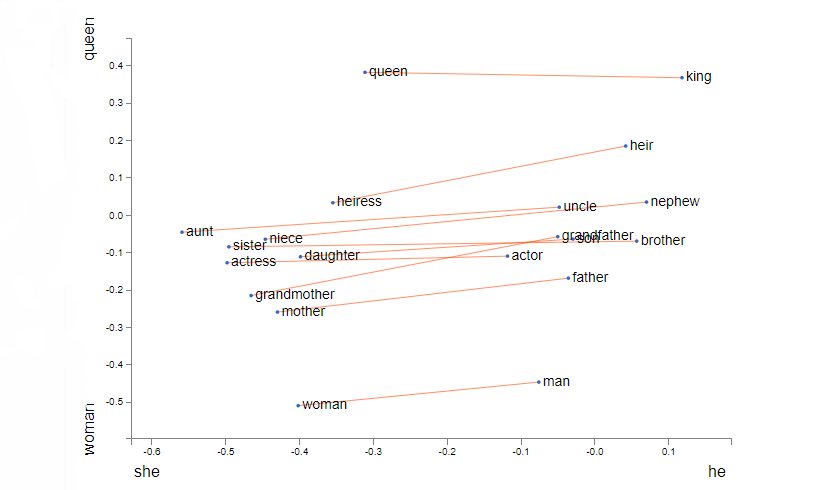
\includegraphics[width=\textwidth]{images/word2vec-example.png}
    \caption{Proiezioni di parole su spazio vettoriale $\mathbb{R}^2$.}
    \tiny{Fonte: https://lamyiowce.github.io/word2viz/}
    \label{fig:word-embeddings}
\end{figure}

\section{Tecniche astrattive allo stato dell'arte}
Alcune delle architetture più avanzate, tecnicamente definite \emph{allo stato dell'arte}, per compiti quali la generazione di testo, la comprensione del linguaggio e la traduzione, come i seguenti Large Language Models (LLMs) \emph{BART} \cite{DBLP:journals/corr/abs-1910-13461}, \emph{GPT-3} \cite{DBLP:journals/corr/abs-2005-14165}, e \emph{T5} \cite{DBLP:journals/corr/abs-1910-10683}, si basano sulle tecniche introdotte di seguito fra cui spiccano
\begin{itemize}
    \item Modelli \emph{Sequence-to-Sequence}.
    \item Meccanismo di \emph{Attention}.
    \item Architettura a \emph{Transformers}.
\end{itemize}

\subsection{Modelli Seq2Seq}
I modelli \emph{Seq2Seq} (Sequence-to-Sequence) sono un tipo di architettura di rete neurale utilizzata per la generazione di sequenze, in cui una rete prende in input una sequenza e produce in output un'altra sequenza. Questo tipo di modelli è stato ampiamente utilizzato in una varietà di applicazioni, tra cui la traduzione automatica, la generazione di testo, la sintesi vocale e molto altro, nella pubblicazione originale \cite{cho2014learning} erano basati su RNN, ma con il passare del tempo si sono evoluti fino a portare, come anticipato, alle architetture più moderne che fanno uso di transformers e self-attention.

\subsubsection{Funzionamento}
Come suggerisce il nome, seq2seq è un modello che prende in input una sequenza di oggetti (parole, lettere, pixel di un'immagine, ecc.) e restituisce in output una nuova sequenza di oggetti, tipicamente correlati in qualche modo ai primi. Ad esempio se si stesse implementato un modello di traduzione, l'input sarebbe una frase in una lingua e l'ouput sarebbe la sua traduzione in un'altra.

Come mostra la Figura \ref{fig:seq2seq}, questi modelli sono composti da due componenti
\begin{itemize}
    \item \emph{Encoder}. Questa prima parte si occupa di processare ciascun elemento nella sequenza di input, generare un vettore chiamato \emph{context}, che catturi le informazioni della sequenza, e di spedirlo al \emph{decoder}.
    \item \emph{Decoder}. Posto a cascata dopo l'encoder, questo si occupa, una volta che il primo gli ha inviato il context, di produrre la nuova sequenza di output elemento per elemento, esattamente come l'encoder ha consumato quella in input.
\end{itemize}




\begin{figure}
\centering
    \begin{subfigure}[b]{\textwidth}
        \centering
            \begin{tikzpicture}[>=Stealth, node distance=1cm, thick,
            container/.style={draw, rectangle, inner sep=0.2cm, align=center},
            bigbox/.style={draw, rectangle, minimum height=2.5cm, minimum width=6cm, align=center},
            box/.style={draw, rectangle, minimum height=2.3cm, minimum width=2.2cm, align=center},
            context/.style={draw, rectangle, minimum height=0.4cm, minimum width=2.1cm, align=center}]
            \tikzstyle{input_node}=[inner sep=0pt, outer sep=0pt]
            % Triangle vector
            \node [container, label=above:Input Vector] (tContainer) {
                \begin{tikzpicture}
                    \node [input_node] (t1) {Io};
                    \node [input_node, right=0.2cm of t1] (t2) {sono};
                    \node [input_node, right=0.2cm of t2] (t3) {uno};
                    \node [input_node, right=0.2cm of t3] (t4) {studente};
                \end{tikzpicture}
            };
            
            % Big Box
            \node [bigbox, label=above:Seq2Seq model, right=1cm of tContainer] (bigbox) {};
            \node [box, left=0.7cm of bigbox.center] (encoder) {Encoder};
            \node [box, right=0.7cm of bigbox.center] (decoder) {Decoder};
            
            
            % Arrows
            \draw [->] (tContainer) -- (bigbox);
            \end{tikzpicture}
        \caption{Ingresso delle parole all'interno dell'encoder.}
    \end{subfigure}
    
    \vspace{\baselineskip} 
    
    \begin{subfigure}[b]{\textwidth}
        \centering
            \begin{tikzpicture}[>=Stealth, node distance=1cm, thick,
            container/.style={draw, rectangle, inner sep=0.2cm, align=center},
            bigbox/.style={draw, rectangle, minimum height=2.5cm, minimum width=6cm, align=center},
            box/.style={draw, rectangle, minimum height=2.3cm, minimum width=2.2cm, align=center},
            context/.style={draw, rectangle, minimum height=0.4cm, minimum width=2.1cm, align=center}]
            \tikzstyle{input_node}=[inner sep=0pt, outer sep=0pt]
            
            % Big Box
            \node [bigbox, label=above:Seq2Seq model, right=1cm of tContainer] (bigbox) {};
            \node [box, left=0.7cm of bigbox.center] (encoder) {Encoder};
            \node [box, right=0.7cm of bigbox.center] (decoder) {Decoder};
            
            % Context positioned above the arrow
            \node [context, rotate=90, at=(bigbox.center)] (context) {Context};

            % Arrows
            \draw [->] ([yshift=-1.1cm]encoder.east) -- ([yshift=-1.1cm]decoder.west);
            \end{tikzpicture}
        \caption{Creazione e forwarding del context vector.}
    \end{subfigure}
    
    \vspace{\baselineskip} % O qualche altro spazio verticale che preferisci
    
    \begin{subfigure}[b]{\textwidth}
        \centering
        \begin{tikzpicture}[>=Stealth, node distance=1cm, thick,
        container/.style={draw, rectangle, inner sep=0.2cm, align=center},
        bigbox/.style={draw, rectangle, minimum height=2.5cm, minimum width=6cm, align=center},
        box/.style={draw, rectangle, minimum height=2.3cm, minimum width=2.2cm, align=center},
        context/.style={draw, rectangle, minimum height=0.4cm, minimum width=2.1cm, align=center}]
        \tikzstyle{input_node}=[inner sep=0pt, outer sep=0pt]
        
        % Big Box
        \node [bigbox, label=above:Seq2Seq model, right=1cm of tContainer] (bigbox) {};
        \node [box, left=0.7cm of bigbox.center] (encoder) {Encoder};
        \node [box, right=0.7cm of bigbox.center] (decoder) {Decoder};
        
        % Circle vector
        \node [container, label=above:Output Vector, right=1cm of bigbox] (cContainer) {
            \begin{tikzpicture}
                \node [input_node] (c1) {I};
                \node [input_node, right=0.2cm of c1] (c2) {am};
                \node [input_node, right=0.2cm of c2] (c3) {a};
                \node [input_node, right=0.2cm of c3] (c4) {student};
            \end{tikzpicture}
        };
        
        % Arrows
        \draw [->] (bigbox) -- (cContainer);
        \end{tikzpicture}
        \caption{Produzione delle parole di output da parte del decoder.}
    \end{subfigure}
\caption{}
\label{fig:seq2seq}
\end{figure}

In particolare il vettore di contesto è un un array di numeri decimali come indicato in Figura \ref{fig:context_vec}.


\begin{figure}
    \centering
    \begin{tikzpicture}[>=Stealth,
        vector element/.style={draw, rectangle, minimum width=1.5cm, minimum height=0.6cm, align=center}
    ]
        \node [vector element, right=1cm of context] (e1) {0.11};
        \node [vector element, below=0pt of e1] (e2) {0.03};
        \node [vector element, below=0pt of e2] (e3) {0.81};
        \node [vector element, below=0pt of e3] (e4) {-0.62};
        
        % connessione
        \draw (e1) -- (e2) -- (e3) -- (e4);
        
    \end{tikzpicture}
    \caption{Esempio di context vector.}
    \label{fig:context_vec}
\end{figure}


La sua dimensione dipende strettamente dalla complessità del modello in quanto, per poterlo ricevere correttamente come input, l'encoder avrà un numero di unità nascoste pari a questa dimensione. Nelle applicazioni reali si utilizzano context vectors di dimensione 256, 512 o 1024.



\subsubsection{Seq2Seq con RNN}
Come anticipato, i primi modelli seq2seq sono stati concepiti per essere implementati mediante reti neurali ricorrenti (si veda paragrafo \ref{rnn}). 
Nello specifico sia encoder che decoder sono pensate per essere RNN, pertanto entrambe richiedono due input ad ogni iterazione:
\begin{itemize}
    \item L'input in senso stretto. Nel caso dell'encoder corrisponde alla rappresentazione vettoriale di ciascuna parola dell'input. 
    \item Uno stato nascosto che servirà a entrambe le componenti del modello per avere una comprensione più profonda del significato dell'intera frase passata. Come vedremo in seguito l'hidden state generato dall'ultima iterazione dell'encoder rappresenta proprio il vettore di contesto fornito in input al decoder. 
\end{itemize}

Nel concreto, supponendo di percorre passo passo l'esecuzione di un modello Seq2Seq implementato con RNN, su un task di traduzione dall'italiano all'ingelse della frase ``sono uno studente'' avremo i seguenti passaggi
\begin{enumerate}[label={[Iter \arabic*]}]
    \item Il primo elemento della frase in input viene convertito nella sua forma vettoriale e fornito all'encoder. Questo produce il primo Hidden state dell'encoder, che chiameremo $\mathbf{h}_1$.  
    \item La seconda parola viene convertita, fornita all'encoder, il quale, combinandola con $\mathbf{h}_1$, genera il secondo hidden state $\mathbf{h}_2$. 
    \item Alla terza e ultima iterazione sulla sequenza di input la terza rappresentazione vettoriale viene combinata con $\mathbf{h}_2$ per generare $\mathbf{h}_3$. Poiché la sequenza in input si è esaurita, questo hidden state corrisponde al context vector citato in precedenza. Questo viene passato al decoder.
    \item Il decoder usa il context vector per generare un Hidden State e la prima parola della frase di output. L'hidden state viene usato, assieme alla prima parola generata, per produrre la seconda parola e il secondo hidden state. Il procedimento si ripete fino al termine della frase.
\end{enumerate}

In Figura \ref{fig:seq2seq-rnn} è schematizzato quanto detto nei punti precedenti (la fase di decoding, eseguendo simmetricamente, non è stata rappresentata).

\begin{figure}
    \centering
    \begin{tikzpicture}[>=Stealth, node distance=1cm, thick,
    container/.style={draw, rectangle, inner sep=0.2cm, align=center},
    bigbox/.style={draw, rectangle, minimum height=2.5cm, minimum width=10.52cm, align=center},
    box/.style={draw, rectangle, minimum height=2.3cm, minimum width=2.2cm, align=center},
    context/.style={draw, rectangle, minimum height=0.4cm, minimum width=1.6cm, align=center},
    transparent/.style={rectangle, fill=white, align=center}]

    %encoding box
    \node [bigbox, label=above:Encoding Stage] (encoding_stage) {};

    %encoder 1,2,3
    \node [box, xshift=0.1cm, anchor=west] at (encoding_stage.west) (encoder1) {Encoder RNN};
    \node [box, right=0.9cm of encoder1] (encoder2) {Encoder RNN};
    \node [box, right=0.9cm of encoder2] (encoder3) {Encoder RNN};
    
    % Transparent Nodes below Encoders
    \node [transparent, below=1.5cm of encoder1] (sono) {Sono};
    \node [transparent, below=1.5cm of encoder2] (uno) {uno};
    \node [transparent, below=1.5cm of encoder3] (studente) {studente};
    \node [transparent, xshift=1.5cm, anchor=west] at (encoding_stage.east) (decoder) {};

    % Contexts
    \path (encoder1.east) -- (encoder2.west) 
    node [context, rotate=90, midway] (context1) {$\mathbf{h}_1$};
    
    \path (encoder2.east) -- (encoder3.west) 
    node [context, rotate=90, midway] (context2) {$\mathbf{h}_2$};

    \path (encoding_stage.east) -- (decoder)
    node [context, rotate=90, midway] (context3) {$\mathbf{h}_3$};

    % Arrows
    \draw [->] ([yshift=-0.9cm]encoder1.east) -- ([yshift=-0.9cm]encoder2.west);
    \draw [->] ([yshift=-0.9cm]encoder2.east) -- ([yshift=-0.9cm]encoder3.west);
    \draw [->] (sono) -- (encoder1);
    \draw [->] (uno) -- (encoder2);
    \draw [->] (studente) -- (encoder3);
    \draw [->] ([yshift=-0.9cm]encoding_stage.east) -- ([yshift=-0.9cm]decoder.west);
\end{tikzpicture}
    \caption{Schema di funzionamento della fase di encoding.}
    \label{fig:seq2seq-rnn}
\end{figure}

\subsection{Attention}
Una delle sfide principali dei modelli Seq2Seq basati su RNN è la loro incapacità di gestire efficacemente sequenze di parole eccessivamente lunghe. Questo è dovuto alla presenza del context vector, che agisce come un collo di bottiglia. Teoricamente, il context vector dovrebbe contenere tutte le informazioni necessarie dalla sequenza di input per permettere al decoder di generare la sequenza di output corretta. Tuttavia, la realtà mostra che condensare informazioni di una lunga sequenza in un vettore statico di dimensione fissa è complesso e conduce a una perdita di informazioni significativa.
Il meccanismo di \emph{Attention} \cite{luong2015effective}, \cite{bahdanau2016neural}, è stato concepito proprio per superare questa limitazione, permettendo al modello di focalizzarsi su porzioni pertinenti della sequenza di input durante la generazione di ogni parola in output.

La Figura \ref{fig:attention-hm}, ad esempio, illustra una heatmap che evidenzia come il modello (il cui task è di tradurre dall'inglese al francese) sia capace di non allineare semplicemente la prima parola in input con la prima in output, ma di focalizzarsi dinamicamente su segmenti di input rilevanti per la sintesi di ogni singola parola in output.

\begin{figure}
    \centering
    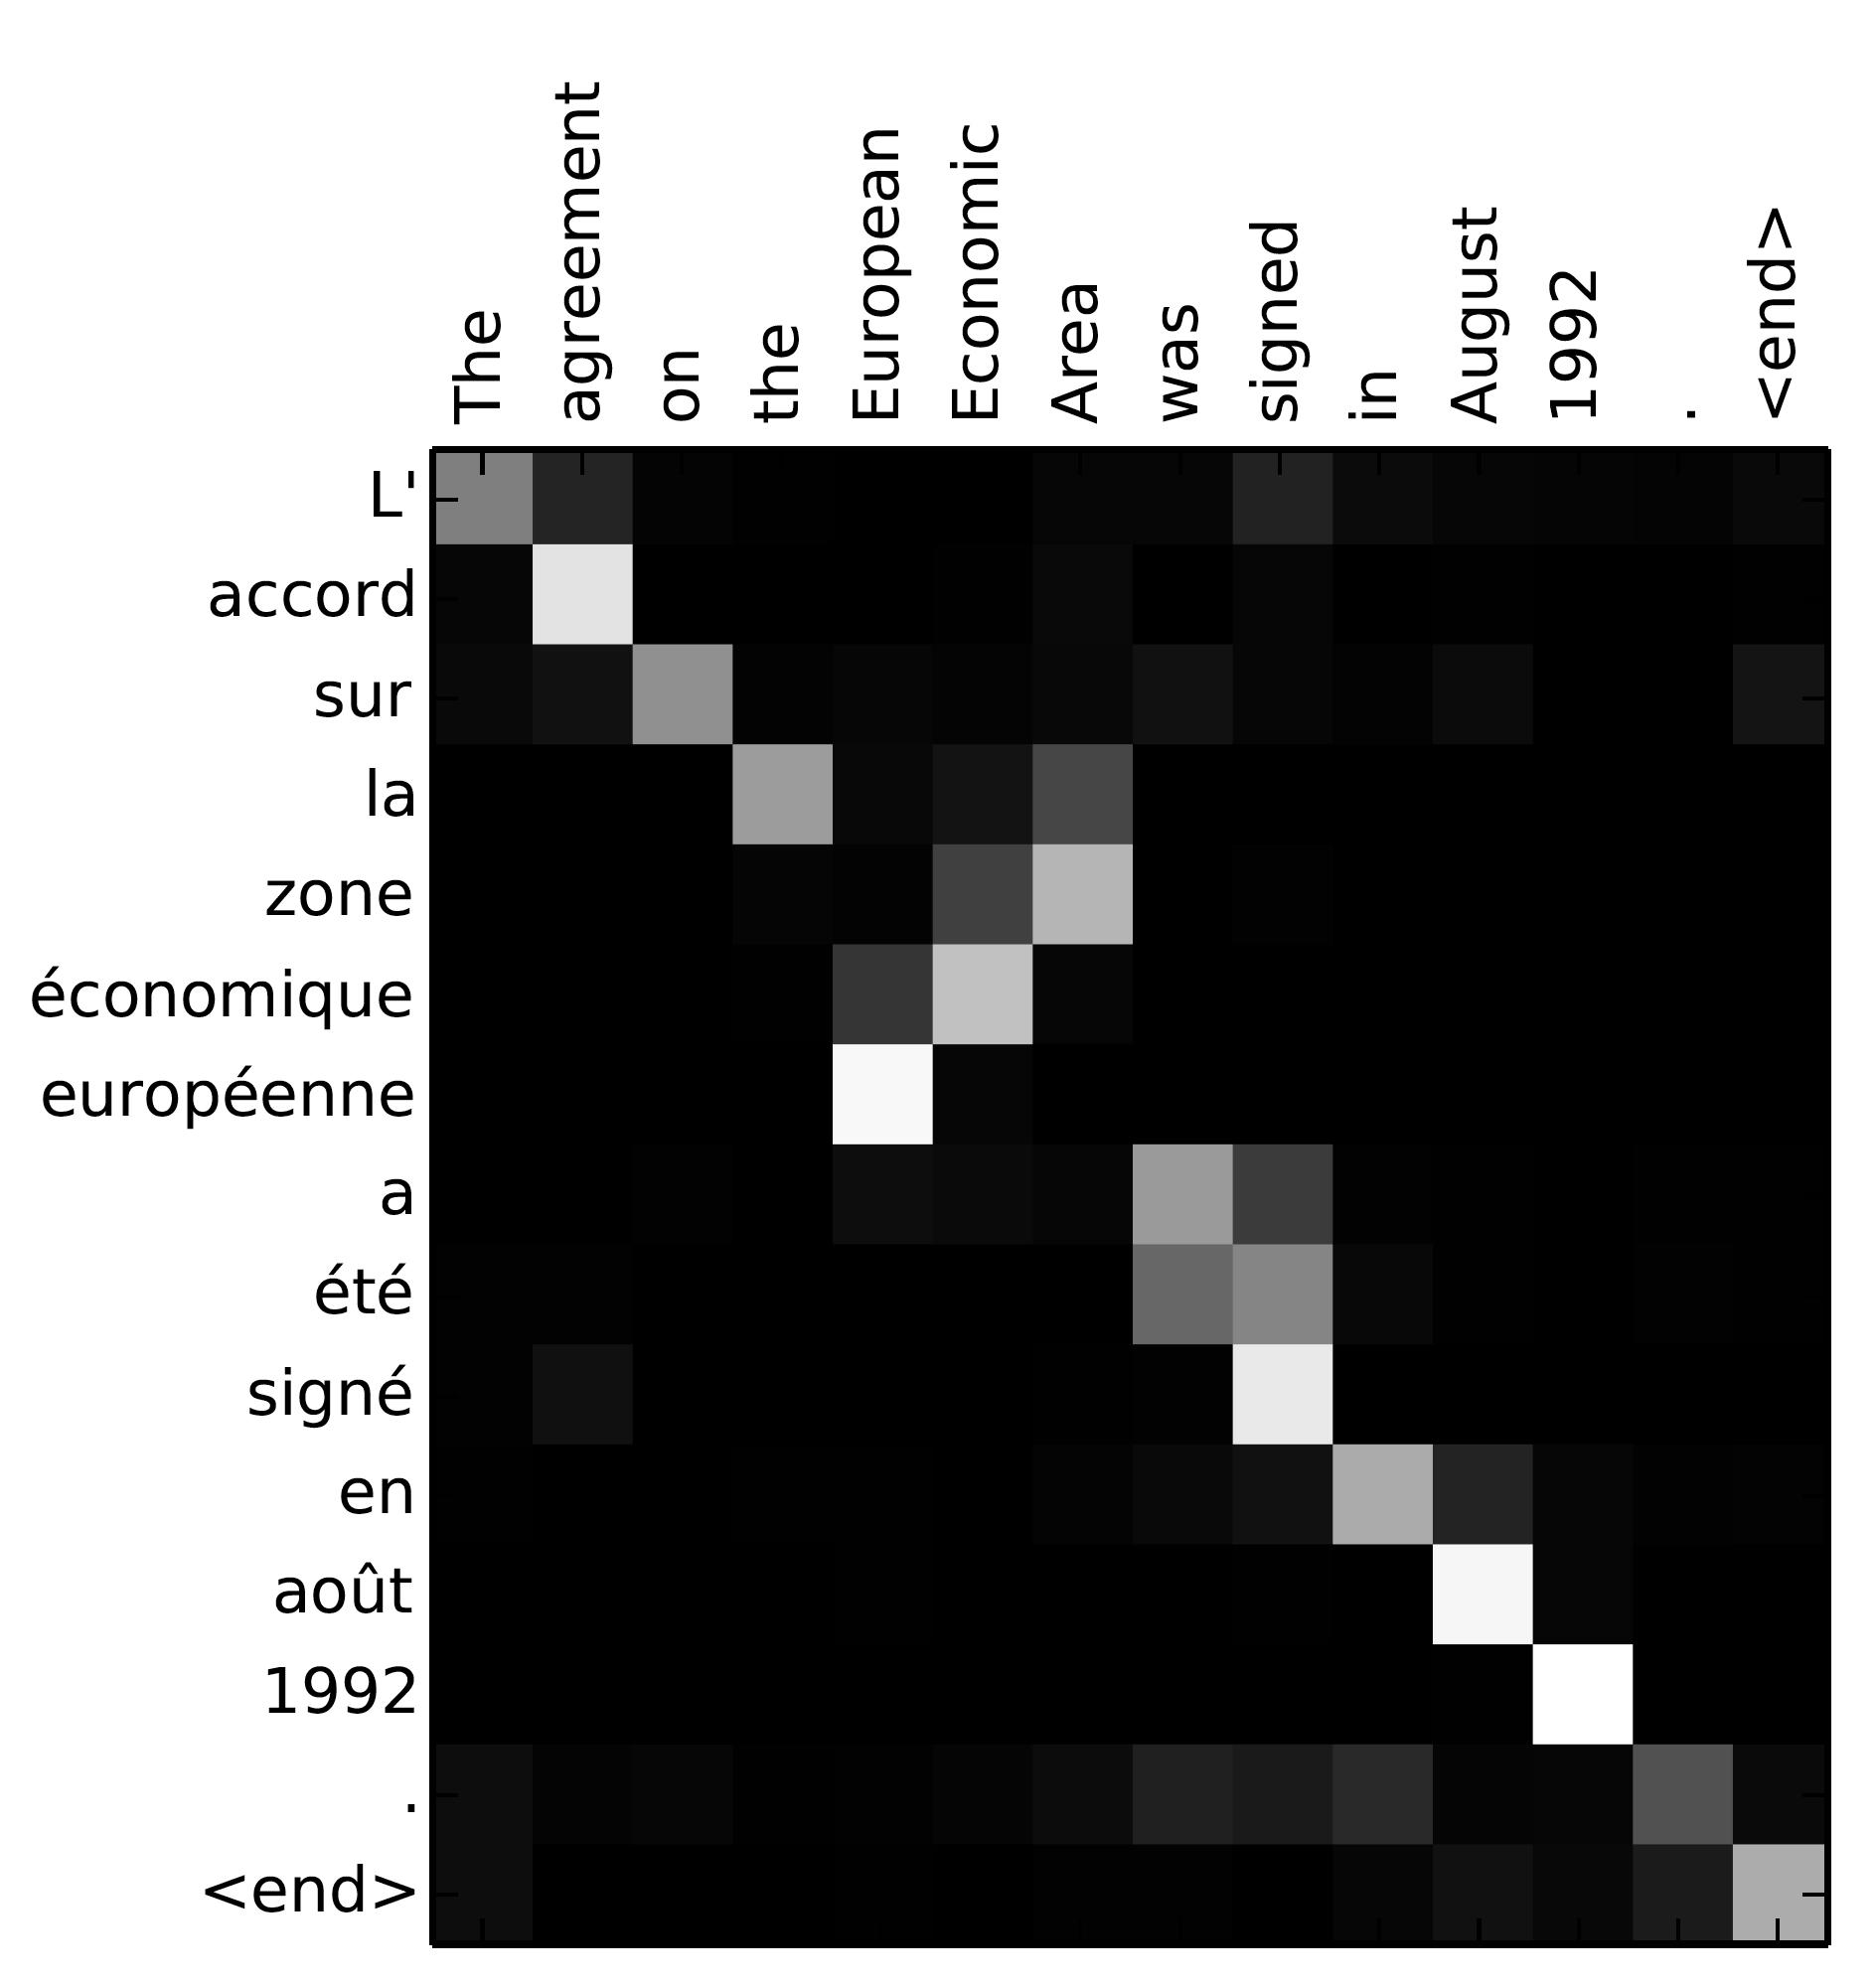
\includegraphics[width=0.6\textwidth]{images/attention_hm.jpg}
    \caption{Heatmap di Attention per task di traduzione.}
    \label{fig:attention-hm}
    \tiny{Fonte: https://github.com/tensorflow/nmt/blob/365e7386e6659526f00fa4ad17eefb13d52e3706/nmt/g3doc/img/attention\_vis.jpg}
\end{figure}

Più precisamente, questa heatmap correla ogni parola in input con ogni parola in output, formando una griglia dove la cella $ij$ si illumina con un colore più luminoso quanto più la parola $j$ in input è legata alla parola $i$ in output. È interessante notare che, in generale, le celle lungo la diagonale principale sono più luminose, rispecchiando la tendenza a mantenere l'ordine delle parole, anche tra lingue differenti. Tuttavia, osservando la sequenza ``European Economic Area'' è evidente come, a causa dell'inversione dell'ordine delle parole in francese (``européenne économique zone''),la correlazione più forte si discosti dalla diagonale principale.

\subsubsection{Funzionamento}
Un modello che fa uso di attention si discosta dai classici modelli Seq2Seq RNN in due modi principalmente. 

In primo luogo, a differenza di quanto succedeva prima, l'encoder passa \emph{tutti} i vettori di stato nascosto al decoder prodotti dalla consumazione progressiva delle parole in input. Cioè lo schema in Figura \ref{fig:seq2seq-rnn} diventa come quello mostrato in Figura \ref{fig:seq2seq-attention}.

\begin{figure}
    \centering
    \begin{tikzpicture}[>=Stealth, node distance=1cm, thick,
    container/.style={draw, rectangle, inner sep=0.2cm, align=center},
    bigbox/.style={draw, rectangle, minimum height=2.5cm, minimum width=10.52cm, align=center},
    box/.style={draw, rectangle, minimum height=2.3cm, minimum width=2.2cm, align=center},
    context/.style={draw, rectangle, minimum height=0.4cm, minimum width=1.6cm, align=center},
    transparent/.style={rectangle, fill=white, align=center}]

    %encoding box
    \node [bigbox, label=above:Encoding Stage] (encoding_stage) {};

    %encoder 1,2,3
    \node [box, xshift=0.1cm, anchor=west] at (encoding_stage.west) (encoder1) {Encoder RNN};
    \node [box, right=0.9cm of encoder1] (encoder2) {Encoder RNN};
    \node [box, right=0.9cm of encoder2] (encoder3) {Encoder RNN};
    
    % Transparent Nodes below Encoders
    \node [transparent, below=1.5cm of encoder1] (sono) {Sono};
    \node [transparent, below=1.5cm of encoder2] (uno) {uno};
    \node [transparent, below=1.5cm of encoder3] (studente) {studente};
    \node [transparent, xshift=2.8cm, anchor=west] at (encoding_stage.east) (decoder) {};

    % Contexts
    \path (encoder1.east) -- (encoder2.west) 
    node [context, rotate=90, midway] (context1) {$\mathbf{h}_1$};
    
    \path (encoder2.east) -- (encoder3.west) 
    node [context, rotate=90, midway] (context2) {$\mathbf{h}_2$};


    \path (encoding_stage.east) -- (decoder)
    node[context, rotate=90, midway] (context2_passed) {$\mathbf{h}_2$};
    
    \node [context, rotate=90, above=0pt of context2_passed, yshift=0.05cm] (context1_passed) {$\mathbf{h}_1$};
    \node [context, rotate=90, above=0pt of context2_passed, yshift=-1.4cm] (context3_passed) {$\mathbf{h}_3$};


    % Arrows
    \draw [->] ([yshift=-0.9cm]encoder1.east) -- ([yshift=-0.9cm]encoder2.west);
    \draw [->] ([yshift=-0.9cm]encoder2.east) -- ([yshift=-0.9cm]encoder3.west);
    \draw [->] (sono) -- (encoder1);
    \draw [->] (uno) -- (encoder2);
    \draw [->] (studente) -- (encoder3);
    \draw [->] ([yshift=-0.9cm]encoding_stage.east) -- ([yshift=-0.9cm]decoder.west);
\end{tikzpicture}
    \caption{Schema di funzionamento della fase di encoding in un modello di attention.}
    \label{fig:seq2seq-attention}
\end{figure}


In secondo luogo, il decoder, impiega una procedura ulteriore, chiamata appunto \emph{attention} a ogni step, operando nel seguente modo per concentrarsi sulla porzione pertinente della frase in input:
\begin{enumerate}
\item Analizza tutti gli hidden state ricevuti dall'encoder. Ognuno di questi hidden state è prevedibilmente più strettamente associato alla parola dell'input che l'encoder ha processato nel corrispondente step; così, come mostrato in Figura \ref{fig:seq2seq-attention}, l'hidden state $\mathbf{h}_2$ è prevalentemente correlato alla seconda parola, $\mathbf{h}_3$ alla terza, e così via. Inoltre, è necessario l'hidden state del decoder nello step corrente.
    \item Assegna ad ogni vettore uno score in relazione allo stato nascosto del decoder all'iterazione $t$ corrente (che chiameremo $\mathbf{s}_t$). Questo score può essere calcolato in diversi modi. Le due modalità seguenti sono le più note:
    \begin{enumerate}
        \item \emph{Additive Attention}. Si calcola con 
        \begin{equation*}
            \text{score}(\mathbf{h}_i) = \mathbf{v}_a^T \tanh{\left(\mathbf{W}_a [ \mathbf{s}_t;\mathbf{h}_i ]\right)}
        \end{equation*}
        dove il ; rappresenta la concatenazione dei vettori e $\mathbf{v}_a, \mathbf{W}_a$ sono dei parametri che il modello apprende in fase di training.
        Fra le due questa risulta essere la più espressiva, cioè è in grado di modellare relazioni più complesse e non lineari tra gli stati nascosti grazie all'uso della funzione di attivazione tanh, tuttavia è estremamente costosa da calcolare.
        \item \emph{Multiplicative Attention}. Si calcola con
        \begin{equation*}
            \text{score}(\mathbf{h}_i) = \mathbf{s}_t^T \mathbf{W}_a \mathbf{h}_i
        \end{equation*}
        Questa formula ha diversi pregi fra cui l'efficienza computazionale (richiede solo operazioni di prodotto scalare e matriciale) e semplice. Tuttavia è intrinsecamente lineare, e questo può limitare la potenzialità di catturare relazioni complesse nei dati.
    \end{enumerate}
    \item Successivamente, si applica la funzione softmax su tutti gli score, che amplifica gli hidden state con score elevati e attenua quelli con score bassi (in pratica, la softmax genera un valore più alto per gli stati con score maggiore e uno più basso per quelli con score minore). 

    \item Ogni vettore è quindi moltiplicato per il rispettivo score (a cui è stata applicata precedentemente la softmax) e i risultati sono sommati, formando così il context vector del decoder per l'iterazione attuale.
\end{enumerate}

In sintesi, se ci troviamo, ad esempio, al quarto step del processo, dopo aver generato i tre vettori di stato nascosto nell'encoder nei primi tre step e averli trasmessi al decoder, la generazione del primo context vector nel decoder (utilizzato, come nei modelli seq2seq RNN, per generare la prima parola in output) avverrà come rappresentato in Figura \ref{fig:attention_scheme}.

\begin{figure}
    \centering
    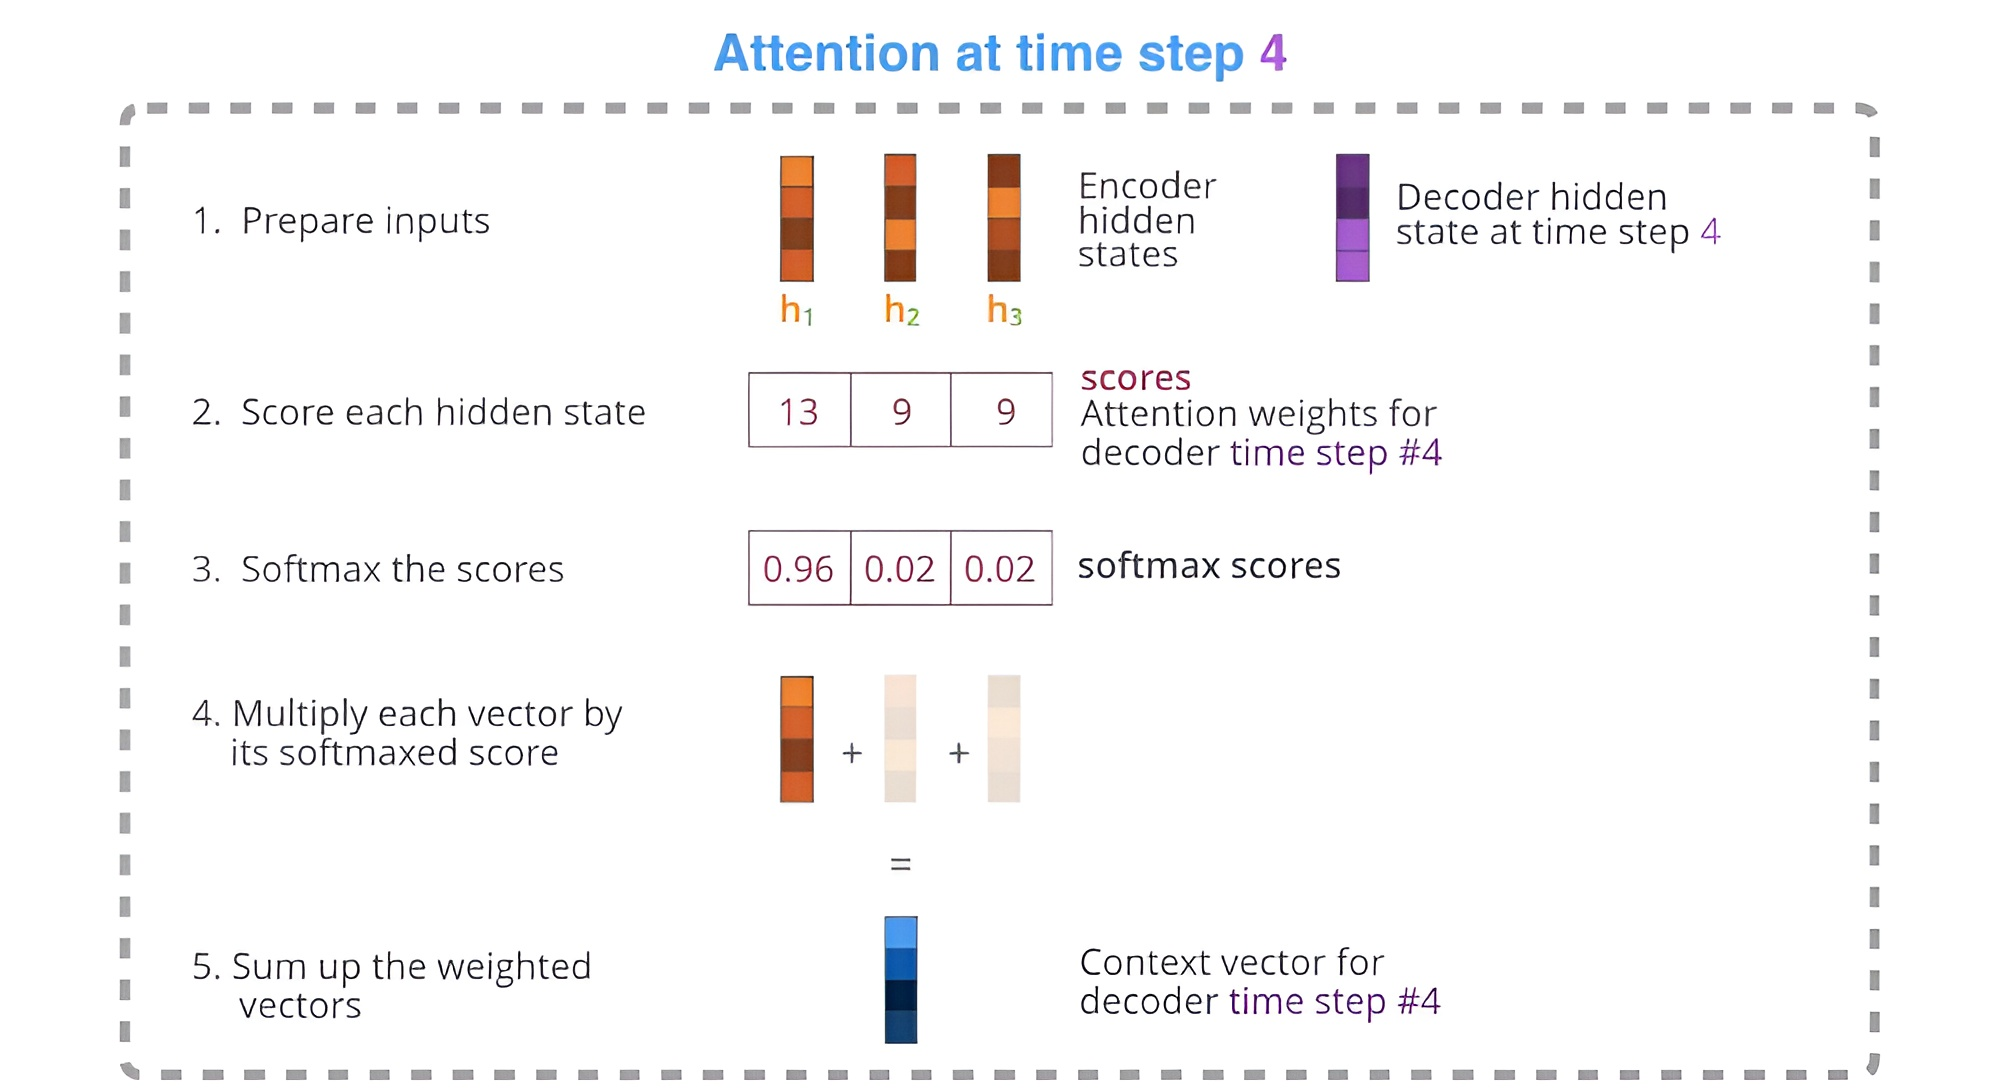
\includegraphics[width=\textwidth]{images/attention_process.jpg}
    \caption{Schema di funzionamento meccanismo di attention.}
    \label{fig:attention_scheme}
    \tiny{https://jalammar.github.io/visualizing-neural-machine-translation-mechanics-of-seq2seq-models-with-attention/}
\end{figure}

Il primo passaggio consiste nella preparazione dei vettori di input, ossia gli hidden state $h1, h2, h3$ ell'encoder e l'hidden state del decoder al quarto passo. Successivamente, si calcolano gli score dei tre hidden state dell'encoder e si applica la softmax su di essi per enfatizzare i valori degli score più alti e ridurre quelli più bassi. Si moltiplica la softmax per ogni hidden state e poi si sommano insieme.
Questo equivale a:
\begin{equation*}
\text{context}_n = \sum_{i=1}^{n-1} \left( \text{Softmax}(\text{score}(\mathbf{h}_i)) \cdot h_i \right)
\end{equation*}
dove il prodotto è da intendersi come prodotto scalare (cioè i termini si moltiplicano uno ad uno e poi si sommano fra loro).

Per sintetizzare il processo eseguito quando si fornisce una stringa, ad esempio ``Sono uno studente'', a un modello Seq2Seq con Attention per un compito di traduzione, i seguenti passaggi vengono eseguiti:

\begin{enumerate}
    \item Al termine della fase di encoding, l'encoder trasmette al decoder i tre hidden state, denotati come ($\mathbf{h}_1, \mathbf{h}_2, \mathbf{h}_3$), generati durante l'elaborazione delle tre parole che compongono la stringa di input.
    \item Nella quarta iterazione (considerando le tre iterazioni precedenti eseguite dall'encoder), il decoder riceve in input l'embedding della stringa speciale di terminazione <END> e uno hidden state iniziale del decoder, denotato come $\mathbf{h}_{\text{init}}$ (si ricorda che anche il decoder è una RNN, pertanto ad ogni iterazione prenderà in input uno stato nascosto e un embedding). 
    \item Attraverso il meccanismo di attention, precedentemente definito, si determina un context vector, $\mathbf{c}_4$, che viene concatenato all'hidden state $\mathbf{h}_4$ prodotto dal decoder RNN a seguito della computazione sull'hidden state iniziale $\mathbf{h}_{\text{init}}$ e la stringa di terminazione <END>. 
    \item La concatenazione $[\mathbf{c}_4 ; \mathbf{h}_4]$ è successivamente inoltrata a una rete neurale feed-forward che genera la parola per il passo corrente. 
\end{enumerate}

Successivamente, la parola generata al passo 4 è utilizzata dal decoder come input per la quinta iterazione. In questo passaggio, il decoder elabora la parola e l'hidden state 4 in input, generando un nuovo hidden state, $\mathbf{h}_5$ che verrà concatenato al vettore di contesto $\mathbf{c}_5$ calcolato come prima. La concatenazione $[\mathbf{c}_5 ; \mathbf{h}_5]$ fiene passato alla FNN che produce la seconda parola di output. 
viene poi fornita alla rete neurale feed-forward che produce la seconda parola in output. Il procedimento si ripete in modo analogo anche per la produzione della terza parola. L'intero processo è illustrato schematicamente nella Figura \ref{fig:attention_dance}.

\begin{figure}
    \centering
    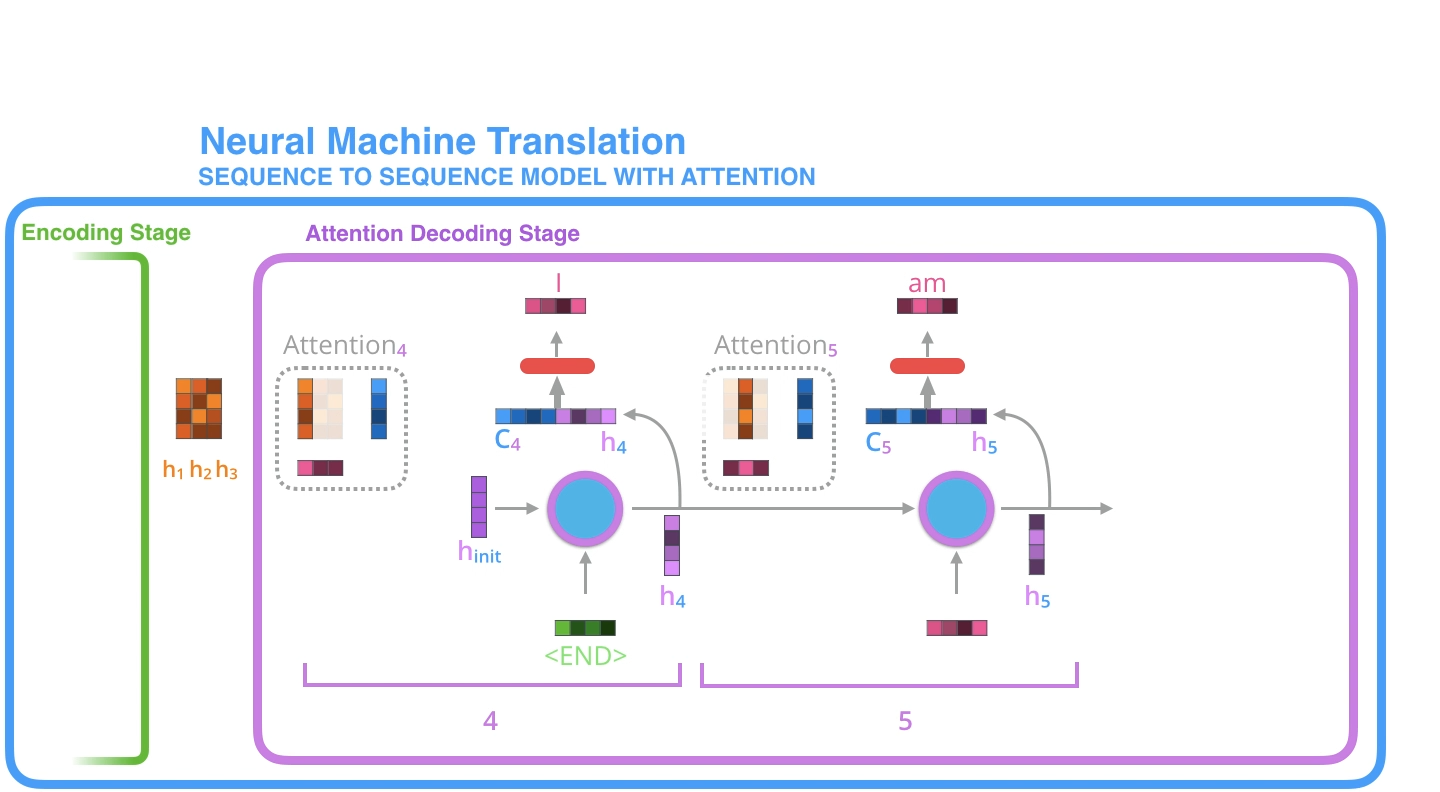
\includegraphics[width=\textwidth]{images/attention_schema.png}
    \caption{Schema di funzionamento di un decoder con attention.}
    \label{fig:attention_dance}
    \tiny{https://jalammar.github.io/visualizing-neural-machine-translation-mechanics-of-seq2seq-models-with-attention/}
\end{figure}


\subsection{Transformers}
Architettura formalmente presentata nel paper intitolato ``Attention is All You Need'' \cite{DBLP:journals/corr/VaswaniSPUJGKP17}, con l'obiettivo di superare i modelli sequence-to-sequence basati su RNN e meccanismi di Attention, dettagliati nei paragrafi precedenti. 

Il titolo del paper suggerisce la novità cardine introdotta dagli autori: una nuova architettura, denominata \emph{transformers}, che si fonda esclusivamente sul principio dell'attention, eliminando la necessità di impiegare reti neurali ricorrenti. Questo approccio ha dimostrato non solo la sua validità, ma ha anche permesso di raggiungere un significativo miglioramento delle performance nei compiti di elaborazione del linguaggio naturale.

\subsubsection{Funzionamento} L'architettura basata su Transformers, come sarà illustrato, mantiene una struttura non dissimile da quella dei modelli sequence-to-sequence (seq2seq) implementati con Reti Neurali Ricorrenti (RNN). Specificatamente, i modelli seq2seq sono delineati da una struttura encoder-decoder. In tale configurazione, l'encoder è responsabile per trasformare una sequenza di rappresentazioni simboliche (i.e. parole) 
\begin{equation*}
(x_1, \dots, x_n)
\end{equation*}
in una corrispondente sequenza di rappresentazioni continue (gli stati nascosti),
\begin{equation*}
\mathbf{H} = (\mathbf{h}_1, \mathbf{h}_2, \dots, \mathbf{h}_n)
\end{equation*}
Una volta ottenuto $\mathbf{H}$, il decoder genera sequenzialmente una serie di simboli (parole)
\begin{equation*}
(y_1,y_2, \dots, y_m)
\end{equation*}
un elemento alla volta. Ad ogni passo, il modello, essendo auto-regressivo, impiega i simboli precedentemente generati come input aggiuntivo per la produzione del simbolo successivo, consumando, quindi, i simboli prodotti in combinazione con lo stato nascosto precedente per generare la sequenza di output.

I Transformers sono strutturati seguendo un principio analogo, caratterizzati da $N=6$ layer di \emph{encoder} concatenati e altrettanti layer di \emph{decoder}, disposti in maniera analoga.

Quello che cambia è il contenuto di decoder ed encoder. Come mostra figura \ref{fig:transformer-base}, avremo 
\begin{itemize}
    \item L'input dell'\emph{encoder} attraversa in quest'ordine un layer di \emph{self attention} (definita nel dettaglio in seguito), che consente all'encoder di capire come codificare la parola osservando la relazione che questa ha con le altre e una rete feed forward (FNN).
    \item Il \emph{decoder} è fatto in maniera analoga, avendo in più fra la FNN e il layer di self attention, un layer di attention come è stata definita nel capitolo precedente, che gli consente di concentrarsi sulle parti rilevanti della sequenza di input per produrre l'output. 
\end{itemize}



\begin{figure}
    \centering
    \begin{tikzpicture}[>=Stealth, node distance=1cm, thick,
            encoder/.style={draw, rectangle, minimum height=2.5cm, minimum width=5.5cm, align=center},
            decoder/.style={draw, rectangle, minimum height=3.77cm, minimum width=5.5cm, align=center},
            box/.style={draw, rectangle, minimum height=1cm, minimum width=5.3cm, align=center},
            transparent/.style={rectangle, fill=white, align=center}]
% encoder
\node [encoder] (encoder) {};
\node [above=1mm of encoder.north, xshift=-1.7cm] {Encoder};
\node [box, below=0.1cm of encoder.north] (fnn) {Feed Forward};
\node [box, above=0.1cm of encoder.south] (sal) {MultiHead Self-Attention};
\node [transparent, above=0.3cm of encoder.north] (up_encoder_arrow) {};
\node [transparent, below=0.3cm of encoder.south] (low_encoder_arrow) {};


%decoder
\node [decoder, right=7cm of encoder.west] (decoder) {};
\node [above=1mm of decoder.north, xshift=-1.7cm] {Decoder};
\node [box, below=0.1cm of decoder.north] (fnn_decoder) {Feed Forward};
\node [box] (eda) at (decoder) {Encoder-Decoder Attention};
\node [box, above=0.1cm of decoder.south] (sal_decoder) {Masked MH Self-Attention};
\node [transparent, above=0.3cm of decoder.north] (up_decoder_arrow) {};
\node [transparent, below=0.3cm of decoder.south] (low_decoder_arrow) {};


% Arrow
\draw [->] (sal) -- (fnn);
\draw [->] (low_encoder_arrow) -- (sal);
\draw [->] (fnn) -- (up_encoder_arrow);

\draw [->] (sal_decoder) -- (eda);
\draw [->] (eda) -- (fnn_decoder);
\draw [->] (low_decoder_arrow) -- (sal_decoder);
\draw [->] (fnn_decoder) -- (up_decoder_arrow);

\draw [->] (encoder) -- (decoder);

\end{tikzpicture}

    \caption{Architettura di base di un Transformers}
    \label{fig:transformer-base}
\end{figure}

\paragraph{Self-Attention}

La \emph{self-attention} opera, a livello concettuale, in maniera analoga alla meccanica dell'attention delineata nel precedente paragrafo, permettendo al modello di discernere le relazioni semantiche intrinseche fra le parole presenti nella sequenza di input. Ciò che distingue la \emph{self-attention} è la metodologia attraverso cui vengono calcolati gli score, utilizzati successivamente per generare i vettori di contesto.

Considerando la frase:
\begin{center}
    ``The animal didn't cross the street because it was too tired''
\end{center}
la \emph{self-attention} consente al modello di associare correttamente il pronome ``it'' con ``animal'' piuttosto che con ``street''. Questa correlazione è illustrata graficamente in Figura \ref{fig:attention-rel}, dove l'intensità cromatica di una parola denota il grado di correlazione con la parola ``it''.

\begin{figure}
    \centering
    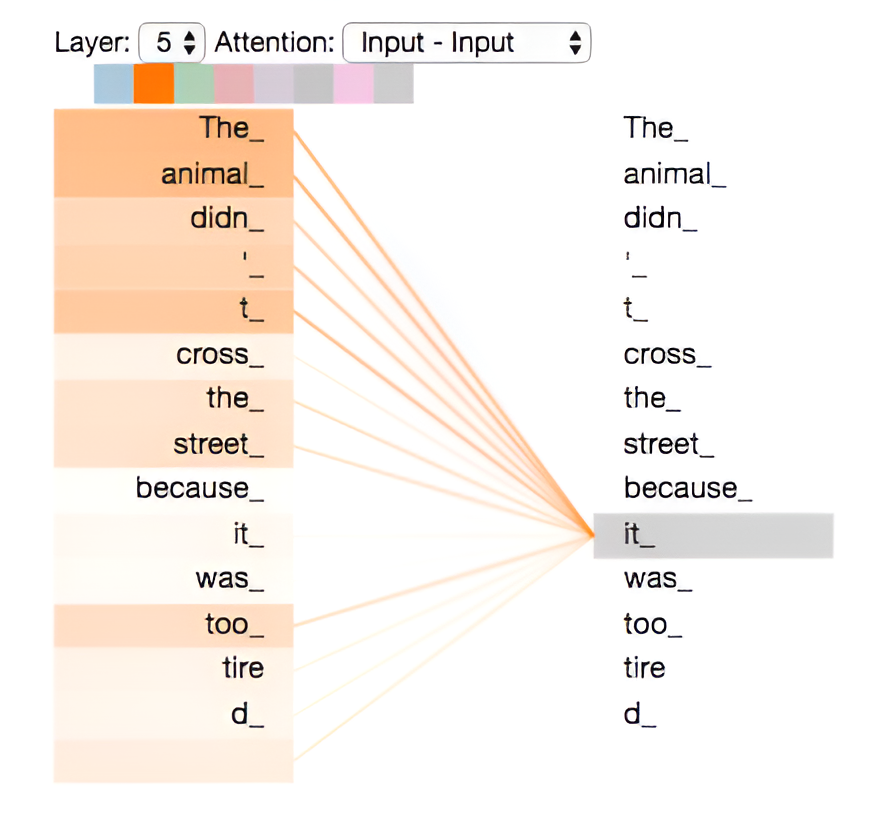
\includegraphics[width=0.6\textwidth]{images/transformer_self-attention_visualization.png}
    \caption{Visualizzazione grafica della self attention per una frase.}
    \label{fig:attention-rel}
\end{figure}

Il procedimento operativo della \emph{self-attention} può essere suddiviso nei seguenti passi:
\begin{enumerate}
    \item Inizialmente, da una matrice di embeddings di input, denotata come $\mathbf{X}$, (una riga per ogni embedding), vengono generate tre matrici distinte: matrice delle \emph{query} $\mathbf{Q}$ ,matrice delle \emph{chiavi} $\mathbf{K}$ e matrice dei valori $\mathbf{V}$. Ogni riga delle suddette matrici corrisponde a un embedding distinto, calcolato mediante la moltiplicazione della matrice $\mathbf{X}$ per delle matrici di pesi $\mathbf{W^Q},\mathbf{W^K},\mathbf{W^V}$ apprese durante la fase di addestramento, come illustrato in Figura \ref{fig:qkv-prod}.
    \item Successivamente, vengono calcolati gli score di correlazione per ogni parola nella sequenza di input, con ciascuna delle altre parole presenti, generando $n^2$ score, ove $n$ rappresenta il numero di parole nella sequenza. Gli score di attention sono ottenuti attraverso i seguenti passaggi:
    \begin{itemize}
        \item Ogni riga di $\mathbf{Q}$ viene moltiplicata per ogni riga di $\mathbf{K}$ (nel concreto $\mathbf{K}$ verrà trasposta per consentire questo prodotto).
        \item Il risultato ottenuto viene normalizzato dividendo per un \emph{fattore di scala} $\sqrt{d_k}$ che non è altro che la dimensione della matrice delle chiavi. Questo serve perché la dimensione delle chiavi (e anche di query) sarà proporzionale al numero di elementi in input perciò la moltiplicazione di ogni query per ogni chiave potrebbe portare a valori molto grandi se l'input è esteso. Questo passaggio è fatto al fine di mitigare l'incremento dei valori derivante da sequenze di input ampie. 
        \item Si procede applicando la funzione softmax a ciascuno degli score ottenuti. Tale operazione ha lo scopo di quantificare il grado di rilevanza della parola $i$-esima in posizione $j$. È naturale aspettarsi che, quando $i = j$ lo score risultante tenda ad essere più elevato. L'obiettivo di questa procedura è preservare l'integrità delle parole di interesse, mentre si attenua l'importanza di quelle considerate irrilevanti per la generazione del segmento di output desiderato.
        \item Infine, ciascun elemento ottenuto viene moltiplicato per ogni elemento della matrice dei valori $\mathbf{V}$. Questo produce una matrice di attention $\text{Attention}(\mathbf{Q,K,V})$ contenente i valori di self attention di ogni parola di input.
    \end{itemize}
    L'uso di matrici in questo contesto facilita il calcolo parallelo degli score, permettendo di processare l'intera sequenza di input in un unico passaggio computazionale.
    \begin{equation}
    \label{eq:attention}
        \text{Attention}(\mathbf{Q,K,V}) = \text{Softmax}\left( \frac{\mathbf{Q}\mathbf{K}^T}{\sqrt{d_k}} \right) \mathbf{V}
    \end{equation}

    Graficamente questa procedura, chiamata nel paper \emph{scaled dot product attention}, si riassume nello schema in figura \ref{fig:dotproduct-attention} (lo step di mascheratura opzionale verrà chiarito in seguito).
    \begin{figure}
        \centering
        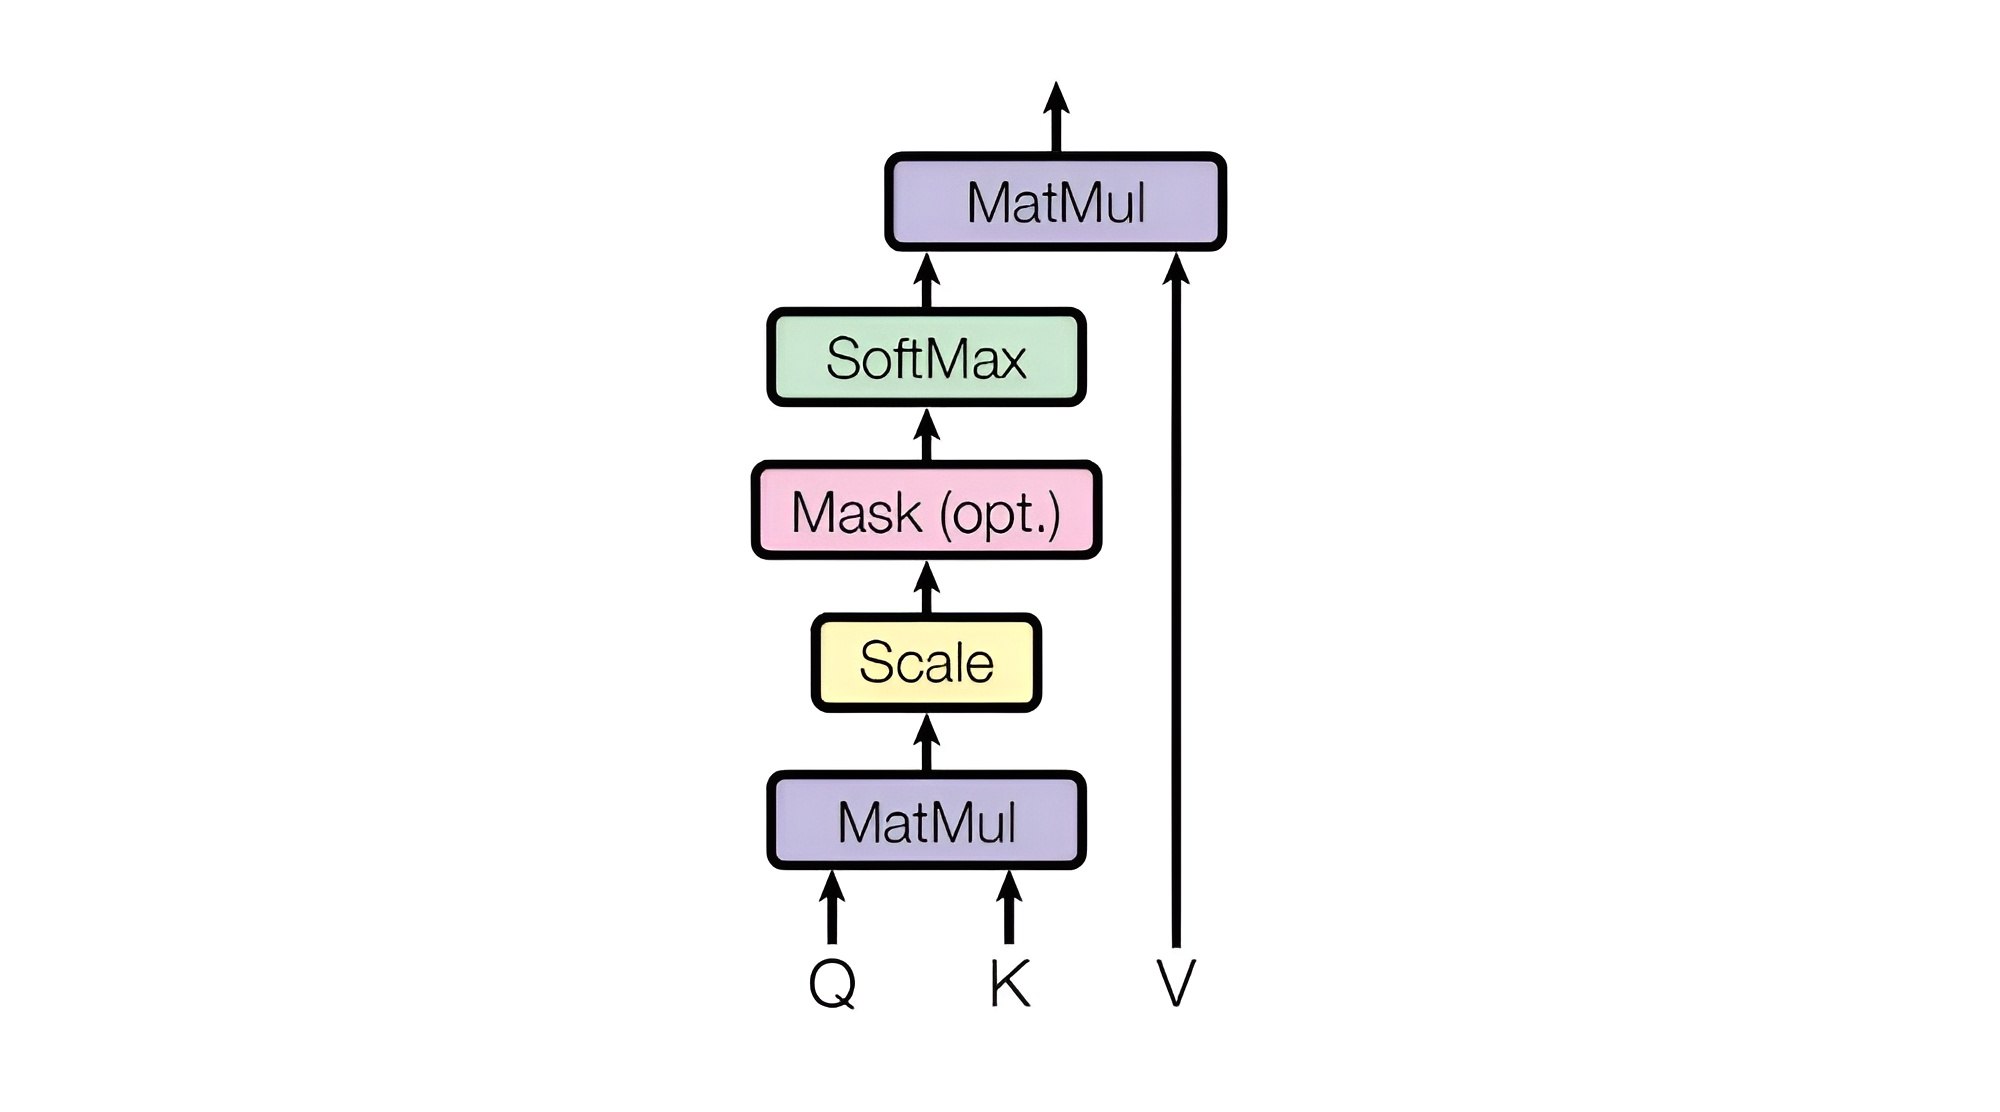
\includegraphics[width=0.8\textwidth]{images/attention_product.png}
        \caption{Scaled dot product attention schema.}
        \label{fig:dotproduct-attention}
    \end{figure}
    
\end{enumerate}


\begin{figure}
    \centering
    \begin{tikzpicture}[>=Stealth,
        vector element/.style={draw, rectangle, minimum width=0.6cm, minimum height=0.6cm, align=center}
    ]
        %query
        
        \matrix[row sep=0pt,column sep=0pt] (x1) {
            \node [vector element] (x00) {}; & \node [vector element] (x01) {}; & \node [vector element] (x02) {}; & \node [vector element] (x03) {}; \\
            \node [vector element] (x10) {}; & \node [vector element] (x11) {}; & \node [vector element] (x12) {}; & \node [vector element] (x13) {}; \\
        };
        \node [above=0.1cm of x1] {$\mathbf{X}$};

        \node [right=0.4cm of x1] (times_x1) {$\times$};

        \matrix[row sep=0pt,column sep=0pt, right=0.4cm of times_x1] (wq) {
            \node [vector element] (x00) {}; & \node [vector element] (x01) {}; & \node [vector element] (x02) {}; \\
            \node [vector element] (x10) {}; & \node [vector element] (x11) {}; & \node [vector element] (x12) {}; \\
            \node [vector element] (x20) {}; & \node [vector element] (x21) {}; & \node [vector element] (x22) {}; \\
            \node [vector element] (x30) {}; & \node [vector element] (x31) {}; & \node [vector element] (x32) {}; \\
        };
        \node [above=0.1cm of wq] {$\mathbf{W^Q}$};

        \node [right=0.4cm of wq] (equals_x1) {$=$};

        \matrix[row sep=0pt,column sep=0pt, right=0.4cm of equals_x1] (q) {
            \node [vector element] (x00) {}; & \node [vector element] (x01) {}; & \node [vector element] (x02) {}; \\
            \node [vector element] (x10) {}; & \node [vector element] (x11) {}; & \node [vector element] (x12) {}; \\
        };
        \node [above=0.1cm of q] {$\mathbf{Q}$};


        %key

        \matrix[row sep=0pt,column sep=0pt, below=2cm of x1] (x2) {
            \node [vector element] (x00) {}; & \node [vector element] (x01) {}; & \node [vector element] (x02) {}; & \node [vector element] (x03) {}; \\
            \node [vector element] (x10) {}; & \node [vector element] (x11) {}; & \node [vector element] (x12) {}; & \node [vector element] (x13) {}; \\
        };
        \node [above=0.1cm of x2] {$\mathbf{X}$};

        \node [right=0.4cm of x2] (times_x2) {$\times$};

        \matrix[row sep=0pt,column sep=0pt, right=0.4cm of times_x2] (wk) {
            \node [vector element] (x00) {}; & \node [vector element] (x01) {}; & \node [vector element] (x02) {}; \\
            \node [vector element] (x10) {}; & \node [vector element] (x11) {}; & \node [vector element] (x12) {}; \\
            \node [vector element] (x20) {}; & \node [vector element] (x21) {}; & \node [vector element] (x22) {}; \\
            \node [vector element] (x30) {}; & \node [vector element] (x31) {}; & \node [vector element] (x32) {}; \\
        };
        \node [above=0.1cm of wk] {$\mathbf{W^K}$};

        \node [right=0.4cm of wk] (equals_x2) {$=$};

        \matrix[row sep=0pt,column sep=0pt, right=0.4cm of equals_x2] (k) {
            \node [vector element] (x00) {}; & \node [vector element] (x01) {}; & \node [vector element] (x02) {}; \\
            \node [vector element] (x10) {}; & \node [vector element] (x11) {}; & \node [vector element] (x12) {}; \\
        };
        \node [above=0.1cm of k] {$\mathbf{K}$};

        %value

        \matrix[row sep=0pt,column sep=0pt, below=2cm of x2] (x3) {
            \node [vector element] (x00) {}; & \node [vector element] (x01) {}; & \node [vector element] (x02) {}; & \node [vector element] (x03) {}; \\
            \node [vector element] (x10) {}; & \node [vector element] (x11) {}; & \node [vector element] (x12) {}; & \node [vector element] (x13) {}; \\
        };
        \node [above=0.1cm of x3] {$\mathbf{X}$};

        \node [right=0.4cm of x3] (times_x3) {$\times$};

        \matrix[row sep=0pt,column sep=0pt, right=0.4cm of times_x3] (wv) {
            \node [vector element] (x00) {}; & \node [vector element] (x01) {}; & \node [vector element] (x02) {}; \\
            \node [vector element] (x10) {}; & \node [vector element] (x11) {}; & \node [vector element] (x12) {}; \\
            \node [vector element] (x20) {}; & \node [vector element] (x21) {}; & \node [vector element] (x22) {}; \\
            \node [vector element] (x30) {}; & \node [vector element] (x31) {}; & \node [vector element] (x32) {}; \\
        };
        \node [above=0.1cm of wv] {$\mathbf{W^V}$};

        \node [right=0.4cm of wv] (equals_x3) {$=$};

        \matrix[row sep=0pt,column sep=0pt, right=0.4cm of equals_x3] (v) {
            \node [vector element] (x00) {}; & \node [vector element] (x01) {}; & \node [vector element] (x02) {}; \\
            \node [vector element] (x10) {}; & \node [vector element] (x11) {}; & \node [vector element] (x12) {}; \\
        };
        \node [above=0.1cm of v] {$\mathbf{V}$};
        
        
    \end{tikzpicture}
    \caption{Prodotto matriciale per determinazione delle matrici query, key, value.}
    \label{fig:qkv-prod}
\end{figure}



\paragraph{MultiHead self-attention}
Il processo di attention viene ulteriormente raffinato introducendo un'architettura \emph{MultiHead}. Questo significa che la stessa sequenza di input viene processata \emph{parallelamente} da più layer, chiamati \emph{head}, di attention.
Questo avviene proiettando linearmente le matrici di query $\mathbf{Q}$, chiavi $\mathbf{K}$ e valori $\mathbf{V}$ calcolate in precedenza in $h$ (nel paper originale $h=8$) spazi diversi, moltiplicandole per le seguenti matrici di pesi 
\begin{equation*}
    \mathbf{W}_i^\mathbf{^Q}, \mathbf{W^K}_i, \mathbf{W^V}_i \quad \forall i \in [0, h-1] 
\end{equation*}
apprese in fase di addestramento. 
Una volta ottenute queste matrici proiettate negli $h$ nuovi spazi è possibile calcolare l'attention per ogni head in maniera analoga a quella mostrata nell'equazione \ref{eq:attention}, sostituendo però opportunamente le matrici. Indichiamo con $\text{head}_i$ la matrice risultante dal calcolo dell'attention sull'head $i$-esima.  

\begin{equation*}
    \text{head}_i = \text{Attention}(\mathbf{Q} \mathbf{W}_i^\mathbf{^Q}, \mathbf{K} \mathbf{W}_i^\mathbf{^K}, \mathbf{V} \mathbf{W}_i^\mathbf{^V})
\end{equation*}

Poiché la rete feedforward posta a valle di ogni enconder si aspetta una sola matrice, occorre trovare un modo di passare loro tutti gli $h$ head prodotti. 
Pertanto l'ultimo passaggio che resta da fare è concatenare gli $h$ head e farne il prodotto scalare per una matrice di pesi $\mathbf{W}^O$, anch'essa appresa in fase di addestramento. Questo si traduce nella seguente equazione
\begin{equation*}
    \text{MultiHead}(\mathbf{Q,K,V}) = \text{Concat}(\text{head}_1, \text{head}_2, \dots, \text{head}_h)\mathbf{W}^O
\end{equation*}

Lo schema in Figura \ref{fig:multihead-attention} mostra quanto appena descritto a parole. Le tre matrici originali vengono proiettate in $h$ spazi vettoriali tramite delle trasformazioni lineari (prodotto per matrici di pesi), parallelamente su ciascuna di esse viene calcolata una matrice di self attention. Queste matrici vengono concatenate e poi trasformate linearmente mediante il prodotto scalare per una matrice di pesi. 

\begin{figure}
    \centering
    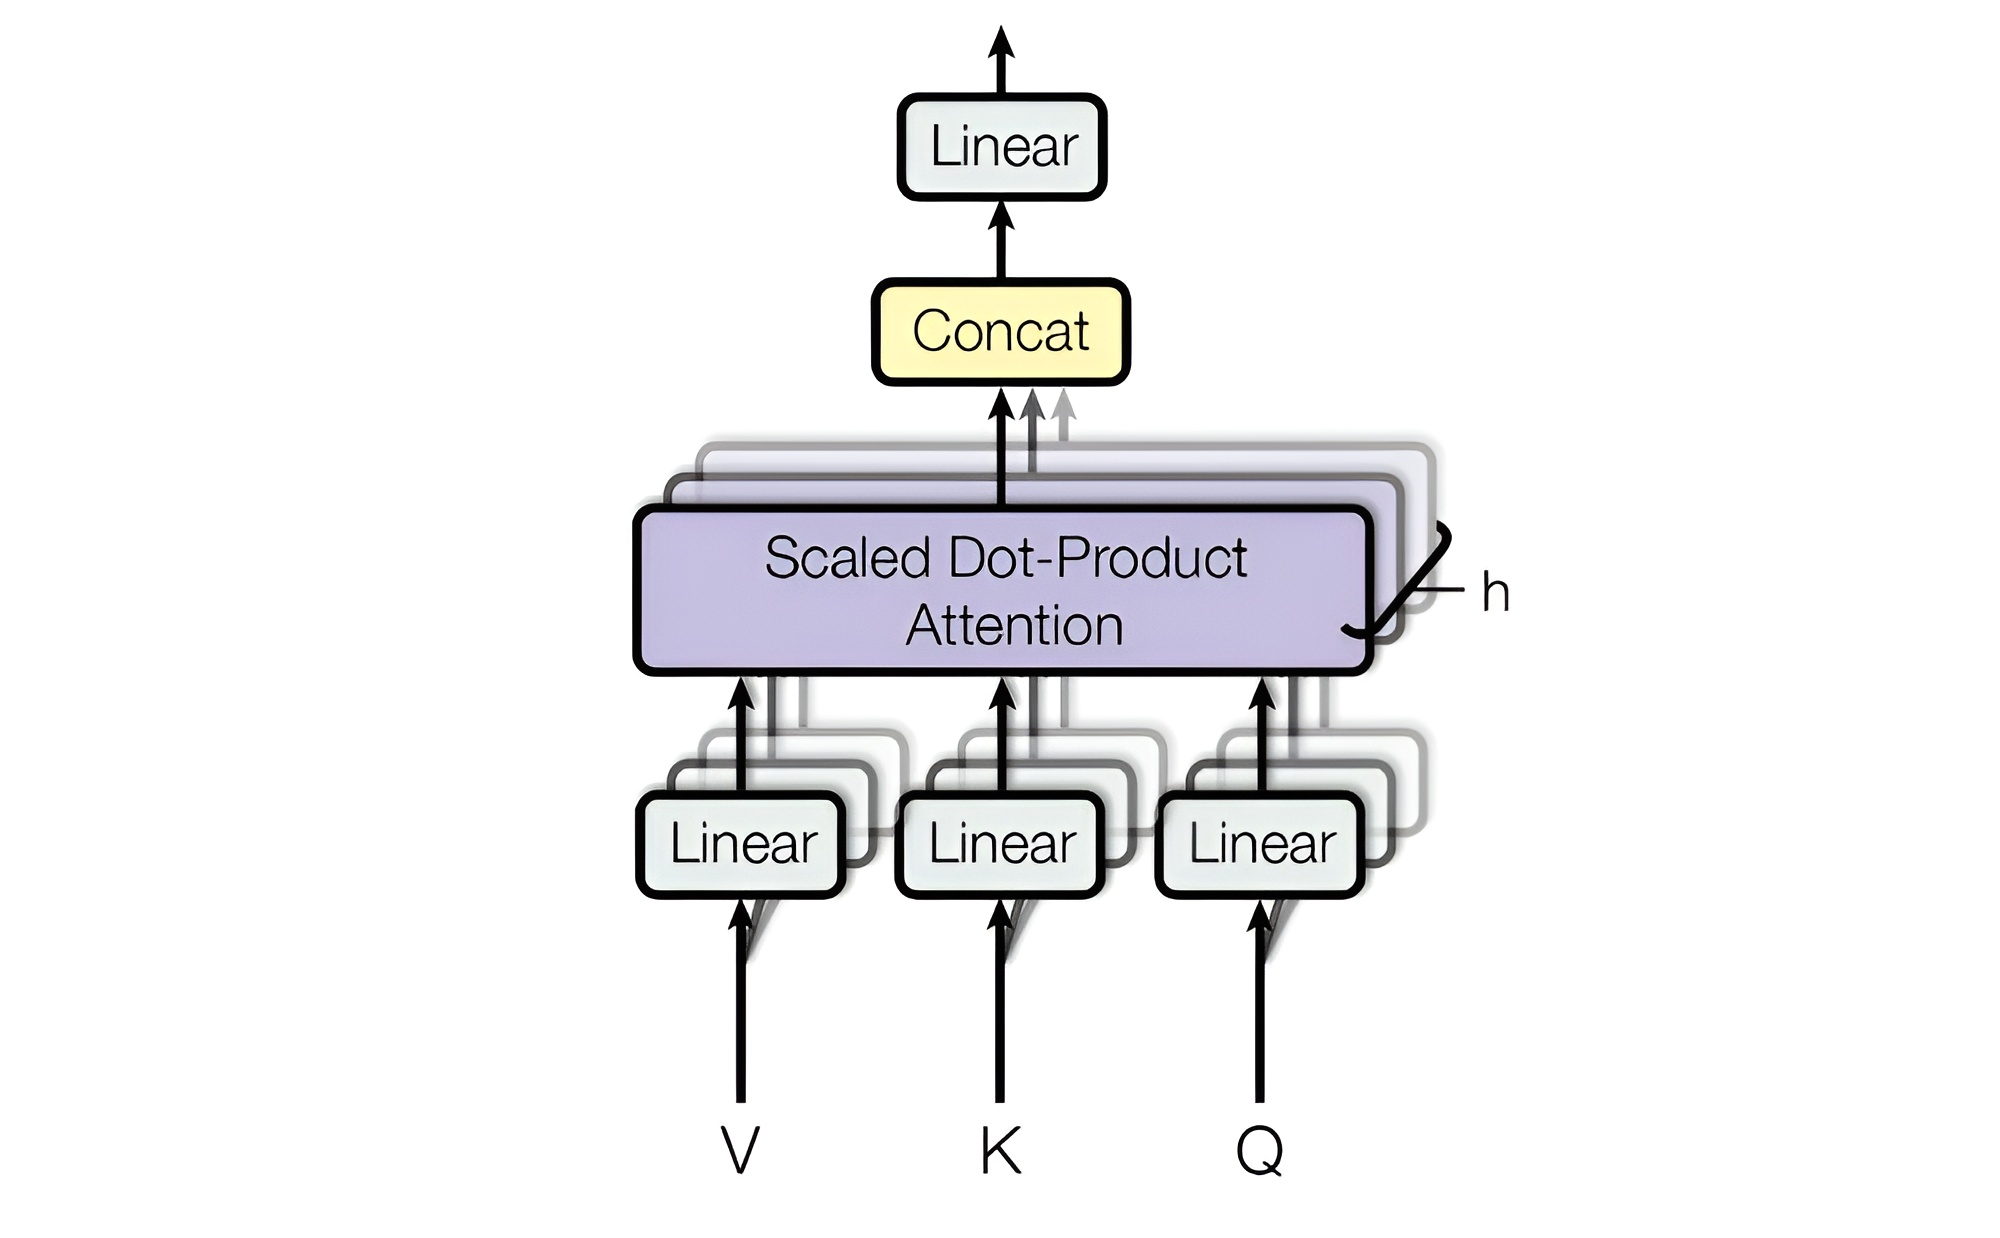
\includegraphics[width=0.8\textwidth]{images/mh_attention.png}
    \caption{MultiHead Attention schema.}
    \label{fig:multihead-attention}
\end{figure}

L'implementazione della MultiHead Self-Attention incrementa la capacità del modello di focalizzarsi su differenti posizioni all'interno del testo in input. Una singola matrice di attention, infatti, incorpora elementi di ogni altra parola presente, ma la predominanza potrebbe essere attribuita all'effettiva parola su cui l'attention è calcolata. Utilizzando più head si riesce ad avere una rappresentazione più globale delle relazioni che intercorrono fra ciascuna parola di input con ciascuna altra.

\paragraph{Positional Encoding}
Poiché l'architettura a transformers non fa uso di ricorrenza (ovvero non è basata su RNN), gli autori del paper \cite{DBLP:journals/corr/VaswaniSPUJGKP17} hanno anche introdotto alla base dello stack di encoders/decoders, un cosiddetto ``\emph{positional encoding}'' per permettere al modello di comprendere la posizione relativa o assoluta delle parole all'interno delle sequenze in input.
Questo encoding può essere fatto in diversi modi, tuttavia quello scelto dagli autori è il seguente

\begin{align*}
    PE_{(pos, 2i)} &= \sin \left( \frac{pos}{10000^{\frac{2i}{d_{\text{model}}}}} \right) \\
    PE_{(pos, 2i+1)} &= \cos \left( \frac{pos}{10000^{\frac{2i}{d_{\text{model}}}}} \right)
\end{align*}

dove 
\begin{itemize}
    \item $pos$ rappresenta la posizione di un determinato token all'interno della sequenza in input.
    \item $i$ varia da 0 a $d_{\text{model}}$ che rappresenta la dimensione degli embeddings. 
\end{itemize}

Queste funzioni hanno la proprietà di permettere al modello di apprendere facilmente a prestare attenzione alle posizioni relative dei token, indipendentemente dalla lunghezza della sequenza.

Questi positional encoding vengono integrati all'interno della matrice degli embeddings semplicemente sommando elemento per elemento la matrice degli embeddings e i corrispettivi encoding posizionali. 

\paragraph{LayerNorm} A seguito di ogni layer dei transformer (i.e. Multi-Head Attention, FNN, ecc.) viene applicata un'operazione di normalizzazione, come descritto in \cite{ba2016layer}. L'obiettivo principale di questa operazione è stabilizzare e accelerare l'addestramento delle reti neurali profonde, facilitando la loro convergenza. L'operazione di normalizzazione può essere rappresentata come:
\begin{equation*}
    \text{LayerNorm}(\mathbf{X} + \mathbf{Z})
\end{equation*}
dove:
\begin{itemize}
    \item $\mathbf{X}$ rappresenta la matrice degli embeddings (a cui sono stati precedentemente sommati i positional encoding).
    \item $\mathbf{Z}$ indica la matrice di output prodotta dal layer precedente all'operazione di normalizzazione.
\end{itemize}

\paragraph{Funzionamento del decoder}
Tutta la tecnologia alla base della componente del decoder è già stata ampiamente trattata ai paragrafi precedenti. 
Come mostra Figura \ref{fig:transformer-base}, il decoder si distingue dall'encoder principalmente per due aspetti:
\begin{enumerate}
    \item Oltre al layer di self-attention e al layer feedforward presenti nell'encoder, il decoder introduce un layer di multihead attention tra questi due. Questo layer consente al decoder di focalizzarsi sull'output dell'encoder, essenziale per operazioni come la traduzione, dove il decoder deve fare riferimento all'input originale (nel contesto di una lingua di partenza) per generare un output appropriato (in una lingua di destinazione).
    
    \item Il layer di self-attention nel decoder è \emph{mascherato} per preservare la sua natura \emph{auto-regressiva}. Questo garantisce che ogni predizione dipenda solo da posizioni precedenti, evitando l'attenzione verso posizioni future. Ciò è realizzato mascherando (impostando a $-\infty$) determinate connessioni, prima di applicare la softmax per quelle che corrispondono a connessioni ``illegali'' (ossia, connessioni a posizioni future), come illustrato in Figura \ref{fig:dotproduct-attention} (Mask opt.). Dopo aver applicato la softmax a valori molto negativi, infatti, questi diventano essenzialmente zero, impedendo di fatto l'attenzione verso le posizioni future.
\end{enumerate}



\paragraph{Linear e Softmax Layers}
Dopo che l'output di tutti i decoder è stato elaborato, abbiamo una serie di vettori numerici. Per convertire questi vettori in parole, vengono applicati i layer \emph{Linear} e \emph{Softmax}. 
\begin{itemize}
    \item Il layer \emph{Linear} è una rete feedforward che proietta i vettori output dallo stack di encoder in uno spazio vettoriale più grande, corrispondente, ad esempio, a un dizionario di 10.000 parole apprese in fase di training. Il vettore in questione è chiamato \emph{vettore di logits}.
    \item Il layer \emph{Softmax} converte gli score prodotti dal layer Linear in probabilità, selezionando l'output basato sulla cella con la probabilità più alta.
\end{itemize}

In conclusione l'architettura a Transformers complessiva e ad alto livello è rappresentata graficamente in figura \ref{fig:transformer}.

\begin{figure} 
    \centering
    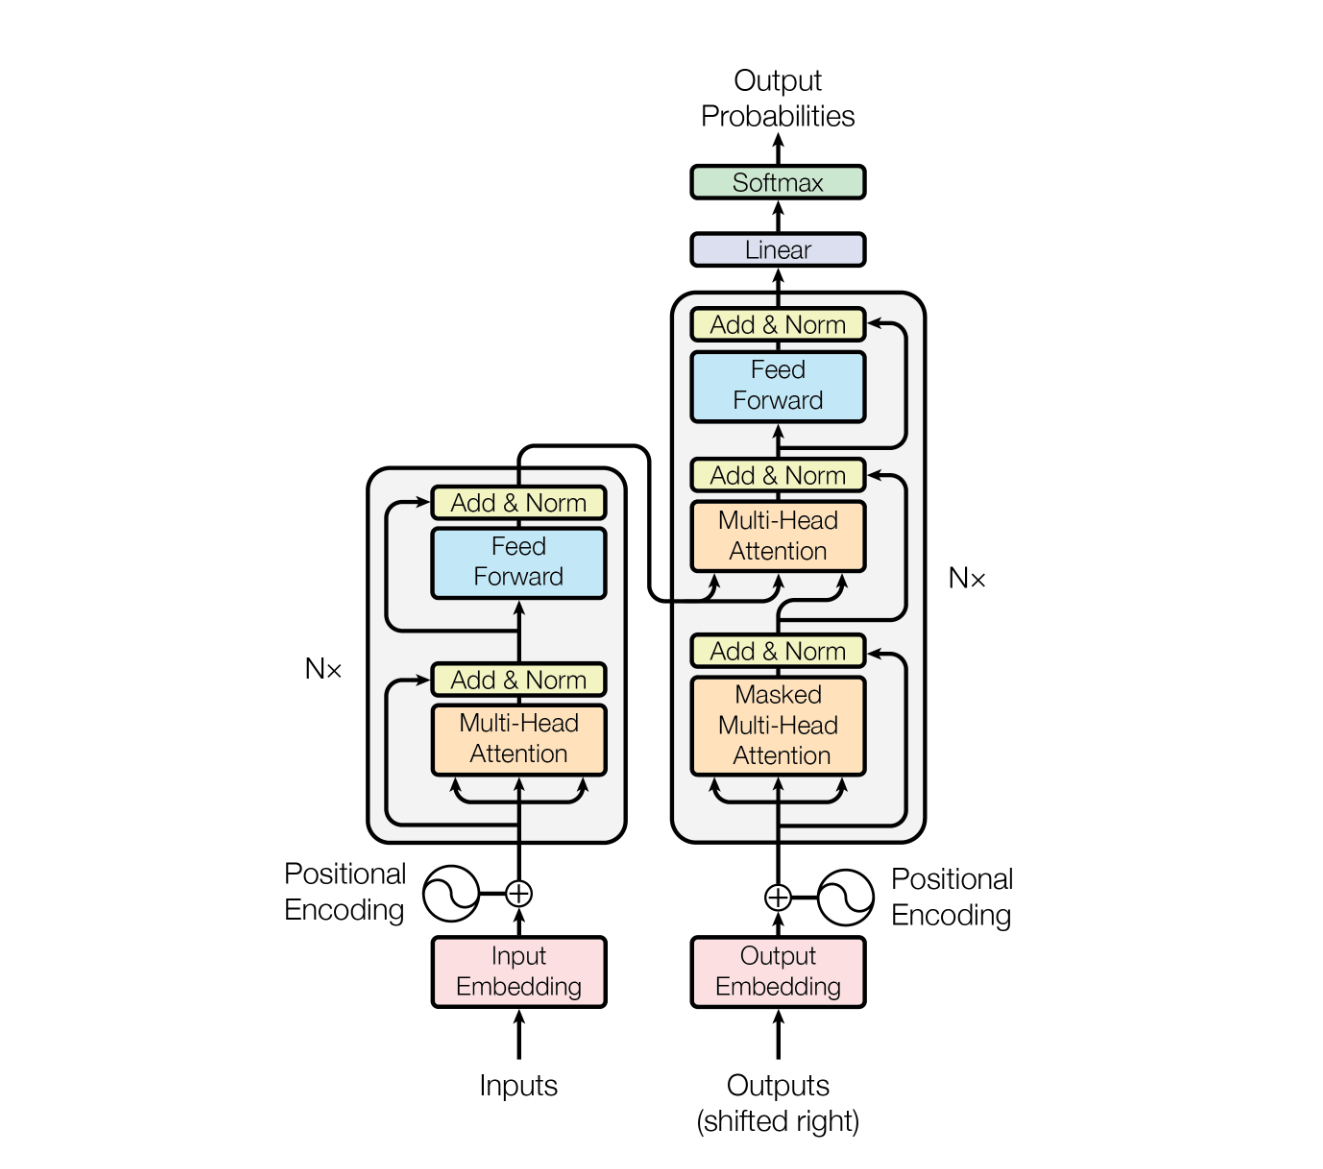
\includegraphics[width=0.8\textwidth]{images/transformer.png}
    \caption{Architettura Transformer.}
    \label{fig:transformer}
\end{figure}

































\chapter{Analisi dei dati raccolti}\label{cap:analisi_dati}

Questo capitolo tratterà in maniera preliminare le modalità con cui si è deciso di strutturare il dataset \emph{SciLay} creato. Questa panoramica serve da introduzione per contestualizzare il lavoro futuro, mentre i dettagli verranno affrontati nei capitoli successivi. 

\section{Origine e creazione del dataset}
Come anticipato nell'introduzione, nel panorama scientifico attuale vi è una forte carenza di articoli che dispongano di lay summary. Probabilmente a causa di questo vuoto, in letteratura è raro trovare dataset preesistenti che includano decine di migliaia di documenti provenienti da differenti riviste. Di conseguenza, è sorta l'esigenza di crearne uno su misura. Opera, questa, di non semplice realizzazione per via di tale carenza, richiedendo un'attenta selezione e cura dei dati disponibili.
La prima fase di questo progetto ha implicato un'accurata analisi delle riviste scientifiche che proponessero lay summary, così come elencate sul sito di KTDRR. La ricerca, purtroppo, ha portato a risultati non ottimali rispetto agli obbiettivi preposti. Numerose riviste limitavano l'accesso ai loro articoli mediante sottoscrizioni, mentre quelle che offrivano accessi gratuiti presentavano una disponibilità estremamente limitata, spesso circoscritta a 100-200 articoli per ogni rivista. Tra le fonti più rilevanti, si annoverano \href{https://onlinelibrary.wiley.com/}{Wiley-Journal}, \href{https://www.cochranelibrary.com/cdsr/reviews}{Cochrane}, \href{https://www.pnas.org/}{PNAS}, \href{https://www.journalslibrary.nihr.ac.uk/#/}{NIHR} e \href{https://journals.plos.org/plosmedicine/issue?id=10.1371/issue.pmed.v20.i01}{PLoS Medicine}. 
Una problematica addizionale è stata la predominanza del formato PDF tra le pubblicazioni, un formato notoriamente complesso da analizzare\footnote{Diverse metodologie sono state esplorate, tra cui l'uso di librerie standard come PyPDF2 e l'impiego di soluzioni AI, come Grobid e Science Parser, con quest'ultima che ha fornito i migliori risultati.}. 
In risposta a tali difficoltà, si è valutata l'opportunità di adottare un diverso approccio metodologico, privilegiando formati più agevolmente analizzabili. Sebbene l'idea iniziale fosse orientata verso il web scraping delle pagine HTML degli articoli, la mancanza di standardizzazione tra le pagine delle varie riviste ha reso l'approccio non fattibile.
Fortunatamente, ulteriori indagini hanno condotto alla scoperta di un database fornito da \href{https://pubmed.ncbi.nlm.nih.gov/}{PubMed}, che proponeva articoli in formato XML disponibili per il \href{https://ftp.ncbi.nlm.nih.gov/pub/pmc/oa_bulk/oa_comm/}{download massivo}. Una volta acquisiti, si è notato che tali documenti presentavano una struttura uniforme, rendendo possibile una raccolta sistematica dei dati rilevanti, riuscendo a filtrare le parti rilevanti per lo scopo del progetto.


\section{Caratteristiche principali} 
Dall'analisi di diversi articoli, è stato generato un dataset composto da $43,790$ istanze.  Di seguito è descritta nel dettaglio la struttura scelta per il dataset in questione.

\subsection{Struttura delle istanze}
Ciascuna delle $43,790$ istanze presenta la seguente struttura:
\begin{itemize}
    \item \textbf{DOI}. Standard internazionale utilizzato per garantire l'identificazione duratura e univoca di oggetti digitali di varia natura. Il DOI è adottato per identificare ciascuna istanza del dataset prodotto, fornendo un collegamento diretto ai metadati associati all'articolo di riferimento.
    \item \textbf{PMCID}. Identificativo univoco all'interno del database di PMC (PubMed Central, libreria open access di PubMed). L'uso del PMCID facilita l'accesso e la navigazione all'interno di PMC, permettendo di localizzare specifici articoli senza necessariamente fare riferimento al DOI.
    \item \textbf{Plain Text}. Questo campo corrisponde al lay summary, ovvero un riassunto accessibile e comprensibile dell'articolo in esame.
    \item \textbf{Technical Text}. Si riferisce all'abstract dell'articolo, fornendo una sintesi tecnica dei contenuti presentati.
    \item \textbf{Full Text}. Rappresenta l'intero contenuto dell'articolo scientifico.
    \item \textbf{Journal}. Indica la rivista scientifica in cui l'articolo è stato pubblicato. Questa informazione fornisce uno sfondo sul contesto e la reputazione della fonte di ricerca. Si noterà che, in questa tesi, il dataset viene analizzato anche in base alle singole riviste di pubblicazione.
    \item \textbf{Topics}. Categorizzazione dell'articolo in base alla sua natura, come ad esempio se è una ricerca, una review o altri tipi di pubblicazioni.
    \item \textbf{Keywords}. Le parole chiave associate all'articolo, utili per definire e contestualizzare l'ambito e il focus del documento.
\end{itemize}
\subsection{Suddivisione in subset per rivista}
Come anticipato, il dataset è anche stato suddiviso in subset a seconda del giornale di appartenenza. Questa modalità di lavoro presenta una serie di benefici chiave che consentono di condurre esperimenti più attendibili e generalizzabili. 
In primo luogo questo sistema tiene conto della \emph{specificità delle riviste}: ogni rivista può avere uno stile, un focus o una specializzazione unici. Suddividendo il dataset per rivista, è possibile analizzare e comprendere meglio queste specificità. Un ulteriore vantaggio offerto da questa metodologia è la possibilità di implementare una \emph{validazione incrociata}. Questa tecnica prevede l'addestramento di un modello su uno o più subset, per poi valutare le sue prestazioni su subset differenti. Questo approccio non solo assicura una maggiore robustezza dei risultati ottenuti, ma consente anche di verificare l'efficacia e l'applicabilità del modello in diversi contesti editoriali.
Infine, l'adozione di questa strategia di suddivisione facilita l'addestramento di \emph{modelli specifici} per ciascuna rivista. Grazie a tale specializzazione, è possibile ottimizzare le prestazioni del modello rispetto allo stile e alla terminologia propri di una determinata rivista, garantendo risultati di elevata qualità e pertinenza.
In sintesi, la segmentazione del dataset in base al giornale di appartenenza si rivela un approccio strategico e metodologico di fondamentale importanza per garantire la validità e la rilevanza delle analisi condotte.
Più nel concreto, a seguito dell'analisi delle istanze collezionate, si è deciso di generare dei subset solamente laddove la rivista fornisse un numero di istanze che fosse $\geq 1\%$ rispetto al numero di articoli totali. Questo per evitare di avere split con un numero di istanze irrisorio. Oltre a questo è stata ovviamente messo a disposizione l'intero dataset. 
La Figura \ref{fig:journal-inst-perc} mostra la distribuzione percentuale delle istanze per ogni rivista rispetto al totale. La voce ``\emph{Others}'' corrisponde all'insieme delle riviste con istanze insufficienti per avere un subset autonomo.

\begin{figure}
    \centering
    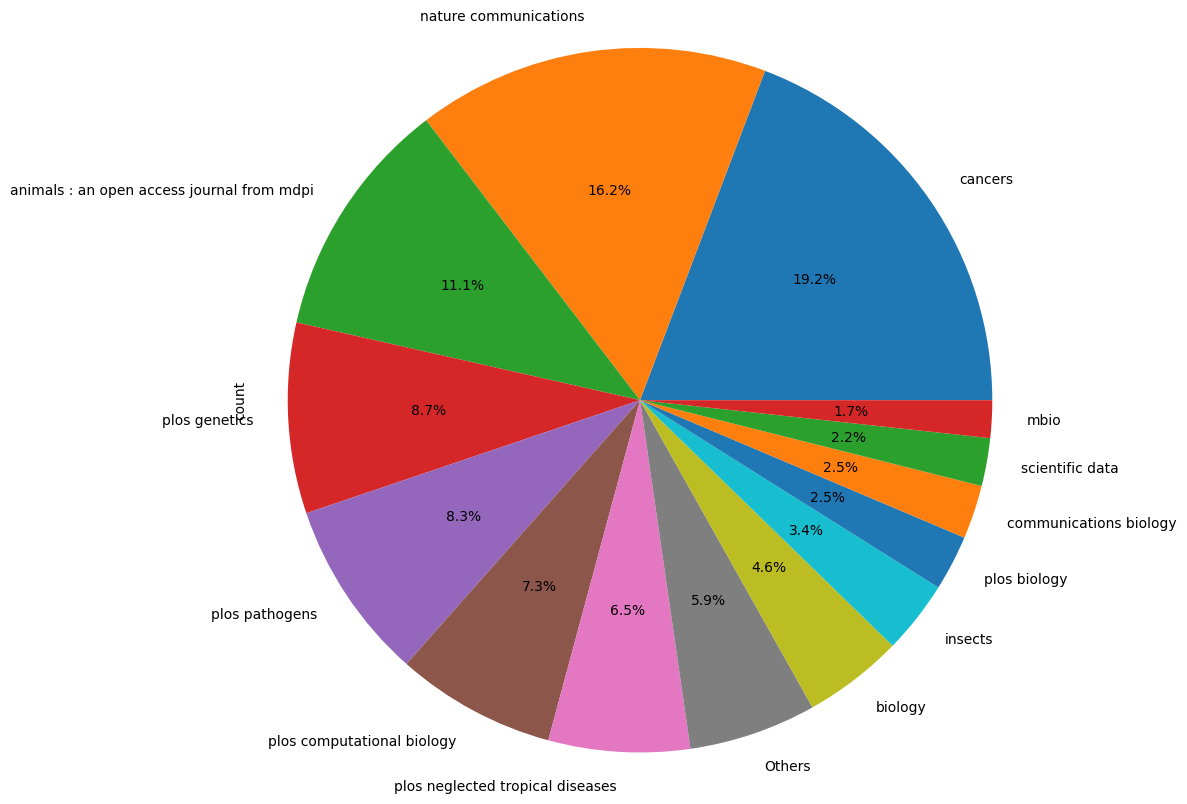
\includegraphics[width=\textwidth]{images/journal_instances_percentage.png}
    \caption{Distribuzione percentuale delle istanze per rivista.}
    \label{fig:journal-inst-perc}
\end{figure}


La suddivisione ha seguito fedelmente la distribuzione mostrata nella figura in questione, cioè si sono generati 13 subset oltre a quello che comprende le riviste con meno istanze. 
La tabella \ref{tab:split-journals} mostra in termini numerici la dimensione di ogni subset.

\begin{table}
\centering
\begin{tabular}{|l|c|c|c|}
\hline
       & train & validation & test \\
\hline
all    & 35026 & 4380       & 4384 \\
NC     & 5549  & 694        & 694  \\
A      & 3909  & 489        & 489  \\
PLGEN  & 3087  & 386        & 386  \\
PLPAT  & 2920  & 365        & 365  \\
PLCB   & 2589  & 324        & 324  \\
PLNTD  & 2289  & 286        & 287  \\
B      & 1617  & 202        & 203  \\
I      & 1181  & 148        & 148  \\
PLB    & 896   & 112        & 113  \\
CB     & 867   & 108        & 109  \\
SD     & 725   & 91         & 91   \\
MBIO   & 607   & 76         & 76   \\
C      & 6782  & 848        & 848  \\
OTHER  & 2008  & 251        & 251  \\
\hline
\end{tabular}
\caption{Dimensione numerica di ogni subset.}
\label{tab:split-journals}
\end{table}

Per questioni di sintesi, i nomi delle riviste sono stati abbreviati come segue:
\begin{itemize}
    \item NC: Nature Communications.
    \item A: Animals : An Open Access Journal from MDPI.
    \item PLGEN, PLAPAT, PLCB, PLNTD, PLB: PLoS \{Genetics, Pathogens, Computational Biology, Neglected Tropical Diseases, Biology\}.
    \item B: Biology.
    \item I: Insects.
    \item CB: Communications Biology.
    \item SD: Scientific Data.
    \item MBIO: mBio.
    \item C: Cancers.
\end{itemize}


\section{Upload del dataset su HuggingFace}
Come ultima operazione effettuata sui dati, si è deciso di caricare l'intero dataset su \href{https://huggingface.co/}{\emph{HuggingFace}} nel repository intitolato, per l'appunto, \href{https://huggingface.co/datasets/paniniDot/sci_lay}{\emph{sci\_lay}}. 
Hugging Face è diventata una delle principali piattaforme per il Natural Language Processing (NLP) e il Deep Learning, offrendo un'ecosistema completo per la formazione, il testing e la distribuzione di modelli di linguaggio. Caricare un dataset su Hugging Face può offrire una serie di vantaggi chiave, in particolare per la comunità di ricercatori e sviluppatori. Ecco una descrizione dei motivi principali:

\begin{itemize}
    \item \textbf{Accessibilità}: Una volta caricato su Hugging Face, il dataset diventa facilmente accessibile a chiunque nella comunità. Questo permette ad altri ricercatori e sviluppatori di sfruttare il dataset senza passare attraverso processi di download e setup complicati.
    \item \textbf{Standardizzazione}: Hugging Face offre una struttura standardizzata per i dataset, rendendo più semplice per gli utenti navigare, comprendere e utilizzare diversi dataset in modo coerente. 
    \item \textbf{Integrazione con Modelli}: Hugging Face non è solo una piattaforma per dataset, ma anche per modelli di linguaggio. Caricando un dataset lì, si facilita la formazione, il fine-tuning e la valutazione dei modelli usando quella specifica risorsa, tutto all'interno dello stesso ecosistema.
    \item \textbf{Versioning}: Proprio come per i software, i dataset possono subire modifiche e revisioni nel tempo. Hugging Face supporta il versioning, permettendo agli utenti di accedere a diverse versioni del dataset e tracciare le modifiche. Nel caso di SciLay, ad esempio, il dataset è disponibile solo nella versione $1.0.0$ (cased) che dispone degli articoli con caratteri maiuscoli e minuscoli.
    \item \textbf{Documentazione e Metadati}: La piattaforma permette di fornire documentazione dettagliata, basata sul concetto di \emph{Dataset Card} proposta nell'articolo ``Data Cards: Purposeful and Transparent Dataset Documentation for Responsible AI''\cite{pushkarna2022data}, e metadati associati al dataset. In questo modo si aiutano gli utenti a comprendere e utilizzare al meglio la risorsa.
\end{itemize}

In conclusione, caricare un dataset su Hugging Face non solo semplifica la distribuzione e l'adozione della risorsa, ma promuove anche la standardizzazione, la collaborazione e l'innovazione nell'ambito del Natural Language Processing e delle discipline correlate. 






















\chapter{Modellazione del progetto}
\label{cap:modellazione-prog}

Mentre i capitoli precedenti hanno approfondito l'esplorazione delle tecnologie esistenti e l'analisi dei dati, questo capitolo funge da collegamento cruciale tra la teoria e la pratica, offrendo uno sguardo approfondito sulla modellazione effettiva del progetto.
In questo capitolo discuteremo le decisioni di design del nostro sistema, le scelte di modellazione intraprese e come le tecnologie appena introdotte possano essere adattate e ottimizzate per affrontare il problema in questione. 


\section{Infrastruttura e Risorse}

Fin dal primo momento ci si è trovati di fronte alla sfida di eseguire esperimenti su modelli con una notevole complessità computazionale. 
Al giorno d'oggi, infatti, anche i modelli di intelligenza artificiale più basilari richiedono una potenza di elaborazione che solo GPU di alta qualità possono fornire.
A questo proposito il professor Moro ha generosamente offerto l'accesso al suo server, garantendomi una capacità di calcolo che non avrei potuto ottenere altrimenti.
Il server dispone infatti di sei NVIDIA GeForce GTX 3090 da 24GiB di VRAM e altre GeForce GTX TITAN XP da 12GiB di VRAM.

Data la posizione fisica remota del server e il fatto che sia condiviso con altri tesisti e ricercatori, si è resa necessaria una gestione accurata delle risorse in un contesto di utilizzo condiviso. Queste considerazioni hanno guidato l'adozione di tecnologie come:
\begin{itemize}
    \item \emph{Slurm}
    \item \emph{Docker}
    \item \emph{SSH}
\end{itemize}
che verranno trattate nel dettaglio nelle sottosezioni successive.

\subsection{Docker}

Docker è una piattaforma software open-source che consente di creare, eseguire e gestire applicazioni all'interno di contenitori (anche detti \emph{container}). Un \emph{container} è una unità standardizzata di software che racchiude il codice e tutte le sue dipendenze in modo che l'applicazione possa essere eseguita in modo uniforme e coerente su qualsiasi ambiente. Questi contenitori sono leggeri, dato che non richiedono l'overhead di una macchina virtuale completa, ma si avvalgono dello stesso kernel del sistema operativo sottostante. 

\subsubsection{Perché scegliere Docker su una VM}
Come anticipato, una delle principali differenze fra un sistema di containerizzazione e una virtual machine (VM) è il fatto che ogni contenitore si appoggia sul sistema operativo della macchina in cui viene eseguito, come mostrato in figura \ref{fig:docker-vm}. 

\begin{figure}
    \centering
    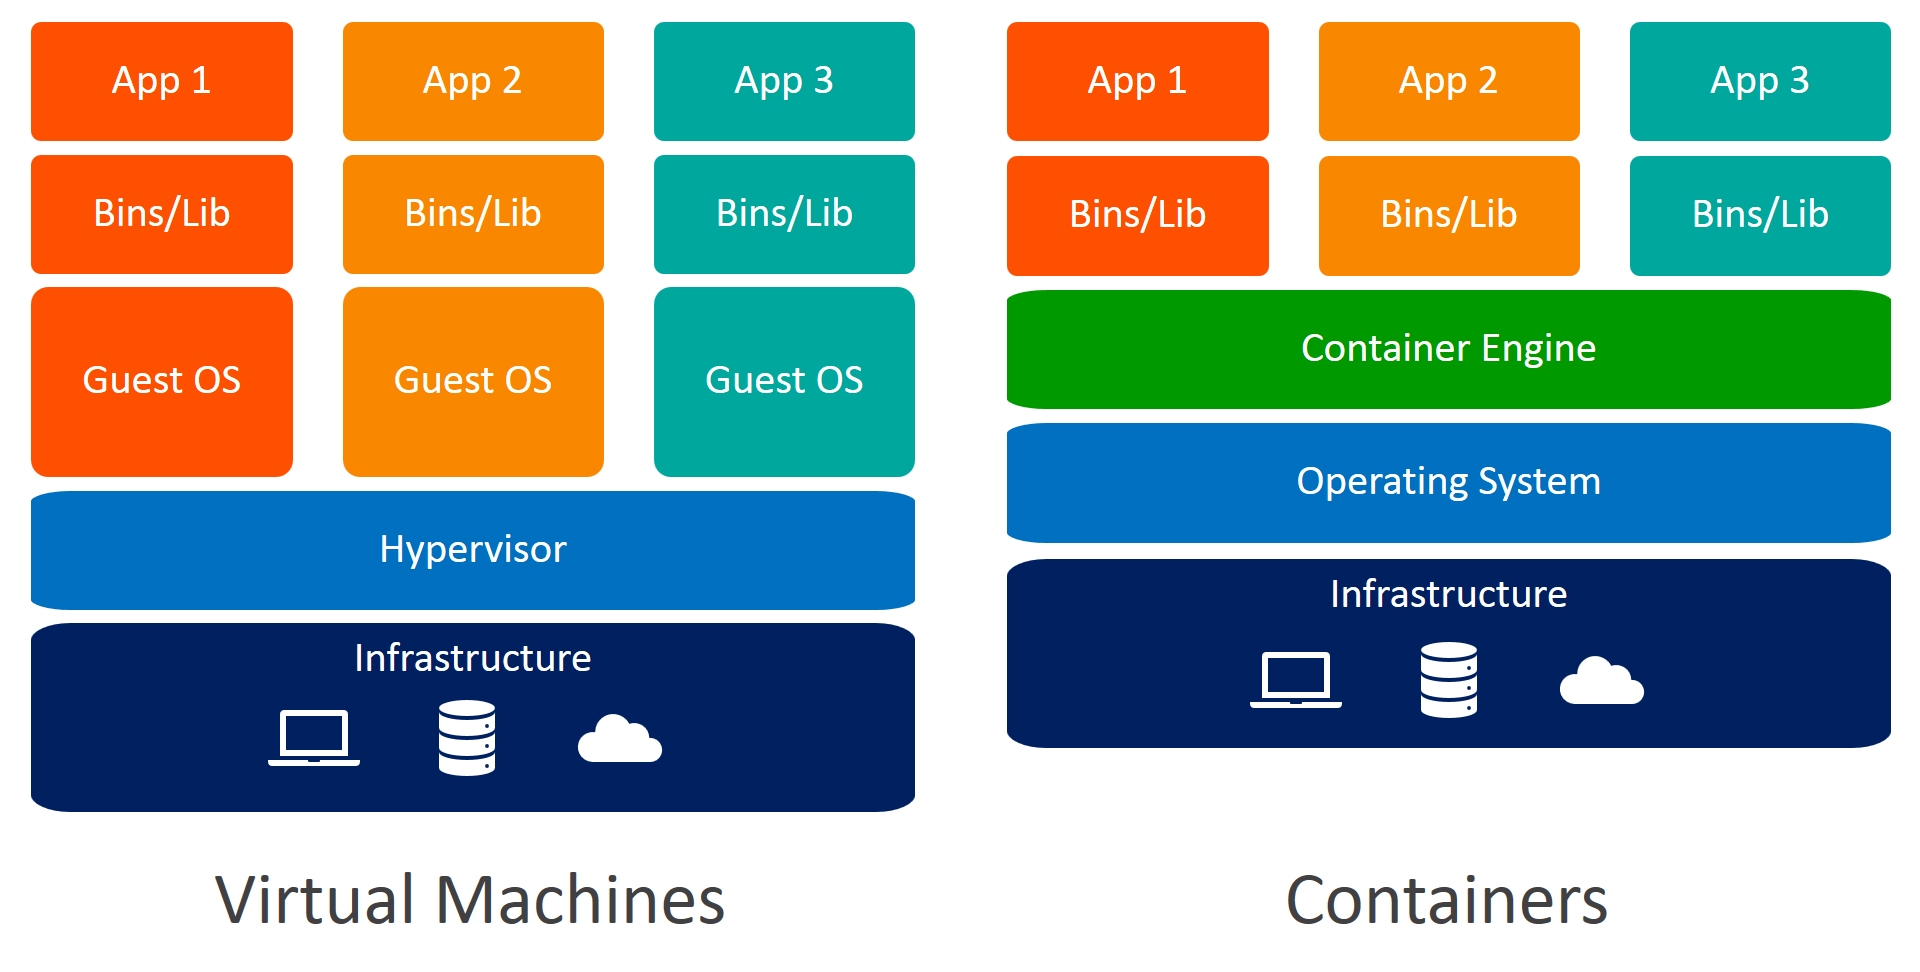
\includegraphics[width=0.9\textwidth]{images/container-vm.png}
    \caption{Confronto fra stack VM e container.}
    \label{fig:docker-vm}
    \tiny{Fonte: https://images.contentstack.io/v3/assets/blt300387d93dabf50e/bltb6200bc085503718/5e1f209a63d1b6503160c6d5/containers-vs-virtual-machines.jpg}
\end{figure}

Questa semplice differenza comporta una serie di vantaggi risultati essenziali, fra i principali si riportano

\begin{itemize}
    \item \emph{Leggerezza}. I container condividono lo stesso sistema operativo (OS) host, mentre ogni VM ha il proprio sistema operativo completo. Questo significa che i container tendono a utilizzare meno risorse rispetto alle VM.
    \item \emph{Avvio più veloce}. Poiché i container non hanno bisogno di avviare un intero sistema operativo, possono essere avviati in pochi secondi, mentre le VM potrebbero richiedere minuti.
    \item \emph{Maggiore densità}. Grazie alla loro leggerezza, è possibile eseguire molti più container su un host rispetto a quante VM potrebbero essere eseguite sulla stessa infrastruttura. 
    \item \emph{Portabilità}. I container sono progettati per essere portatili. Con tecnologie come Docker, è possibile "containerizzare" un'applicazione con tutte le sue dipendenze e eseguirla in modo coerente su diversi ambienti, dallo sviluppo alla produzione.
    \item \emph{Scalabilità}. La capacità di avviare rapidamente i container li rende ideali per soluzioni scalabili, dove nuove istanze di un'applicazione devono essere avviate o fermate rapidamente in risposta al carico.
\end{itemize}


\subsubsection{Isolamento e Riproducibilità}
Le due caratteristiche di fondamentale importanza per lo svolgimento di questo progetto sono l'\emph{isolamento} e la \emph{riproducibilità}. Poiché il cluster condiviso di GPU poneva il problema di mantenere dei blocchi funzionali indipendenti dal nodo in uso, che contenessero tutto il necessario per poter eseguire del codice di deep learning, Docker si è rivelato di vitale importanza. In particolare poiché fornisce
\begin{itemize}
    \item \emph{Ambienti di lavoro isolati}. Docker consente di creare contenitori che funzionano in modo isolato dal sistema host e dagli altri contenitori,garantendo che le risorse, come la CPU, la memoria e la GPU, assegnate a un contenitore non interferiscano con altri contenitori o con il sistema host. In un ambiente clusterizzato, ciò è essenziale per garantire che ogni job riceva le risorse di cui ha bisogno senza conflitti.
    \item \emph{Riproducibilità}. Una delle sfide principali nella ricerca scientifica è assicurarsi che gli esperimenti siano riproducibili. Grazie alle immagini Docker, è possibile specificare esattamente quali software, librerie e versioni sono necessarie. Questo significa che, fornendo il container (o l'\emph{immagine} da cui crearlo), l'ambiente di esecuzione rimarrà lo stesso indipendentemente dall'host sul quale viene eseguito, garantendo così la riproducibilità degli esperimenti.

    \item \emph{Gestione delle dipendenze}. In un contesto di sperimentazione di baseline di abstractive summarization è essenziale scegliere le dipendenze (nonché le versioni) giuste. Docker consente di semplificare questa gestione. Ad esempio, se il progetto richiedeva una versione specifica di una libreria per la GPU o una particolare versione di una libreria di elaborazione del linguaggio naturale, queste potevano essere specificate nel \emph{Dockerfile}. Questo ha eliminato i problemi derivanti dall'avere versioni diverse delle dipendenze installate su nodi diversi del cluster.
\end{itemize}


\subsubsection{Dockerfile e immagini}

Docker si basa su tre concetti fondamentali per implementare il suo approccio alla containerizzazione, come mostrato in figura \ref{fig:docker-uml}. Questi concetti sono:
\begin{itemize}
    \item Dockerfile
    \item Immagini
    \item Containers
\end{itemize}
Il \emph{Dockerfile} rappresenta una ricetta testuale che Docker utilizza per creare immagini di container. Esso dettaglia una sequenza di istruzioni che Docker segue passo dopo passo. È interessante notare che un singolo Dockerfile può dar vita a diverse immagini.

L'\emph{Immagine} è essenzialmente un pacchetto eseguibile che racchiude tutto ciò che serve per far funzionare un'applicazione: dal codice, alle librerie, alle variabili di ambiente, fino ai file di configurazione.

Il \emph{Container}, d'altra parte, è una versione eseguibile di un'immagine. Quando un'immagine viene avviata, essa prende vita sotto forma di container. Questi container funzionano in maniera isolata, sia tra loro sia rispetto al sistema host, garantendo che ogni container abbia le proprie risorse, come filesystem, connessione di rete e identificatori di processo (PID).

Il flusso di lavoro (anch'esso sintetizzato in Figura \ref{fig:docker-uml}) tipico con Docker include la scrittura di un Dockerfile, la costruzione di un'immagine da quel Dockerfile e, infine, l'esecuzione di un container basato sull'immagine costruita.

Come anticipato, durante la fase di modellazione del progetto, l'adozione di Docker è stata decisiva per assicurare coerenza e riproducibilità nell'ambiente di esecuzione. 
Visto che il dataset \emph{SciLay} è stato pubblicato su HuggingFace, per garantire consistenza, abbiamo optato per l'utilizzo delle API fornite da HuggingFace attraverso la libreria \texttt{Transformers}. Di conseguenza, nella creazione del Dockerfile, ci siamo appoggiati all'immagine base ``\href{https://hub.docker.com/r/huggingface/transformers-pytorch-gpu/}{huggingface/transformers-pytorch-latest-gpu}'', che fornisce le librerie essenziali di PyTorch e Hugging Face Transformers per GPU, garantendo così la massima efficienza nell'addestramento e nell'inferenza dei modelli.

Oltre a questo, volendo provare i \emph{Large Language Models (LLM)} più recenti come \emph{LLama2} e \emph{Mistral}, si è posta la necessità di avere un container fortemente ottimizzato per le GPU Nvidia a nostra disposizione. Per questo motivo si è deciso di partire da immagini fornite da Nvidia stessa come ``\href{https://docs.nvidia.com/deeplearning/frameworks/pytorch-release-notes/rel-22-12.html}{nvcr.io/nvidia/pytorch:22.12-py3}''. Questo fornisce accesso alle libreria CUDA 11.8, le quali rimangono retrocompatibili con le GPU a nostra disposizione (limitate a CUDA 11.6) pur dando la possibilità di usare l'ultima versione di \texttt{PyTorch}.

\begin{figure}
    \centering
    \begin{minipage}{\textwidth}
        \centering
        \begin{tikzpicture}[node distance=3.0cm, font=\small, scale=0.75, every node/.style={transform shape}]
            % Classi
            \node (dockerfile) [draw, rectangle, minimum width=3cm, minimum height=1.5cm] {Dockerfile};
            \node (immagine) [draw, rectangle, minimum width=3cm, minimum height=1.5cm, below of=dockerfile] {Immagine};
            \node (container) [draw, rectangle, minimum width=3cm, minimum height=1.5cm, below of=immagine] {Container};
            
            % Associazioni
            \draw (dockerfile.south) -- node[right, very near start] {1} node[right, very near end] {0..*} node[left, midway] {build} (immagine.north);
            \draw (immagine.south) -- node[right, very near start] {1} node[right, very near end] {0..1} node[left, midway] {run} (container.north);
        \end{tikzpicture}
    \end{minipage}

    \vspace{1cm}

    \begin{minipage}{\textwidth}
        \centering
        \scalebox{0.75}{
            \begin{sequencediagram}
  \newthread{df}{\texttt{Dockerfile}}
  \newinst[3]{img}{\texttt{Immagine}}
  \newinst[3]{ctr}{\texttt{Container}}

  \begin{call}{df}{Build}{img}{}
    \begin{call}{img}{Run}{ctr}{}
    \end{call}
  \end{call}
\end{sequencediagram}
        }
    \end{minipage}
    \caption{Diagrammi delle classi (in alto) e di sequenza (in basso) mostranti le relazioni statiche e dinamiche tra Dockerfile, Immagine e Container.}
    \label{fig:docker-uml}
\end{figure}

\subsection{Slurm}

\emph{Slurm} è un sistema open source per la gestione di cluster e la pianificazione di lavori, ideale sia per grandi che piccoli cluster Linux. È resistente ai guasti, altamente scalabile e non richiede modifiche al kernel per funzionare. Slurm svolge tre funzioni principali come gestore di carichi di lavoro su cluster:

\begin{enumerate}
    \item Assegna l'accesso esclusivo o condiviso alle risorse (nodi di calcolo) agli utenti per un certo periodo di tempo, permettendo loro di eseguire operazioni.
    \item Offre una struttura per avviare, eseguire e monitorare lavori, solitamente paralleli, sui nodi assegnati.
    \item Gestisce una coda di lavori in attesa, arbitrando l'accesso alle risorse.
\end{enumerate}

\subsubsection{Architettura}
Come mostrato in Figura \ref{fig:slurm-arch}, Slurm utilizza un gestore centralizzato, chiamato \textbf{slurmctld}, per monitorare risorse e lavori. Può anche esserci un gestore di backup pronto a sostituirlo in caso di guasto. Ogni server di calcolo (o nodo) ha un demone chiamato \textbf{slurmd}, che funziona un po' come una shell remota: attende istruzioni, le esegue, restituisce lo stato e attende altre istruzioni. 

Esiste un demone opzionale, \textbf{slurmdbd}, che registra informazioni contabili (i.e. monitoraggio delle risorse) per più cluster gestiti da Slurm in un unico database. Esistono anche altri componenti che però verranno trascurati per ragioni di semplicità. 

\begin{figure}
    \centering
    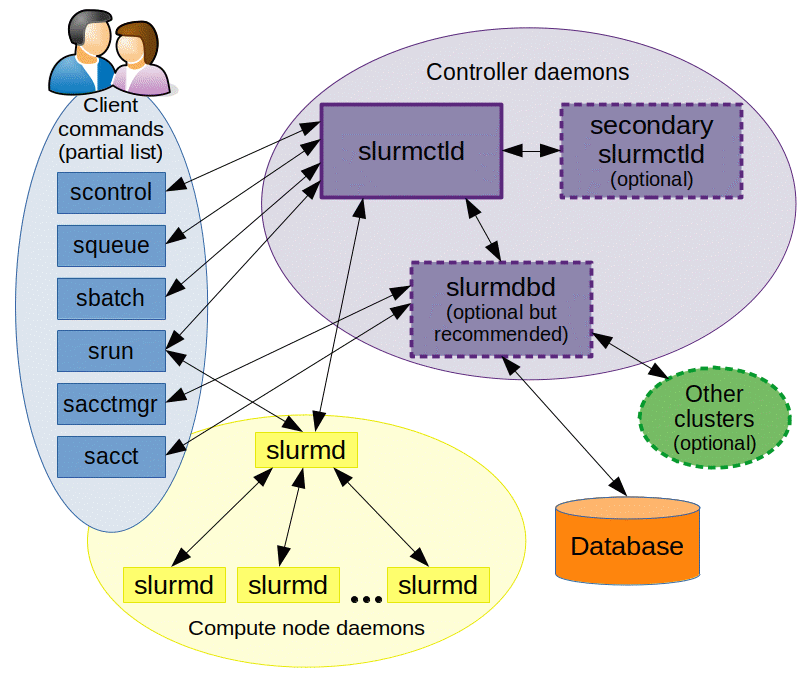
\includegraphics[width=0.6\textwidth]{images/slurm-architecture.png}
    \caption{Architettura di Slurm.}
    \label{fig:slurm-arch}
    \tiny{Fonte: https://slurm.schedmd.com/overview.html}
\end{figure}

Ogni client può agire sia sul controller centrale (\textbf{slurmctld}) che sui CLI associate a ciascun nodo (\textbf{slurmd}), lanciando diversi comandi, fra cui
\begin{itemize}
    \item \emph{srun}: per avviare jobs in modalità interattiva;
    \item \emph{sbatch}: per avviare jobs in batch;
    \item \emph{scancel}: per terminare lavori in coda o in esecuzione;
    \item \emph{sinfo}: per riportare lo stato del sistema;
\end{itemize}

Nello specifico, nel cluster di GPU utilizzato, all'atto dell'inserimento di un task in coda, viene calcolato un valore intero per definirne la priorità. Questo valore tiene conto di diversi fattori, tra cui l'ordine di inserimento e il bilanciamento di carico tra gli utenti.

\subsubsection{Parallelizzazione e Gestione delle Risorse}
Nonostante la capacità di Slurm di gestire complessi cluster multi-nodo, si è optato per un approccio semplice ma efficace, utilizzando sempre un singolo nodo per ogni esperimento. Questo ha permesso di avere un controllo totale sulla GPU desiderata e di garantire che ogni esperimento avesse accesso esclusivo alle risorse necessarie.

Nella fase di configurazione dei task, si è preferito adottare un approccio ibrido tra interazione diretta con l'utente ed esecuzione autonoma (in batch) degli esperimenti. A tal proposito, Slurm mette a disposizione due comandi fondamentali: \emph{srun} e \emph{sbatch}. Mentre \emph{sbatch} si rivela la scelta ideale per esperimenti di lunga durata che non necessitano di interventi manuali, nelle fasi iniziali del progetto \emph{srun} risulta essere estremamente utile.
Il valore aggiunto di \emph{srun} è la sua capacità di avviare sessioni in modalità interattiva. Questo permette di lanciare un lavoro e, contemporaneamente, di accedere a una shell direttamente nel nodo assegnato. Tale funzionalità si è rivelata particolarmente preziosa per operazioni di debugging, per condurre test in maniera agile o per analizzare i dati in tempo reale. Una volta che il codice è stato ottimizzato e testato, per gli addestramenti prolungati e stabili, si è fatto affidamento su \emph{sbatch}.

Questo approccio, pur essendo semplice, si è dimostrato efficace per le esigenze di questo progetto. Si è potuto sfruttare la potenza del cluster di GPU mantenendo al contempo un elevato livello di controllo e prevedibilità. La combinazione di Slurm con il metodo di utilizzo appena descritto ha permesso di eseguire gli esperimenti in modo efficiente, garantendo risultati tempestivi e affidabili.

\subsection{Flusso di lavoro complessivo}
Complessivamente, come mostrato in Figura \ref{fig:seq-cluster}, il flusso di lavoro prevede una fase di connessione al server via SSH (Secure SHell) mediante credenziali fornite dall'amministratore del cluster, Giacomo Frisoni. Una volta connessi e configurata una shell byobu (il cui vantaggio è quello di garantire \emph{shell persistenti}, cioè che rimangano attive anche dopo la chiusura del CLI), data la condivisione delle risorse, si procede inserendosi in una coda di attesa gestita da Slurm. Una volta ottenute le risorse necessarie (cioè è stato allocato un nodo), si porcede con l'avvio degli esperimenti all'interno di specifici container grazie a Docker. Per fare questo, prima è necessario aver creato un'immagine a partire dal Dockerfile,  dunque formalmente avviene il controllo mostrato in figura.
All'interno del container, una volta istanziato, si esegue uno script sh che lancia un programma python passandogli dei parametri che andranno definiti in fase di sviluppo del progetto.

\begin{figure}
\centering
\scalebox{0.65}{
\begin{sequencediagram}
    \newthread{user}{User}
    \newinst[3]{slurm}{Slurm Node (GPU)}
    \newinst[3]{image}{Image}
    \newinst[3]{container}{Container}

    \begin{call}{user}{connect(ip, port, login)}{slurm}{}
    \end{call}
    \begin{call}{user}{srun/sbatch}{slurm}{}
        \begin{sdblock}{Opt[if does not exist]}{}
            \begin{call}{slurm}{build image}{image}{}
            \end{call}
        \end{sdblock}
        \begin{call}{slurm}{start container}{container}{Container code executed}
            \begin{call}{container}{Run Script}{container}{Script executed}
            \end{call}
        \end{call}
    \end{call}
\end{sequencediagram}
}
\caption{Diagramma di sequenza per la gestione del cluster di GPU.}
\label{fig:seq-cluster}
\end{figure}


\subsubsection{Considerazioni pratiche}
Una complicazione è emersa dal fatto che Slurm percepisce ogni nodo come se fosse un componente della stessa unità computazionale. Di conseguenza, richiedendo risorse da un nodo, potrebbero venire allocate su un altro. Per garantire che gli esperimenti vengano eseguiti correttamente, è fondamentale che il codice su ogni macchina ri1manga sincronizzato. Sebbene esistano strumenti dedicati alla sincronizzazione dei file, come Unison, una soluzione efficace è mantenere tutto all'interno di un repository Git, metodo adottato per questo progetto.


\section{Architettura del sistema}
Le recenti innovazioni nel campo del deep learning, in particolare nell'ambito dell'NLP, hanno portato alla creazione di modelli di summarization \emph{astrattivi} che superano ampiamente le performance delle tecniche \emph{estrattive} precedentemente adottate. Da questa constatazione, l'attenzione si è spostata verso questo tipo di approcci, capaci di interpretare in modo più profondo il contenuto dei testi e di generare sintesi più accurate, evitando le carenze tipiche dei modelli estrattivi come la frammentazione e la mancanza di fluidità nel riassunto.

Considerando la vastità di tecniche astrattive, come discusso nel capitolo \ref{cap:tecnologie}, è emerso che i modelli basati sull'architettura encoder-decoder RNN presentano delle limitazioni. Una delle loro principali debolezze risiede nella gestione di testi lunghi: di fronte a testi estesi, tendono a troncare il contenuto, limitando la capacità di generare riassunti completi. Questa limitazione è particolarmente critica quando si tratta di documenti come quelli di SciLay, che sono di notevole lunghezza e contengono informazioni rilevanti sparse in tutto il testo.

In questo contesto, l'architettura Transformer si è distinta come soluzione promettente. Questi modelli non solo superano i modelli RNN in termini di accuratezza, ma hanno anche dimostrato di essere particolarmente efficaci nell'analisi di testi lunghi, grazie alla loro capacità di comprendere relazioni a distanza nel testo. Di conseguenza, la scelta è stata quella di basare il nostro sistema esclusivamente su questa architettura.

\section{Scelte di modellazione}
Per i nostri esperimenti sono state utilizzate delle \emph{baseline astrattive}. Questo significa che sono stati selezionati i modelli più promettenti disponibili in letteratura senza effettuare fine-tuning degli iperparametri. La descrizione dei modelli è stata categorizzata in base alla loro architettura sottostante ma sono tutti accomunati dall'utilizzo di transformers piuttosto che RNN.

\subsection{Modelli Seq2Seq con Attention}
I modelli Seq2Seq con Attention sono stati ampiamente descritti nel capitolo \ref{cap:tecnologie}. Tra questi, i più noti sono 
\begin{itemize}
    \item BART
    \item T5
    \item PEGASUS
\end{itemize}
tutti basati sull'architettura a Transformers.

\subsubsection{Bart}
\emph{BART} (Bidirectional and Auto-Regressive Transformer) \cite{DBLP:journals/corr/abs-1910-13461} di Facebook AI è stato progettato per compiti di elaborazione del linguaggio naturale (NLP), come il riassunto e la correzione grammaticale. Il suo metodo di pre-addestramento, \emph{denoising autoencoder}, altera il testo in ingresso in vari modi e poi tenta di ricostruirlo attraverso un approccio \emph{auto-regressivo}. BART è disponibile in diverse varianti, tra cui \emph{base} e \emph{large}, come riassunto nella Tabella \ref{tab:bart-comparison}. Sebbene la versione large sia intrinsecamente più potente, richiede anche risorse computazionali significativamente maggiori rispetto alla versione base. 

\begin{table}
    \centering
    \begin{tabular}{|l|c|c|}
    \hline
    & BART Base & BART Large \\ \hline
    Layer encoder/decoder & 6 & 12 \\ 
    Hidden Size & 768 & 1024 \\ 
    Heads di Attention & 12 & 16 \\
    FNN Size & 3072 & 4096 \\ 
    Parametri & 140M & 340M \\ \hline
    \end{tabular}
    \caption{Confronto tra Bart Base e Large.}
    \label{tab:bart-comparison}
\end{table}


\subsubsection{LSG Bart}
La versione estesa di BART, denominata LSG BART, incorpora una tecnica avanzata di attenzione chiamata \emph{Local Sparse and Global (LSG) attention}. Questa evoluzione dell'attenzione, come delineato nel paper \cite{condevaux2022lsg}, mira a ridurre la complessità computazionale associata al meccanismo di self-attention tradizionale, pari a $O(n^2)$ rispetto alla lunghezza dell'input, in quanto per ogni token, è necessario considerare ogni altro token nella sequenza. LSG attention è una risposta a questa sfida, proponendo una struttura tridimensionale:

\begin{enumerate}
    \item \emph{Local Attention}. Si assume che localmente a un token si debbano catturare informazioni più dettagliate sul suo vicinato in modo da catturare le relazioni che intercorrono, appunto, localmente. Questo richiede un'attention più densa, chiamata locale.
    \item \emph{Sparse Attention}. Con l'ampliarsi del contesto, l'informazione richiesta diventa più astratta, e un'attenzione densa su tutti i token diventa computazionalmente proibitiva. Sarà perciò sufficiente catturare un'informazione più ad alto livello. Questo rende però necessario sviluppare un modo per espandere il contesto locale con un ulteriore insieme di token selezionati con delle specifiche regole. Capire che token usare è parte dell'attention sparsa.
    \item \emph{Global Attention}. L'attenzione globale serve come ponte tra le informazioni catturate dall'attenzione locale e sparse. A differenza dei token ordinari, i token globali possono prestare attenzione a tutti i token nella sequenza e viceversa, migliorando il flusso di informazioni all'interno del modello.
    Pertanto questa attention garantisce una comprensione efficace dell'intera sequenza, facilitando l'elaborazione di input lunghi e rendendo il modello più adatto per compiti che richiedono una comprensione di contesti ampi.
\end{enumerate}

Il paper offre anche un modo per trasformare modelli già pre addestrati nella loro versione LSG. LSG Bart è pertanto una versione di Bart la cui attenzione è stata modificata con l'architettura appena definita.



\subsubsection{T5}
\emph{T5} (Text-to-Text Transfer Transformer) \cite{DBLP:journals/corr/abs-1910-10683} di Google Research è stato ideato per trattare qualsiasi compito NLP come una traduzione di testo in testo. Durante la fase di pre-addestramento, il modello apprende a tradurre frasi con token mascherati nella loro versione completa, addestrandosi in un'ottica di riempimento dei token mancanti. Durante la fase di addestramento su compiti specifici, qualsiasi compito viene formulato come una traduzione, in cui l'input viene tradotto in un output desiderato (ad esempio, domanda-risposta, riassunto, traduzione, ecc.). T5 è disponibile in diverse dimensioni, dalle versioni più piccole alle versioni estremamente grandi come T5-11B. La versione \emph{base} e \emph{large} sono le più comunemente utilizzate nella ricerca e nelle applicazioni pratiche. Le specifiche tecniche delle diverse versioni di T5 variano, ma in Tabella \ref{tab:t5-comparison} vengono riportate le caratteristiche delle principali, per una comparazione diretta.

\begin{table}
\centering
\begin{tabular}{|l|c|c|c|c|c|}
\hline
& T5-Small & T5-Base & T5-Large & T5-3B & T5-11B \\ \hline
Layer encoder/decoder & 6 & 12 & 24 & 24 & 24 \\ 
Hidden Size & 512 & 768 & 1024 & 1024 & 1024 \\ 
Heads di Attention & 8 & 12 & 16 & 32 & 128 \\ 
Parametri & 60M & 220M & 770M & 3B & 11B \\ \hline
\end{tabular}
\caption{Confronto tra diverse varianti di T5.}
\label{tab:t5-comparison}
\end{table}


\subsubsection{Pegasus}
\emph{PEGASUS} (Pre-training with Extracted Gap-sentences for Abstractive Summarization) \cite{DBLP:journals/corr/abs-1912-08777} di Google Research, pur essendo ideato principalmente per il riassunto abstrattivo, ha dimostrato versatilità anche in altri compiti NLP. La distintiva strategia di pre-addestramento di PEGASUS consiste nell'identificare e rimuovere alcune frasi dall'input e poi tentare di generare tali frasi omesse. Questo approccio è noto come \emph{gap sentence generation} e ha l'obiettivo di indurre il modello a imparare una rappresentazione significativa del testo che può essere utilizzata per il riassunto.

\subsubsection{LSG Pegasus}
Analogamente a LSG Bart, anche Pegasus ha una sua versione LSG che si avvale dei tre tipi di attention precedentemente citati.


\subsection{Large Language Models}
La particolarità di questi modelli è che sono addestrati su miliardi di parametri. Si va da modelli più piccoli basati su 7B di parametri (i.e. Mistral), passando poi per quelli intermedi come LLama2 da 13B per poi arrivare ai modelli più grandi che arrivano a 1.76T di parametri come GPT4. 
Sebbene sia possibile addestrare ulteriormente i modelli affinché possano essere ulteriormente affinati per performare bene su task specifici (i.e. generazione di riassunti), ai fini di questo progetto ci si è concentrati su esperimenti \emph{zero-shot}. Cioè non si ri addestrano i modelli per questioni di tempo.

\subsubsection{Llama2}
\emph{LLama2} \cite{touvron2023llama} è un insieme di modelli sviluppati da Meta, la compagnia madre di Facebook, come risposta ai modelli GPT di OpenAI e ai modelli IA di Google come PaLM 2. La differenza chiave è che LLama2 è un modello di linguaggio di grandi dimensioni open source, disponibile gratuitamente per scopi di ricerca e commerciali. 

Questi modelli sono forniti già pre-addestrati, permettendo così esperimenti zero-shot, con una gamma di dimensioni che va da 7B a 70B di parametri. Esiste una varietà di modelli adattati a compiti specifici. In particolare, per i compiti legati al dialogo o, più ampiamente, alla generazione di linguaggio naturale, Meta ha sviluppato una variante ottimizzata denominata \emph{LLama 2-Chat}, che è la versione che sarà impiegata in questo progetto. Esiste poi una versione \emph{LLama 2-Code} addestrata per compiti relativi allo sviluppo di codice.

\subsubsection{Mistral}
Modello introdotto il 10 ottobre 2023, appositamente sviluppato per ottenere risultati molto elevati mantenendosi relativamente snello ed efficiente. Come riportato dal paper \cite{jiang2023mistral}, esso ha infatti superato (o pareggiato) i risultati di LLama 2 13B su tutti i benchmark considerati, pur essendo addestrato su 7B di parametri. Si veda a questo proposito figura \ref{fig:mistral-vs-lama}.

Come per LLama2, anche Mistral offre i suoi modelli già pre-addestrati, per compiti specifici. In particolare \emph{Mistral 7B Instruct} è appositamente ideato per gestire compiti di conversazione.

\begin{figure}
    \centering
    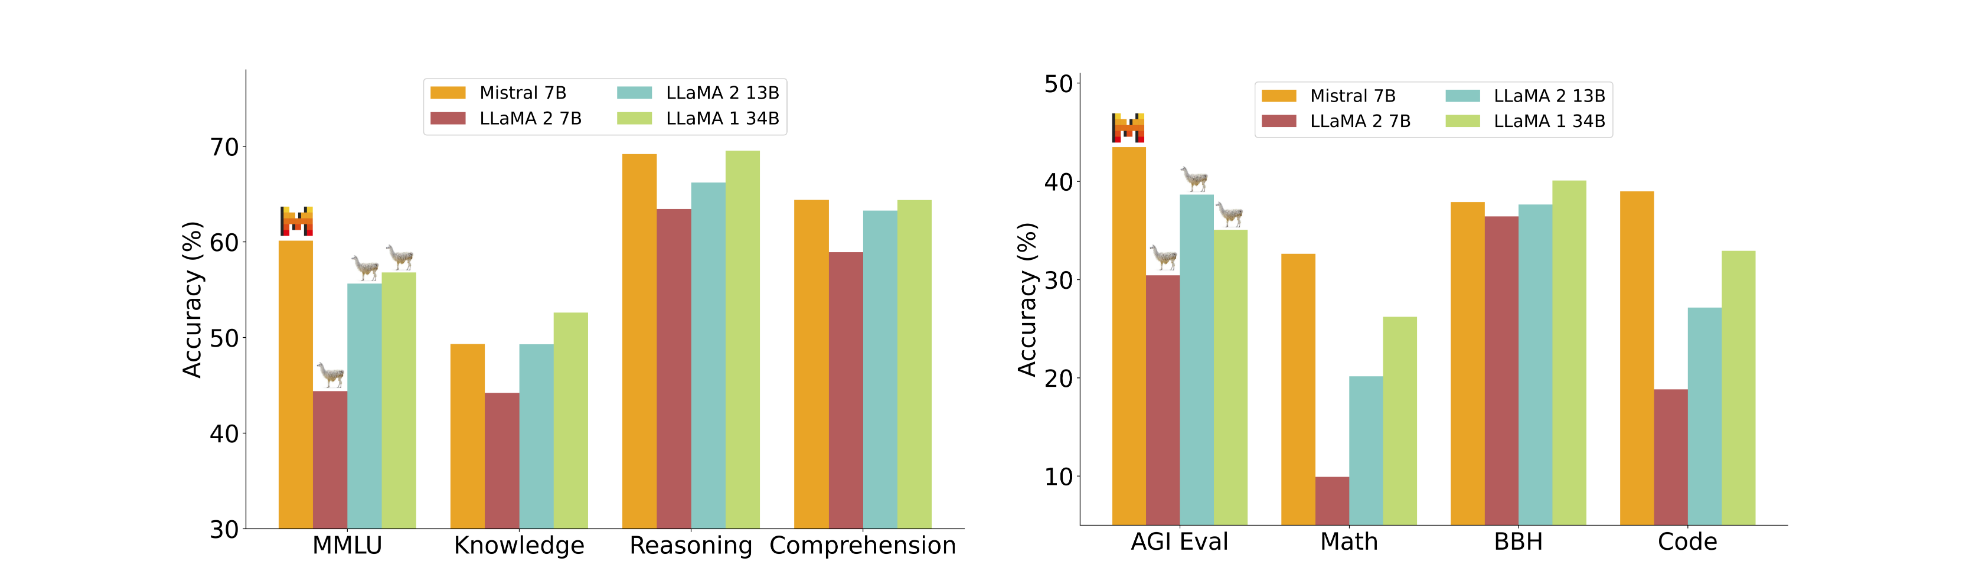
\includegraphics[width=\linewidth]{images/mistral-comparison.png}
    \caption{Confronto fra Mistral e LLama2 su vari task.}
    \label{fig:mistral-vs-lama}
\end{figure}


\section{Metriche di valutazione}
Di seguito vengono riportate le metriche che verranno utilizzate per valutare le performance delle baseline provate. Molti di questi sono diventati uno standard in letteratura per attribuire un punteggio ai modelli di summarization. 

\subsection{Rouge}
Introdotto nel paper \cite{lin-2004-rouge}, l'acronimo \emph{ROUGE} sta per \emph{Recall-Oriented Understudy for Gisting Evaluation} ed è diventato uno degli strumenti più utilizzati per valutare la qualità dei riassunti generati dai modelli, comparandoli anche con quelli creati umanamente.

La ricerca originale propone diverse varianti della metrica ROUGE.

\begin{itemize}
    \item \emph{ROUGE-N}: Misura la sovrapposizione di n-grammi tra il testo generato e il testo di riferimento. La formula seguente
    \begin{equation*}
        \text{ROUGE-N} = \frac{\sum_{S \in \text{Ref}} \sum_{\text{gram}_n \in S} \text{Count}_{Gen}(\text{gram}_n)} {\sum_{S \in \text{Ref}} \sum_{\text{gram}_n \in S} \text{Count}_{Ref}(\text{gram}_n)}
    \end{equation*}
    calcola la somma di tutti gli n-grammi nei riassunti generati e la normalizza dividendola per il numero di n-grammi nei riassunti di riferimento. In questo caso gli n-grammi potranno essere di qualunque dimensione. Se $n=1$ si parla di ROUGE-1, per $n=2$ ROUGE-2 e cosi via.
    \item \emph{ROUGE-L}: Calcola la Lunghezza della Sottosequenza Comune (LCS) tra il testo generato e quello di riferimento.
    \begin{equation*}
        \text{ROUGE-L} = \frac{\sum_{S \in \text{Ref}} LCS(\text{Gen}, S)}{\sum_{S \in \text{Ref}} \vert S \vert}
    \end{equation*}
    La somma delle LCS è normalizzata dividendola per la somma delle lunghezze dei riassunti di riferimento, fornendo una misura della somiglianza fra i testi generati e quelli di riferimento.
    \item \emph{ROUGE-W}: Misura la sovrapposizione di parole basata sulla LCS pesata tra il testo generato e il testo di riferimento.
    \begin{equation*}
        \text{ROUGE-W} = \frac{\sum_{S \in \text{Ref}} WLCS(\text{Gen}, S)}{\sum_{S \in \text{Ref}} \vert S \vert}
    \end{equation*}
    dove $WLCS(\text{Gen}, S)$ non è altro che la lunghezza della sottosequenza comune pesata tra il sistema e un riassunto di riferimento.
\end{itemize}

\subsection{Bleu}
Metrica introdotta nel paper \cite{papineni-etal-2002-bleu} e sta per Bilingual Evaluation Understudy. Anch'essa è ampiamente utilizzata nel contesto delle pubblicazioni relative a task di NLP. In particolare è nata per valutare la qualità delle traduzioni automatiche rispetto a una o più traduzioni di riferimento fornite da umani.
Confronta le corrispondenze n-gram tra il testo tradotto e il testo di riferimento, fornendo un punteggio che indica quanto il testo tradotto sia vicino al testo di riferimento.

Nel contesto di questo progetto si sono utilizzate BLEU-1, BLEU-2, BLEU-3 e BLEU-4 che considerano rispettivamente n-grammi di dimensione 1, 2, 3 e 4.


\subsection{R}

È una metrica utilizzata per avere un valore numerico riassuntivo delle varie ROUGE. Nello specifico rappresenta una media ponderata delle metriche ROUGE, dove la varianza delle metriche ROUGE viene utilizzata come fattore di ponderazione per dare maggiore peso alle metriche con minore varianza. Infatti se una metrica ha una varianza inferiore, significa che è più stabile o consistente attraverso differenti esempi. Dare maggiore importanza alle metriche con minore varianza potrebbe contribuire a ottenere una valutazione più affidabile e meno influenzata da outlier o fluttuazioni casuali nei dati.
Poiché è una metrica non nota in letteratura, di seguito è riportata la formula utilizzata
\begin{equation*}
    R = \frac{\text{mean}(\text{ROUGE-1,ROUGE-2,ROUGE-L})}{1+\text{var}(\text{ROUGE-1,ROUGE-2,ROUGE-L})}
\end{equation*}

dove, dato un set di valori $(x_1, x_2, \dots, x_n)$ media e varianza sono definite come segue
\begin{align*}
    \text{mean}(x_1, x_2, \dots, x_n) &= \frac{1}{n} \sum_{i=1}^n x_i \\
    \text{var}(x_1, x_2, \dots, x_n) &= \frac{1}{n} \sum_{i=1}^n (x_i - \text{mean}(x_1, x_2, \dots, x_n))^2
\end{align*}

\subsection{Bert Score}
Metrica importante per poter ottenere un valore numerico che esprima la vicinanza semantica del riassunto generato e quello di riferimento. 

Come suggerisce il nome, si basa sul modello pre addestrato Bert Score. In particolare, come descritto all'interno del paper \cite{zhang2020bertscore}, BERTScore, in maniera analoga a qualunque altra metrica, produce degli score di similarità numerici fra ogni token generato e ogni token target. 

Tuttavia, piuttosto che valutare dei match esatti, questa similarità è calcolata semanticamente a partire dagli embeddings di Bert. Questo fa si che la metrica sia più simile a una valutazione umana poiché coglie la similarità fra i significati dei due testi.

\subsection{Bart Score}
Metrica proposta nel paper \cite{yuan2021bartscore} per valutare la qualità del testo generato in diverse applicazioni di NLP. La sfida principale in queste applicazioni è valutare se i testi generati siano fluenti, accurati o efficaci. BARTScore affronta questa sfida considerando la valutazione del testo generato come un problema di generazione di testo, modellato utilizzando modelli pre-addestrati di tipo sequence-to-sequence.

Come suggerisce il nome, la metrica utilizza il modello BART per convertire il testo generato in un testo di riferimento o nel testo sorgente, e valuta la qualità del testo generato in base al successo di queste conversioni. In altre parole, se il modello BART riesce a convertire con successo il testo generato nel testo di riferimento o nel testo sorgente, il testo generato viene considerato di alta qualità, e riceverà un punteggio BARTScore più alto.

L'idea generale dietro questo approccio è che i modelli addestrati a convertire il testo generato in un testo di riferimento o nel testo sorgente otterranno punteggi più alti quando il testo generato è di migliore qualità.


\subsection{Mean Cosine Similarity}
La \emph{Similarità Coseno} è una misura di similarità tra due vettori in uno spazio multidimensionale. Può essere usata nel contesto dell'NLP per comparare la similarità tra documenti rappresentati come vettori. 
Come descritto nel Capitolo \ref{cap:tecnologie} è possibile convertire ogni parola in un vettore che preservi la sua semantica. Questo consente di poter fare operazioni vettoriali che si riflettano sulle parole stesse. 

Dati due generici vettori $\mathbf{x}, \mathbf{y}$, la loro similarità si calcola sommando i prodotti sclari dei vettori (sommando i prodotti di coppie di componenti) e dividendo questa quantità per le rispettive norme, cioè
\begin{equation}
    \label{eq:cossim}
    \text{Cosine Similarity} = \frac{\mathbf{x \cdot y}}{\vert \vert \mathbf{x} \vert \vert \vert \vert \mathbf{y} \vert \vert} = 
    \frac{\sum_{i=1}^n x_i y_i}{\sqrt{\sum_{i=1}^n x_i^2} \sqrt{\sum_{i=1}^n y_i^2}}
\end{equation}

Supponiamo ora di avere due rappresentazioni vettoriali di documenti $A, B$ composti da $n$ parole $A_i, B_i$ per $i \in [1, n]$ (anch'essi vettori). La similarità media dei due documenti è data dalla media della similarità coseno \ref{eq:cossim}, per ogni coppia di parole.

\begin{equation*}
    \text{Mean Cosine Similarity} = \frac{1}{n} \sum_{i=1}^n \frac{A_i \cdot B_i}{\vert \vert A_i \vert \vert \vert \vert B_i \vert \vert}
\end{equation*}

I benefici di lavorare sugli angoli come fa, appunto, la \emph{similarità coseno} è quella di non essere influenzati dalla lunghezza dei vettori. Questo risulta molto utile quando occorre calcolare la similarità fra documenti di dimensioni notevolmente diverse. Dunque questa metrica è utile per normalizzare, cioè valutare la proporzione delle occorrenze fra i due testi, piuttosto che la dimensione effettiva.


\subsection{Mean Generation Length}
La \emph{Mean Generation Length} (MGL) è una metrica utilizzata per valutare la lunghezza media delle sequenze o dei testi generati da un modello di generazione del linguaggio naturale. Questa metrica può fornire insight utili sull'abilità di un modello di generare risposte concise o, al contrario, su quanto tende a generare risposte prolisse.

Dato un insieme di $n$ documenti generati, denotati come $\text{prediction}_i$ per $i \in [1,n]$, la MGL è calcolata come segue 

\begin{equation*}
    \text{MGL} = \frac{1}{n} \sum_{i=1}^n \text{len}(\text{prediction}_i)
\end{equation*}

\subsection{Valutazione Umana}
In generale il gold standard per la valutazione di riassunti rimane quella umana. Questa può essere effettuata ponendo particolare attenzione a diverse prospettive. Le più rilevanti per questo progetto sono riportate di seguito
\begin{enumerate}
    \item \emph{Informatività}. Quanto bene il testo generato cattura le idee chiave del testo originale. Questo è particolarmente importante in ottica di summarization in quanto il riassunto deve veicolare tutte le informazioni rilevanti dell'articolo originale. 
    \item \emph{Fattualità}. Verifica se l'ipotesi generata contiene solo affermazioni deducibili dal testo sorgente. Per un riassunto è importante trattare concetti che siano estrapolabili dall'articolo originale, altrimenti perderebbero di significato.
    \item \emph{Copertura Semantica}. Misura quante unità di contenuto semantico dai testi di riferimento sono coperte dal riassunto generato. Come vedremo, poiché gli articoli originali sono molto lunghi, è necessario troncarli prima di fornirli ai modelli, causando un'irreversibile perdita d'informazione. Oltre a questo il riassunto dev'essere notevolmente più breve dell'input, dunque occorre valutare qauli concetti sono stati inclusi e quali no.
\end{enumerate}



































\chapter{Sviluppo}
\label{cap:sviluppo}

Si procede con la descrizione del lavoro svolto sulle fonti per la costruzione del dataset, e lo sviluppo del codice per poter usare le baseline descritte nei capitoli precedenti. 

\section{Creazione del dataset}
Come anticipato,  dopo aver individuato le fonti per l'estrazione dei documenti, è stato sviluppato il codice necessario per poterli raccogliere in un formato semi-strutturato. A questo scopo, si è optato per l'aggregazione dei dati in file \texttt{jsonlines}. I vantaggi di questo formato rispetto ad altri, come ad esempio \texttt{CSV}, includono i seguenti:
\begin{itemize}
    \item \emph{Facilità di elaborazione incrementale}. \texttt{Jsonlines} gestisce un singolo oggetto \texttt{JSON} per riga, rendendo molto più semplice l'elaborazione dei dati in modo incrementale senza dover caricare l'intero set di dati in memoria. Questo lo rende ideale per l'elaborazione di flussi di dati o file di grandi dimensioni.
    \item \emph{Facilità di debug}. A causa di errori nella costruzione del codice o di strutture non consistenti nell'XML, si è reso necessario debuggare i file prodotti. In caso di errori nei dati, è molto più semplice individuare e correggere un errore in una specifica riga di un file \texttt{jsonlines} rispetto a cercarlo all'interno di un grande blocco di \texttt{JSON}. 
    \item \emph{Leggibilità}. Mentre un file \texttt{CSV} definisce il ruolo di ciascuna colonna solo nella prima riga e separa i campi con punti e virgola, spazi, ecc., il formato \texttt{jsonlines} scelto, come illustrato nel Listato \ref{lst:jsonlines}, permette di identificare immediatamente tutti i campi di ogni istanza con una rapida occhiata.
\end{itemize}

\begin{lstlisting}[language=json, 
                   caption=Formato jsonlines articoli.,
                   label=lst:jsonlines]
{
    "doi": "10.1038/s41467-020-16904-3", 
    "pmcid": "PMC7308400",  
    "plain_text": "Single cell RNA-seq is a powerful method to...", 
    "technical_text": "Single-cell RNA sequencing (scRNA-seq) is...", 
    "full_text": "Introduction Tissues are complex milieus comprising...", 
    "journal": "nature communications", 
    "topics": [ "Article" ], 
    "keywords": [ "RNA sequencing", "Computational models", "Software" ]
}
\end{lstlisting}

Poiché non tutti i documenti scaricati presentavano la struttura desiderata (dunque integrassero un summary), si è dovuto fare parsing di questi alla ricerca di tale campo. 
Posto che alcuni documenti possedessero tale riassunto, non tutti utilizzavano lo stesso tag per identificarlo all'interno del \emph{DOM} (Document Object Model). Per questo motivo si è reso necessario un approccio ad'hoc per ogni tipologia di tag identificato a seguito di un'ispezione manuale. 

Di seguito sono riportate le strutture più frequentemente utilizzate per definire tali riassunti 

%% PER PMC010xxxxxx, PMC008xxxxxx
\begin{lstlisting}[language=xml, caption=Struttura XML di un summary., label=lst:xml-pmc10-8]
<sec title="Simple Summary">
  <!-- Contenuto del summary -->
</sec>
\end{lstlisting}

%% PER PMC009xxxxxx
\begin{lstlisting}[language=xml, caption=Struttura XML di un summary., label=lst:xml-pmc9]
<abstract abstract-type="summary">
  <!-- Contenuto del summary -->
</abstract>
\end{lstlisting}

%% PER PMC005xxxxxx
\begin{lstlisting}[language=xml, caption=Struttura XML di un summary., label=lst:xml-pmc5]
<abstract abstract-type="executive-summary">
  <!-- Contenuto del summary -->
</abstract>
\end{lstlisting}

%% PER PMC007xxxxxx
\begin{lstlisting}[language=xml, caption=Struttura XML di un summary., label=lst:xml-pmc7]
<abstract id="Abs">
  <!-- Contenuto del summary -->
</abstract>
\end{lstlisting}


Per fare parsing dei documenti \texttt{XML} si è deciso di utilizzare il modulo \href{https://docs.python.org/3/library/xml.html}{\texttt{xml.etree.ElementTree}} di Python che offre un'API semplice da usare e molto efficiente. 

In particolare è stato utilizzato il seguente script per estrarre una stringa in formato json per ciascun documento il cui summary è nel formato \ref{lst:xml-pmc10-8}.


\begin{python}[caption={Script Python per parsing della sezione `Simple Summary'.}, label={lst:py-pmc10-8}]
import xml.etree.ElementTree as ET

def retrieve_simple_summary(xml_file):
    # Parse the XML file
    tree = ET.parse(xml_file)
    root = tree.getroot()

    # Find the "Simple Summary" section
    summary_section = root.find(".//sec[title='Simple Summary']")
    summary_content = ""
    if summary_section is not None:
        summary_content = ET.tostring(summary_section, encoding='unicode', method='text')
        summary_content = " ".join(summary_content.split()).strip() 
    
    return summary_content
\end{python}

Il codice presentato è molto semplificato e non tiene conto di tutti gli altri campi estratti, per i quali occorrerebbe fare un ragionamento analogo a quello dei summary, in quanto anch'essi non aventi struttura consistente su tutti i documenti.

Si è proceduto analogamente per la tipologia \ref{lst:xml-pmc9} con il seguente codice 

\begin{python}[caption={Python script per estrarre l'abstract di tipo 'summary'.}, label={lst:py-pmc9}]
import xml.etree.ElementTree as ET

def retrieve_summary_abstract(xml_file):
    # Parse the XML file
    tree = ET.parse(xml_file)
    root = tree.getroot()

    # Extract content from the 'summary' type abstract
    summary_abstract = root.find(".//abstract[@abstract-type='summary']")
    summary_content = ""
    if summary_abstract is not None:
        summary_content = ET.tostring(summary_abstract, encoding='unicode', method='text')
        summary_content = " ".join(summary_content.split()).strip() 

    return summary_content
\end{python}

\section{Preprocessamento}

Dopo aver raccolto tutte le istanze di interesse, si è proceduto con l'analisi della qualità del dataset appena creato.

In particolare, si è caricato il file in formato \texttt{jsonlines} all'interno di un \texttt{DataFrame Pandas}. Questa decisione è stata presa basandosi sull'ampio ventaglio di benefici offerti dalla libreria Pandas nella gestione dei dati. Le strutture dati di Pandas, come i DataFrame, sono ottimizzate per l'elaborazione ad alte prestazioni di grandi volumi di dati tabulari.


\subsection{Analisi delle istanze mancanti}
Si è utilizzato il metodo \texttt{df.describe()} per ottenere una panoramica immediata della struttura e distribuzione dei dati. Questo passaggio è cruciale per comprendere la natura del dataset e pianificare eventuali operazioni di preprocessing.

La Tabella \ref{tab:describe_ds} presenta il risultato dell'applicazione di \texttt{df.describe()} al nostro dataset.

\begin{table}[H]
\centering
\begin{tabular}{|l|c|c|c|c|}
\hline
                & Count & Unique & Top                          & Freq  \\ \hline
doi             & 46486 & 44142  &                              & 2345  \\
pmcid           & 46486 & 44143  &                              & 2344  \\
plain\_text     & 46486 & 46470  & We are planning to update... & 2     \\
technical\_text & 46486 & 46478  & Chronic myeloid leukaemia... & 2     \\
full\_text      & 44142 & 44142  & 1. A Commentary on Feed...   & 1     \\
journal         & 46486 & 187    & cancers                      & 8486  \\
topics          & 46486 & 225    & [Article]                    & 21516 \\
keywords        & 46486 & 40577  & []                           & 3601  \\ \hline
\end{tabular}
\caption{Descrizione della struttura e distribuzione del dataset collezionato.}
\label{tab:describe_ds}
\end{table}

Dall'analisi emerge che, delle 46486 istanze raccolte, 44142 sono uniche. Ulteriori indagini sulle 2344 istanze duplicate hanno rivelato che queste, in realtà, non presentano dati nei campi \texttt{doi, pcmid, full\_text}. La Tabella \ref{tab:describe_ds} conferma tale osservazione. Per mantenere la qualità del dataset, si sono quindi eliminate queste istanze con il comando \texttt{df.dropna(subset=[`full\_text'], inplace=True)}.



\section{Analisi Statistica e Visualizzazione dei Dati}
Una volta corrette le anomalie nei dati, l'attenzione si è spostata sull'analisi statistica del dataset, con un occhio di riguardo verso la rilevazione di \emph{outliers}, ovvero quelle istanze che si discostano significativamente dalla norma.

\subsection{Distribuzione per Rivista Scientifica}
Per meglio comprendere la composizione del dataset e facilitarne il caricamento su HuggingFace, suddiviso per rivista, si è stimata la distribuzione delle istanze per ciascuna pubblicazione. Utilizzando il codice Python riportato di seguito, sono state filtrate e visualizzate solo le riviste che rappresentano più dell'1\% del totale, assegnando le altre alla categoria ``Others''.

\begin{python}[caption={Codice Python per graficare la distribuzione delle riviste.}, label={lst:py-distrib-riv}]
journal_counts = articles["journal"].value_counts()

filtered_journal_counts = journal_counts[journal_counts / journal_counts.sum() > 0.01]

mask = articles["journal"].isin(filtered_journal_counts.index)

articles.loc[~mask, "journal"] = "Others"

filtered_article_counts = articles["journal"].value_counts()

plt.figure(figsize=(10, 10))
filtered_article_counts.plot.pie(autopct='%1.1f%%')
plt.axis('equal')
plt.show()
\end{python}

Questo approccio ha prodotto il grafico a torta in Figura \ref{fig:journal-inst-perc}, che illustra la percentuale di istanze per ciascuna rivista. La decisione di escludere le riviste con meno dell'1\% delle istanze è stata presa per evitare di avere split del dataset con un numero insufficiente di dati, garantendo così una rappresentazione equilibrata.


\subsection{Analisi della Frequenza dei Dati}
Per valutare la dimensione degli attributi pertinenti agli esperimenti, sono stati realizzati degli istogrammi che evidenziassero le distribuzioni di frequenza di interesse.

\subsubsection{Frequenza del numero di caratteri}
L'analisi è iniziata esaminando la lunghezza dei testi, misurata dal numero di caratteri per le sezioni \texttt{plain\_text}, \texttt{technical\_text} e \texttt{full\_text}. Si è prodotto un grafico congiunto per i primi due e un grafico separato per il testo completo, a causa delle loro diverse dimensioni.

Il codice utilizzato per visualizzare la distribuzione della lunghezza degli articoli è il seguente:

\begin{python}[caption={Python script per visualizzare le distribuzioni di frequenza delle lunghezze degli articoli.}, label={lst:py-plt-hist}]
import matplotlib.pyplot as plt

plain_text_lengths = articles["plain_text"].str.len()
technical_text_lengths = articles["technical_text"].str.len()

plt.figure(figsize=(10, 5))

plt.hist(plain_text_lengths, bins=100, alpha=0.5, label="Plain Text")

plt.hist(technical_text_lengths, bins=100, alpha=0.5, label="Technical Text")

plt.title("Summary and Technical Text Length Distribution")
plt.xlabel("Length")
plt.ylabel("Frequency")
plt.legend()

plt.xlim(0, 20000) 
plt.xticks(range(0, 20001, 4000)) 

plt.show()
\end{python}
Gli istogrammi risultanti mostrano che il \texttt{technical\_text} presenta una notevole varianza, con molti valori anomali che vanno da 4000 a 20000 caratteri, mentre il \texttt{plain\_text} appare più omogeneo. Il \texttt{full\_text}, invece, evidenzia alcuni valori anomali con oltre 10000 caratteri.
Le distribuzioni ottenute sono mostrate in Figure \ref{fig:hist_tech_plain} per technical e plain, e \ref{fig:hist_full} per full.
\begin{figure}
    \centering
    \begin{subfigure}[b]{0.89\textwidth}
        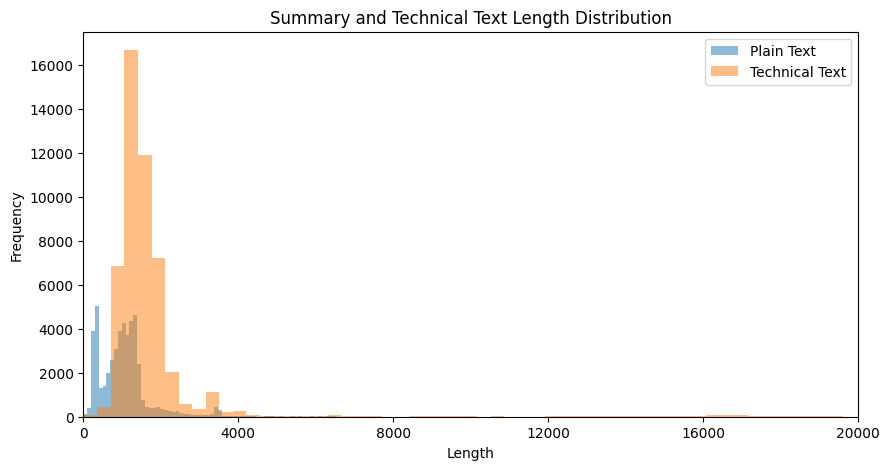
\includegraphics[width=\textwidth]{images/sum_tech_length_distrib.png}
        \caption{Frequenza numero di caratteri per plain e technical text.}
        \label{fig:hist_tech_plain}
    \end{subfigure}
\quad
    \begin{subfigure}[b]{0.85\textwidth}
        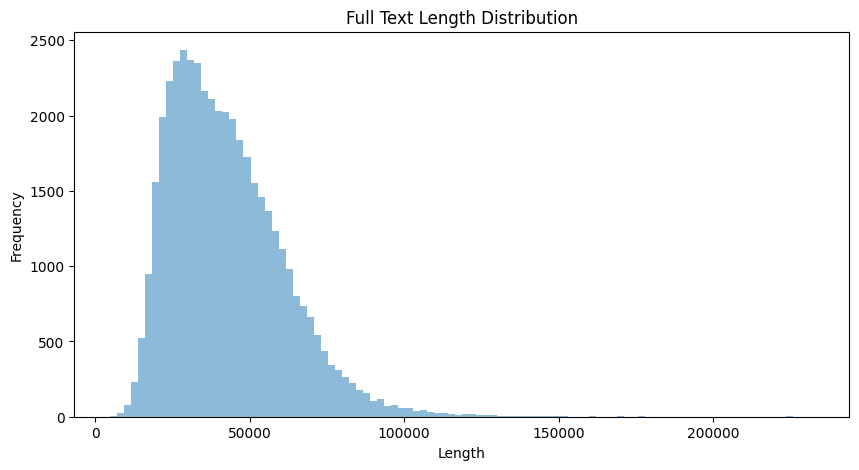
\includegraphics[width=\textwidth]{images/full_length_distrib.png}
        \caption{Frequenza numero di caratteri per full text.}
        \label{fig:hist_full}
    \end{subfigure}
    \caption{Istogrammi per il numero di caratteri.}
\end{figure}


\subsubsection{Frequenza del numero di parole}
La tokenizzazione, eseguita con \texttt{nltk.tokenize}, ha permesso di calcolare il conteggio medio delle parole per sezione, con risultati che corrispondono alle aspettative: il \texttt{plain\_text} è il più conciso, seguito da \texttt{technical\_text} e poi da \texttt{full\_text}, il più esteso. La media del conteggio delle parole è presentata nella Tabella \ref{tab:avg_word_count}.

\begin{table}
\centering
\begin{tabular}{|l|c|}
\hline
Sezione         & Avg Word Count \\ \hline
Plain Text      & 144.87 \\ \hline
Technical Text  & 238.61 \\ \hline
Full Text       & 7615.55 \\ \hline
\end{tabular}
\caption{Numero medio di parole per ogni sezione di un articolo.}
\label{tab:avg_word_count}
\end{table}

Il codice impiegato è il seguente

\begin{python}[caption={Tokenizzazione delle istanze e calcolo dei valori medi.}, label={lst:py-tok-word-count}]
from nltk.tokenize import word_tokenize
nltk.download('punkt')
articles['plain_word_count'] = articles['plain_text'].apply(lambda text: len(word_tokenize(text)))
articles['technical_word_count'] = articles['technical_text'].apply(lambda text: len(word_tokenize(text)))
articles['full_word_count'] = articles['full_text'].apply(lambda text: len(word_tokenize(text)))
print(articles['plain_word_count'].mean(),
       articles['technical_word_count'].mean(),
       articles['full_word_count'].mean())
\end{python}

Per una visualizzazione dettagliata, si sono poi generati istogrammi per il conteggio delle parole utilizzando un codice simile a quello precedentemente descritto. Questi istogrammi hanno confermato i problemi individuati con il \texttt{technical\_text}, rivelando un numero significativo di outliers con un conteggio parole che oscilla tra 1000 e 3200, a dispetto di una media di circa 238 parole. Analogamente, l'analisi del \texttt{full\_text} ha svelato alcune istanze sotto i 1000 caratteri e altre che eccedevano i 20000, sebbene in minor numero.

\begin{python}[caption={Script per graficare le distribuzioni di frequenza del numero di parole.}, label={lst:py-freq-par}]
import matplotlib.pyplot as plt

plt.figure(figsize=(10, 5))

plt.hist(articles["plain_text_word_count"], bins=100, alpha=0.5, label="Plain Text Words")

plt.hist(articles["technical_text_word_count"], bins=100, alpha=0.5, label="Technical Text Words")

plt.title("Summary and Technical Text Word Count Distribution")
plt.xlabel("Words Count")
plt.ylabel("Frequency")
plt.legend()

plt.xlim(0, 4000)
plt.xticks(range(0, 4001, 400))

plt.show()
\end{python}

Come nel caso precedente, si è scelto di presentare un unico script per prevenire ridondanze. Dai grafici risultanti, illustrati nelle Figure \ref{fig:hist_tech_plain_word} per il testo semplice e tecnico e nella Figura \ref{fig:hist_full_word} per il testo completo, emergono le distribuzioni di interesse.

\begin{figure}
    \centering
    \begin{subfigure}[b]{0.89\textwidth}
        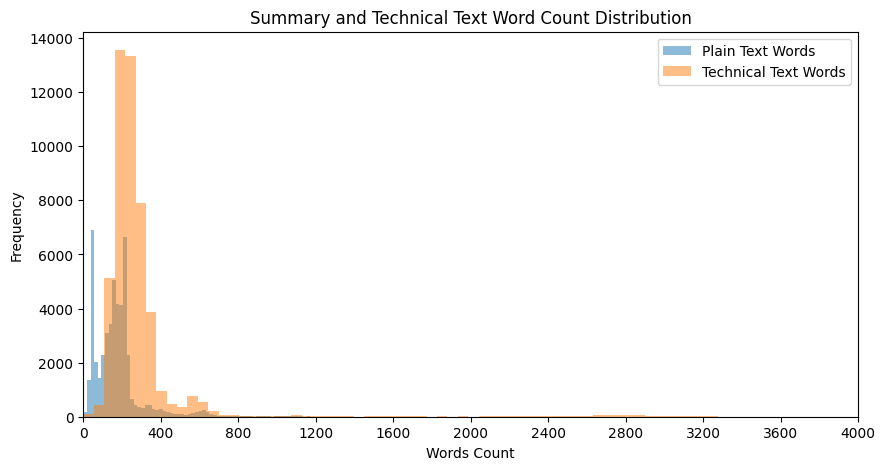
\includegraphics[width=\textwidth]{images/sum_tech_wc_distrib.png}
        \caption{Frequenza numero di parole per plain e technical text.}
        \label{fig:hist_tech_plain_word}
    \end{subfigure}
\quad
    \begin{subfigure}[b]{0.85\textwidth}
        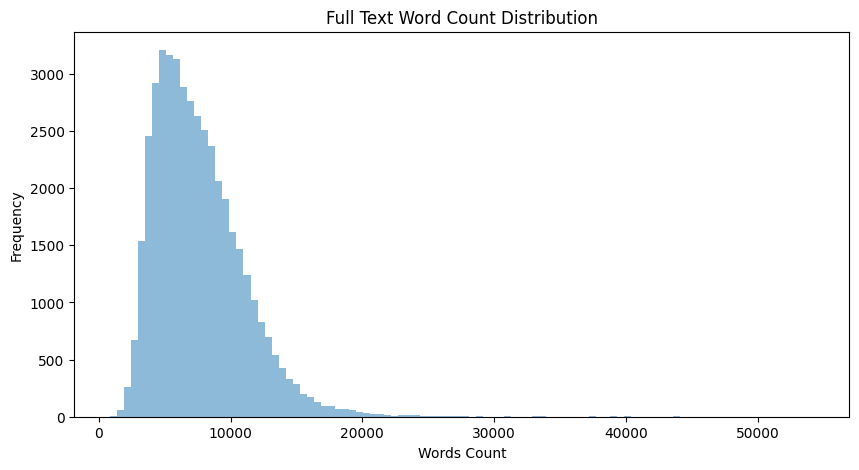
\includegraphics[width=\textwidth]{images/full_text_wc_distrib.png}
        \caption{Frequenza numero di parole per full text.}
        \label{fig:hist_full_word}
    \end{subfigure}
    \caption{Istogrammi per il numero di parole.}
\end{figure}


\subsubsection{Coverage Density e Compression degli articoli}
Fino a questo momento ci si è concentrati su caratteristiche inerenti alle varie sezioni prese singolarmente. Un altro fattore molto importante da valutare è anche la relazione che intercorre fra le sezioni di \texttt{technical\_text}, \texttt{plain\_text} e \texttt{full\_text}. In particolare si è deciso di considerare
\begin{itemize}
    \item \textbf{Coverage}. È una misura che riflette la proporzione del testo target (in questo caso \texttt{technical\_text} o \texttt{plain\_text}) che è stata ritrovata nel testo source (\texttt{full\_text}). Essa è concepita per valutare quanto contenuto di un dato testo è coperto o incluso in un altro. Si calcola con 
    \begin{equation*}
        \text{Coverage} = \frac{\sum (\text{Match Length})}{\text{Total Length of Target Text}}
    \end{equation*}
    dove al numeratore vengono sommate tutte le lunghezze delle sequenze di parole uguali in testo di riferimento e target e al denominatore la lunghezza totale del testo target.
    \item \textbf{Density}. Rappresenta quanto intensamente le corrispondenze tra il testo target e il testo source sono concentrate. Se il testo target ha molte corrispondenze lunghe e ininterrotte nel testo source, la density sarà alta. Formalmente vale
    \begin{equation*}
        \text{Density} = \frac{\sum (\text{Match Length})^2}{\text{Total Length of Target Text}}
    \end{equation*}
    Elevare al quadrato la lunghezza di ogni corrispondenza dà più peso a corrispondenze più lunghe e ininterrotte rispetto a molte corrispondenze brevi.
    \item \textbf{Compression}. Rappresenta il rapporto tra la lunghezza del testo source e la lunghezza del testo target. Questa metrica è utile per comprendere quanto il testo target sia più conciso rispetto al testo source. La formula è questa
    \begin{equation*}
        \text{Compression} = \frac{\text{Total Length of Source Text}}{\text{Total Length of Target Text}}
    \end{equation*}
    Valori di compressione alti potrebbero indicare che il testo sorgente sia notevolmente più lungo del target, che dunque potrebbe risultare poco rappresentativo. Viceversa, valori inferiori a 1 vorrebbero dire che il target sia inspiegabilmente più lungo del riferimento.
\end{itemize}

Nella tabella \ref{tab:cov_dens_compr} è riportato il valore medio per ogni metrica. Si nota che coverage e density risulta di fatto equivalente fra technical e plain, probabilmente dovuto al fatto che in entambi vi è lo stesso quantitativo di sequenze di parole identiche. Da notare, invece, che la compression è oltre il doppio per plain rispetto a technical, questo fa capire come tipicamente il technical text sia di dimensione molto più elevata rispetto al plain.


\begin{table}
\centering
\begin{tabular}{|c|c|c|}
\hline
            & Plain Text & Technical Text \\ \hline
Coverage    & 0.9        & 0.93           \\ \hline
Density     & 3.07       & 3.67           \\ \hline
Compression & 78.05      & 35.04          \\ \hline
\end{tabular}
\caption{Coverage Density e Compression degli articoli.}
\label{tab:cov_dens_compr}
\end{table}


Oltre a questo, sono state graficate tramite istogrammi le distribuzioni di ciascuna di queste metriche. Di rilevanza è la compression per cui si sono notate alcune istanze fuori range mostrate in Figura \ref{fig:hist_compression_plain} e \ref{fig:hist_compression_tech}.




\subsection{Rimozione degli outliers}
Come anticipato, dai grafici in Figura \ref{fig:hist_tech_plain_word}, \ref{fig:hist_full_word}, emergono degli \emph{outliers} con numero di parole anomale rispetto alla media, sia per \texttt{technical\_text} che per \texttt{full\_text}. 

Affinché il dataset sia coerente ed omogeneo, si è deciso di scartare questi valori anomali optando per lasciare solo quelli il cui numero di parole non superi le 800 per summary e technical (in quanto le loro frequenze sono quasi equivalenti). Per quanto riguarda full si sono tenute le istanze con parole comprese fra 1000 e 20000.

Le Figure \ref{fig:hist_tech_plain_word_outliers} e \ref{fig:hist_full_word_outliers} mostrano graficamente i valori che sono stati scartati.

\begin{figure}
    \centering
    \begin{subfigure}[b]{0.89\textwidth}
        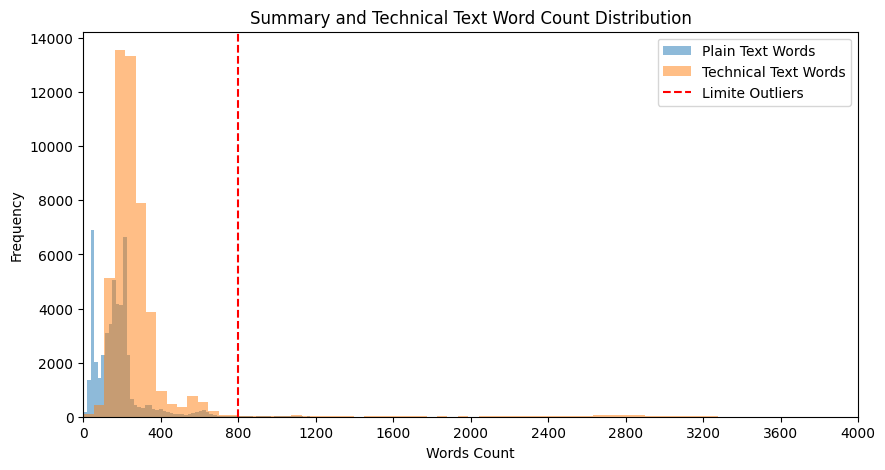
\includegraphics[width=\textwidth]{images/hist_wc_outliers.png}
        \caption{Outliers per plain e technical.}
        \label{fig:hist_tech_plain_word_outliers}
    \end{subfigure}
\quad
    \begin{subfigure}[b]{0.85\textwidth}
        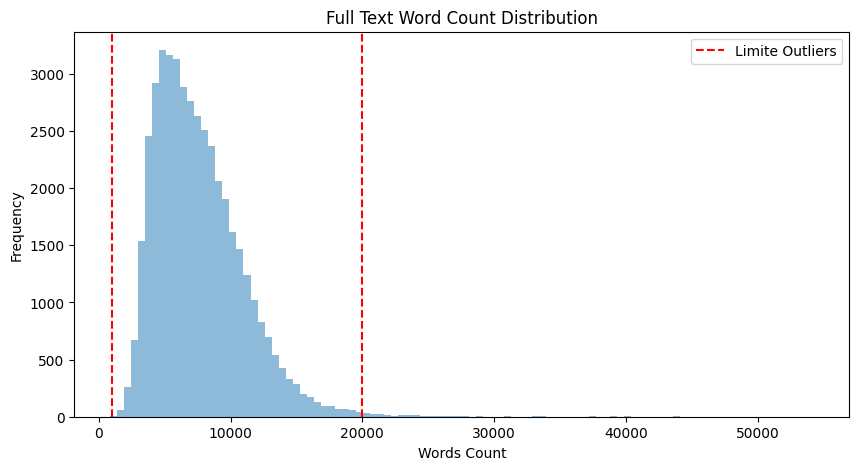
\includegraphics[width=\textwidth]{images/hist_wc_outliers_full.png}
        \caption{Outliers per full text.}
        \label{fig:hist_full_word_outliers}
    \end{subfigure}
    \caption{Visualizzazione degli outliers.}
\end{figure}

Per farlo si è impiegato il seguente codice che consente, grazie alla potenza di \texttt{Pandas}, di scartare tutte le istanze indesiderate in una sola volta.

\begin{python}[caption={Script per rimozione outliers per numero di parole.}, label={lst:py-rimuovi-outliers}]
articles = articles[(articles["technical_text_word_count"] <= 800) & 
                     (articles["plain_text_word_count"] <= 800) &
                     (articles["full_text"] >= 1000) &
                     (articles["full_text"] <= 20000)]
\end{python}


Questo ha portato a delle distribuzioni più significative che, se plottate, mostrano in maniera più chiara con che frequenza compaino gli articoli aventi un certo numero di parole. Queste sono visibili in Figura \ref{fig:updated_hist_wc} per plain e tecnhnical. Per \texttt{full\_text} non è mostrata poiché molto simile a \ref{fig:hist_full_word}.

\begin{figure}
    \centering
    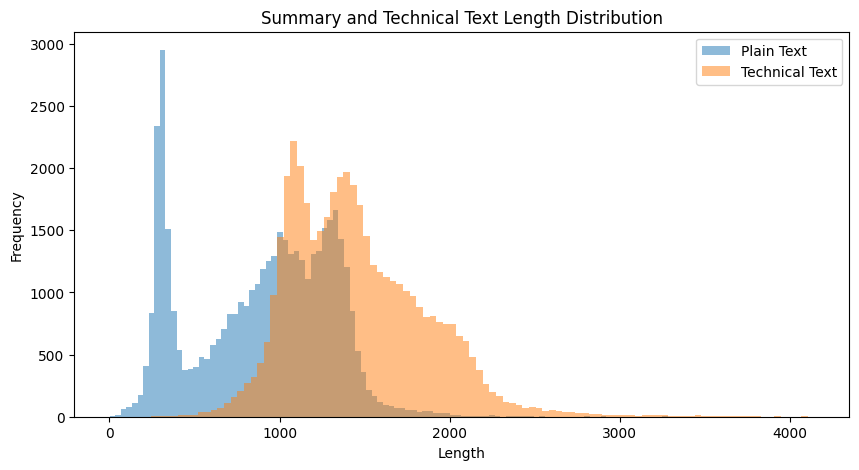
\includegraphics[width=0.75\linewidth]{images/updated_hist_wc.png}
    \caption{Istogramma numero di parole per plain e technical texts post pulizia outliers.}
    \label{fig:updated_hist_wc}
\end{figure}


Fatto ciò si sono rimosse le istanze che avessero compression oltre un limite soglia definito su 400 per plain e 135 per technical. Graficamente si vede in Figura \ref{fig:hist_compression_plain}, \ref{fig:hist_compression_tech}.

\begin{figure}
    \centering
    \begin{subfigure}[b]{0.85\textwidth}
        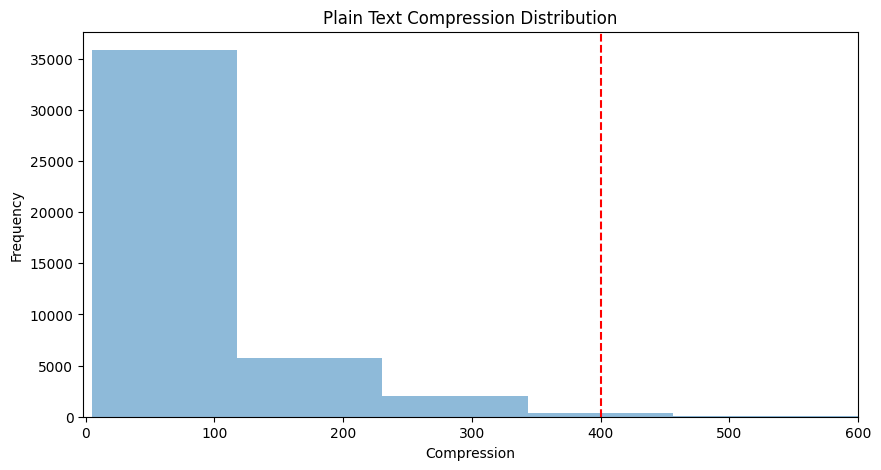
\includegraphics[width=\linewidth]{images/hist_compression_plain.png}
        \caption{Outliers Compression Plain Text.}
        \label{fig:hist_compression_plain}
    \end{subfigure}
\quad
    \begin{subfigure}[b]{0.85\textwidth}
        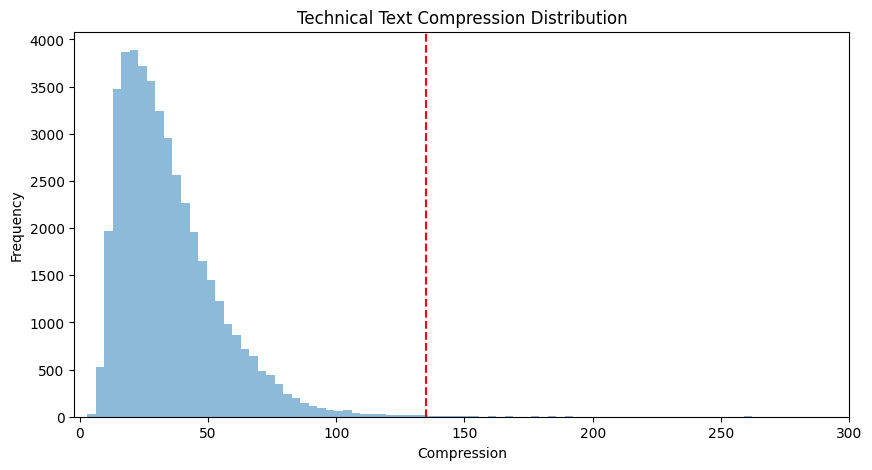
\includegraphics[width=\linewidth]{images/hist_compression_technical.png}
        \caption{Outliers Compression Full Text.}
        \label{fig:hist_compression_tech}
    \end{subfigure}
    \caption{Visualizzazione degli Outliers per Compression.}
\end{figure}

\subsection{Caricamento del dataset su HuggingFace}
Pulito il dataset dalle istanze non desiderate, si è caricato il dataset su HuggingFace. Per fare questo si è usato come riferimento il dataset \href{https://huggingface.co/datasets/big_patent}{BigPatent}. Affinchè il dataset venga caricato correttamente è necessario disporre le istanze in file compressi (\texttt{.zip}) aventi come nome lo split di appartenenza (i.e. train, test, validation). All'interno di questi zip è stato necessario dividere le istanze in directory, una per ogni rivista. I file \texttt{.zip} devono poi essere inseriti nel percorso \texttt{data/version/}. Per fare questo si è impiegato il seguente codice che divide automaticamente i dati in train validation e test, in un rapporto 80, 10, 10 e li dispone nelle cartelle corrette.
Per poter identificare quelle riviste che andassero sotto la categoria ``Others'' si è definito un dizionario con i nomi delle riviste mostrate in Figura \ref{fig:journal-inst-perc} (e le rispettive abbreviazioni). Tutte le istanze la cui rivista non rientrasse all'interno di questo dizionario venivano inserite appunto nella categoria ``Others''.
Il codice è il seguente 

\begin{python}
_VERSION = "1.0.0"

_JOURNALS = { ... } 

def split_and_save(examples, journal_name):
    train, validate, test = np.split(examples.sample(frac=1, random_state=42), 
                                     [int(.8*len(examples)), int(.9*len(examples))])
    for subset, kind in zip([train, validate, test], ['train', 'validation', 'test']):
        subdir = f"sci_lay/data/{_VERSION}/{kind}/{_JOURNALS.get(journal_name, 'OTHER')}"
        save_examples(subset.to_dict(orient="records"), subdir)
    print(f"Journal '{journal_name}' correctly split into train/validation/test.")

def save_examples(examples, output_dir):
    os.makedirs(output_dir, exist_ok=True)
    file_path = os.path.join(output_dir, f"{os.path.basename(output_dir)}.jsonl")
    with open(file_path, "a") as file:
        for example in examples:
            file.write(json.dumps(example) + "\n")

others = []
for journal, examples in dataset.groupby("journal"):
    if journal.lower() in _JOURNALS:
        split_and_save(examples, journal.lower())
    else:
        others.append(examples)

if others:
    other_examples = pd.concat(others, ignore_index=True)
    split_and_save(other_examples, 'OTHER')

\end{python}
















%% CAPITOLO 5
\chapter{Il codice prodotto}
\label{cap:codice}

Si elencano i passaggi svolti per raggiungere i risultati descritti in precedenza.

\hypertarget{preprocessamento-dati}{%
\section{Preprocessamento dati}\label{preprocessamento-dati}}

    \hypertarget{caricamento-dati-e-librerie}{%
\subsection{Caricamento dati e
librerie}\label{caricamento-dati-e-librerie}}

    \begin{Verbatim}[commandchars=\\\{\}]
{\color{incolor}In [{\color{incolor}1}]:} \PY{k+kn}{import} \PY{n+nn}{numpy} \PY{k}{as} \PY{n+nn}{np}
        \PY{k+kn}{import} \PY{n+nn}{pandas} \PY{k}{as} \PY{n+nn}{pd}
        \PY{k+kn}{import} \PY{n+nn}{scipy} \PY{k}{as} \PY{n+nn}{sc}
        \PY{k+kn}{from} \PY{n+nn}{tqdm} \PY{k}{import} \PY{n}{tqdm\PYZus{}notebook}
        \PY{k+kn}{from} \PY{n+nn}{time} \PY{k}{import} \PY{n}{sleep}
\end{Verbatim}


    \begin{Verbatim}[commandchars=\\\{\}]
{\color{incolor}In [{\color{incolor}2}]:} \PY{c+c1}{\PYZsh{} GLOBAL SETTINGS}
        \PY{n}{CHECK\PYZus{}ALL\PYZus{}CODES\PYZus{}IN\PYZus{}COUPLES} \PY{o}{=} \PY{k+kc}{False}
\end{Verbatim}


    \begin{Verbatim}[commandchars=\\\{\}]
{\color{incolor}In [{\color{incolor} }]:} \PY{n}{all\PYZus{}data} \PY{o}{=} \PY{n}{pd}\PY{o}{.}\PY{n}{read\PYZus{}csv}\PY{p}{(}
            \PY{l+s+s2}{\PYZdq{}}\PY{l+s+s2}{Totale.csv}\PY{l+s+s2}{\PYZdq{}}\PY{p}{,}
            \PY{n}{sep}\PY{o}{=}\PY{l+s+s2}{\PYZdq{}}\PY{l+s+s2}{;}\PY{l+s+s2}{\PYZdq{}}\PY{p}{,}
            \PY{n}{usecols}\PY{o}{=}\PY{p}{[}\PY{l+s+s2}{\PYZdq{}}\PY{l+s+s2}{DESCRIZIONE}\PY{l+s+s2}{\PYZdq{}}\PY{p}{,} \PY{l+s+s2}{\PYZdq{}}\PY{l+s+s2}{CODICE}\PY{l+s+s2}{\PYZdq{}}\PY{p}{,} \PY{l+s+s2}{\PYZdq{}}\PY{l+s+s2}{AZIENDA}\PY{l+s+s2}{\PYZdq{}}\PY{p}{]}\PY{p}{)}
        \PY{n}{accop} \PY{o}{=} \PY{n}{pd}\PY{o}{.}\PY{n}{read\PYZus{}csv}\PY{p}{(}
            \PY{l+s+s2}{\PYZdq{}}\PY{l+s+s2}{Appaiamenti al 07\PYZus{}09\PYZus{}2018.csv}\PY{l+s+s2}{\PYZdq{}}\PY{p}{,}
            \PY{n}{sep}\PY{o}{=}\PY{l+s+s2}{\PYZdq{}}\PY{l+s+s2}{;}\PY{l+s+s2}{\PYZdq{}}\PY{p}{,}
            \PY{n}{usecols}\PY{o}{=}\PY{p}{[}\PY{l+s+s2}{\PYZdq{}}\PY{l+s+s2}{DESCRIZIONE}\PY{l+s+s2}{\PYZdq{}}\PY{p}{,} \PY{l+s+s2}{\PYZdq{}}\PY{l+s+s2}{CODICE}\PY{l+s+s2}{\PYZdq{}}\PY{p}{,} \PY{l+s+s2}{\PYZdq{}}\PY{l+s+s2}{AZIENDA}\PY{l+s+s2}{\PYZdq{}}\PY{p}{,}
                \PY{l+s+s2}{\PYZdq{}}\PY{l+s+s2}{codice\PYZus{}regionale}\PY{l+s+s2}{\PYZdq{}}\PY{p}{]}\PY{p}{)}
\end{Verbatim}


    \hypertarget{unione-dei-dataframe}{%
\subsection{Unione dei dataframe}\label{unione-dei-dataframe}}

    \begin{Verbatim}[commandchars=\\\{\}]
{\color{incolor}In [{\color{incolor}4}]:} \PY{n}{all\PYZus{}data} \PY{o}{=} \PY{n}{pd}\PY{o}{.}\PY{n}{merge}\PY{p}{(}
            \PY{n}{all\PYZus{}data}\PY{p}{,}
            \PY{n}{accop}\PY{p}{,}
            \PY{n}{how}\PY{o}{=}\PY{l+s+s1}{\PYZsq{}}\PY{l+s+s1}{outer}\PY{l+s+s1}{\PYZsq{}}\PY{p}{,}
            \PY{n}{on}\PY{o}{=}\PY{p}{[}\PY{l+s+s2}{\PYZdq{}}\PY{l+s+s2}{AZIENDA}\PY{l+s+s2}{\PYZdq{}}\PY{p}{,} \PY{l+s+s2}{\PYZdq{}}\PY{l+s+s2}{CODICE}\PY{l+s+s2}{\PYZdq{}}\PY{p}{,} \PY{l+s+s2}{\PYZdq{}}\PY{l+s+s2}{DESCRIZIONE}\PY{l+s+s2}{\PYZdq{}}\PY{p}{]}\PY{p}{)}
        \PY{k}{assert} \PY{n}{all\PYZus{}data}\PY{o}{.}\PY{n}{codice\PYZus{}regionale}\PY{o}{.}\PY{n}{count}\PY{p}{(}
        \PY{p}{)} \PY{o}{==} \PY{n}{accop}\PY{o}{.}\PY{n}{shape}\PY{p}{[}\PY{l+m+mi}{0}\PY{p}{]}
\end{Verbatim}




%% CONCLUSIONI

\chapter*{Conclusioni e sviluppi futuri}
\addcontentsline{toc}{chapter}{Conclusioni e sviluppi futuri}
\markboth{CONCLUSIONI}{CONCLUSIONI}

Il problema iniziale richiedeva l'utilizzo di un algoritmo abbastanza intelligente da poter accoppiare brevi testi etichettati come \emph{simili}.

Dopo aver utilizzato e testato entrambe le tecnologie disponibili nel campo del deep learning (applicato al natural language processing) si è giunti alla conclusione che Doc2Vec, l'algoritmo non supervisionato, fa molta fatica quando i testi non sono semanticamente corretti e logici, e quanto sono presenti molte abbreviazioni.

Al contrario, 

%% RINGRAZIAMENTI
\chapter*{Ringraziamenti}
\addcontentsline{toc}{chapter}{Ringraziamenti}
\markboth{RINGRAZIAMENTI}{RINGRAZIAMENTI}

Il primo ringraziamento va al relatore di questo lavoro, il Prof. Gianluca Moro, che ha reso possibile tutto ciò e ha acceso il mio personale interesse nei confronti di questa splendida disciplina.

Grazie alla mia ...
	
\backmatter	
\addcontentsline{toc}{chapter}{Bibliografia}
\bibliographystyle{unsrt}
% i riferimenti bibliografici, che devono essere almeno 20 per una tesi triennale ed almeno 30 per una della magistrale, si scaricano da qui https://dblp.uni-trier.de/search/
% e si aggiungono al file bibliografia.bib, dopodichè si citano opportuanamente nel testo della tesi con \cite{label}  dove label è il primo elemento di ogni rif. bibliografico subito dopo la parentesi graffa aperta, e.g. DBLP:books/daglib/0087929 (vedi file .bib sopra menzionato)
\bibliography{bibliografia}


\end{document}
